\section{Change of prior}
For any choice of prior, there will be some parameterization in which the prior density is constant (that is, uniform or flat). The difficult question to answer is: in which parameterization ought the prior density be constant? In the pMSSM paper, the ur-prior (coined by Glen Cowan from the German prefix {\it ur} meaning original or primitive), is taken to be uniform in a physically motivated parameterization. However, \emph{a priori} it is not clear that this
is the parameterization in which the prior should be flat.  
Foregoing a discussion of how best to choose a parametrization,  it is examined how the results are affected when the choice of ur-prior is changed.

Figures \ref{fig:mg_prepost}-\ref{fig:mApole} show the prior and posterior density projections onto a suite of parameters presented in the paper \cite{pMSSMpaper}, given the choice of a flat prior (red) and a prior proportional to the product of the log of each parameter (blue), referred to here as the log prior. The main conclusions of the paper stand with respect to this change, namely that
\begin{itemize}
\item pMSSM points with gluino masses below 500 GeV are excluded, but a small number points with 550 GeV gluinos survive (Fig. \ref{fig:mg});
\item the probability density of the light top squark mass is not significantly shifted by the CMS analyses (Fig. \ref{fig:mt1});
\item no LSP mass or $\tilde{\chi}^{\pm}$ mass can be excluded (Fig. \ref{fig:mz1}), and
\item the most probable value (MPV) of the signal cross section has been pushed down by a factor of 10 (Fig. \ref{fig:xsect}).
\end{itemize}
The posterior MPVs for most parameters agree within 5\% between the flat and log priors. The most significant difference is in the impact on the LSP mass, where the log prior prefers slightly larger values of the LSP mass (Fig. \ref{fig:mz1}). This is because the LSP in general exhibits a high density in the low mass region, and this region is suppressed due to the log Jacobian.  The result is that the bulk of the prior and posterior is shifted down.


\begin{figure}[h]
\centering
\subfloat[]{
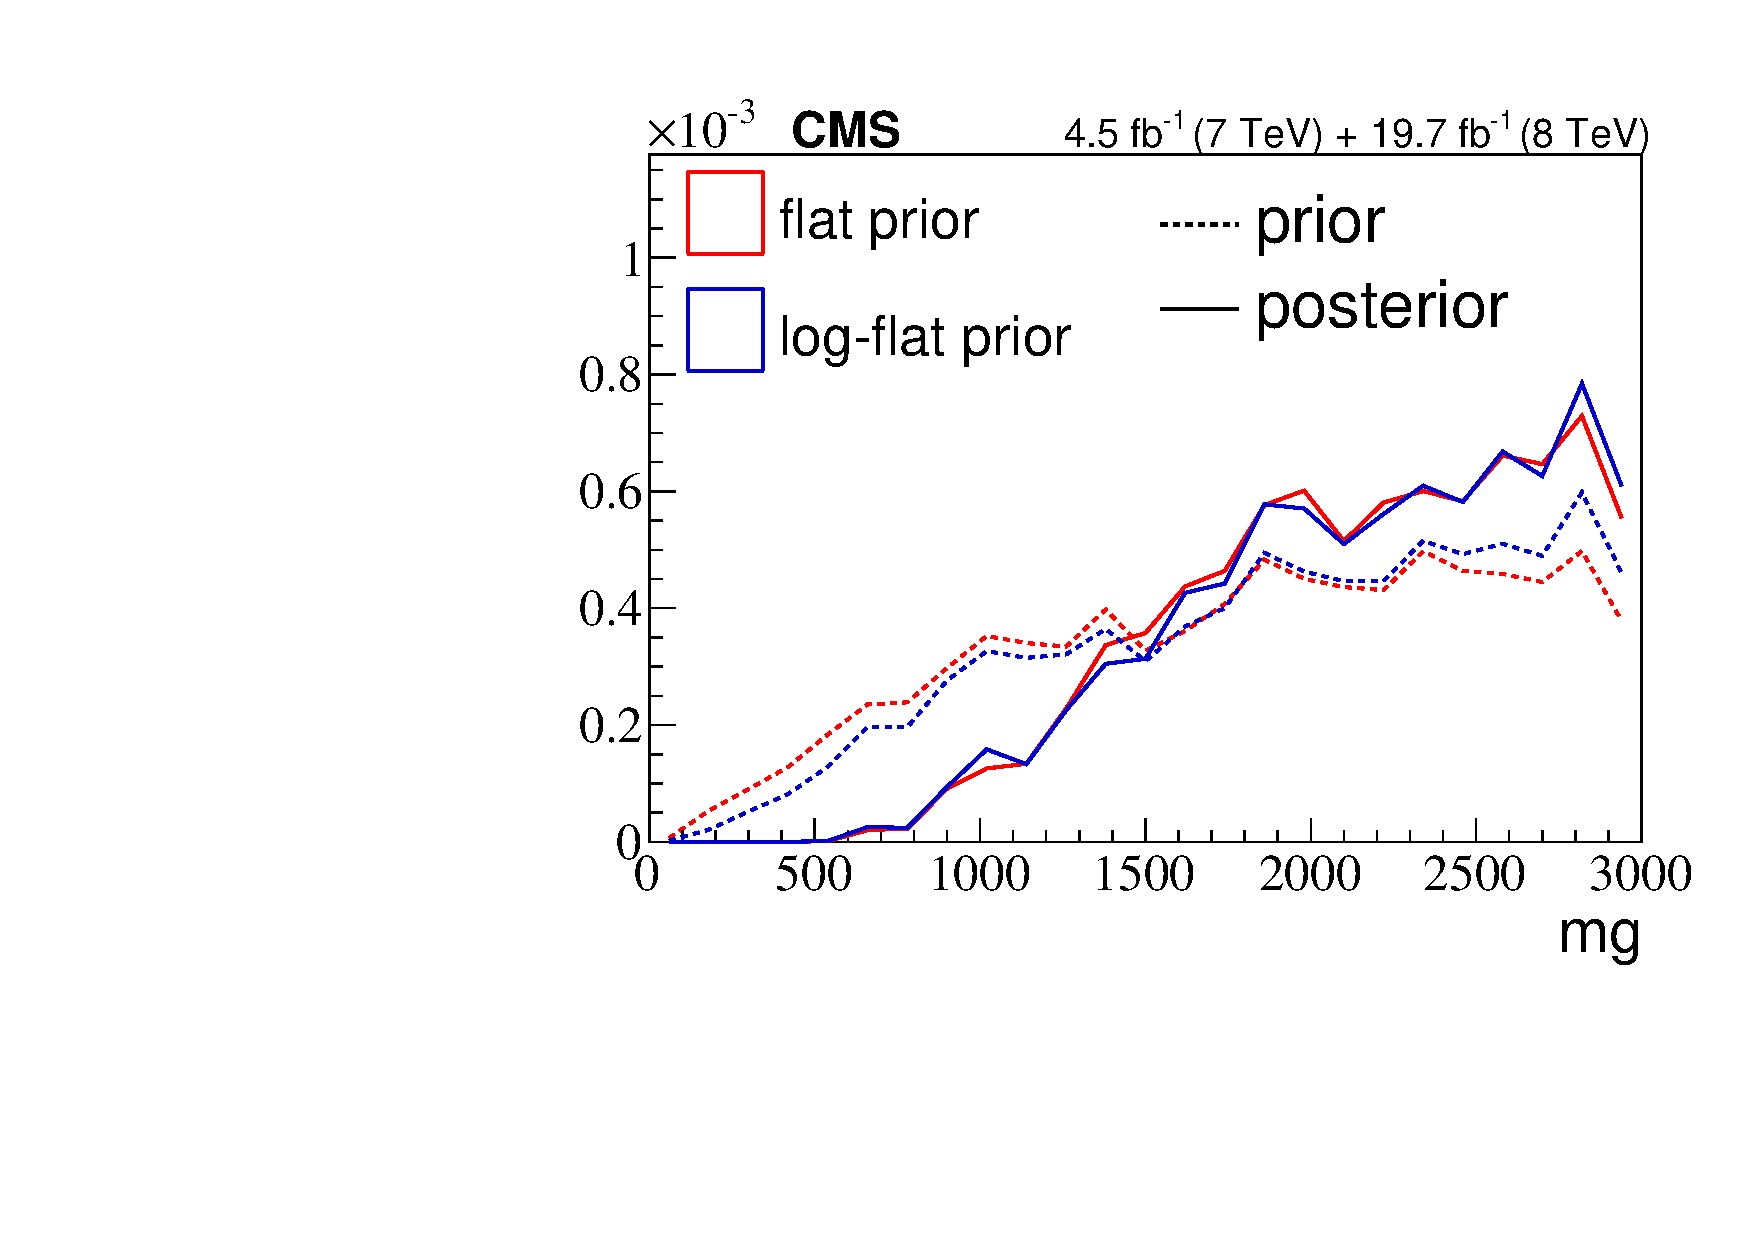
\includegraphics[width=0.5\linewidth]{figures/pMSSMpaper/Prior/mgprepost.pdf}
}
\subfloat[]{
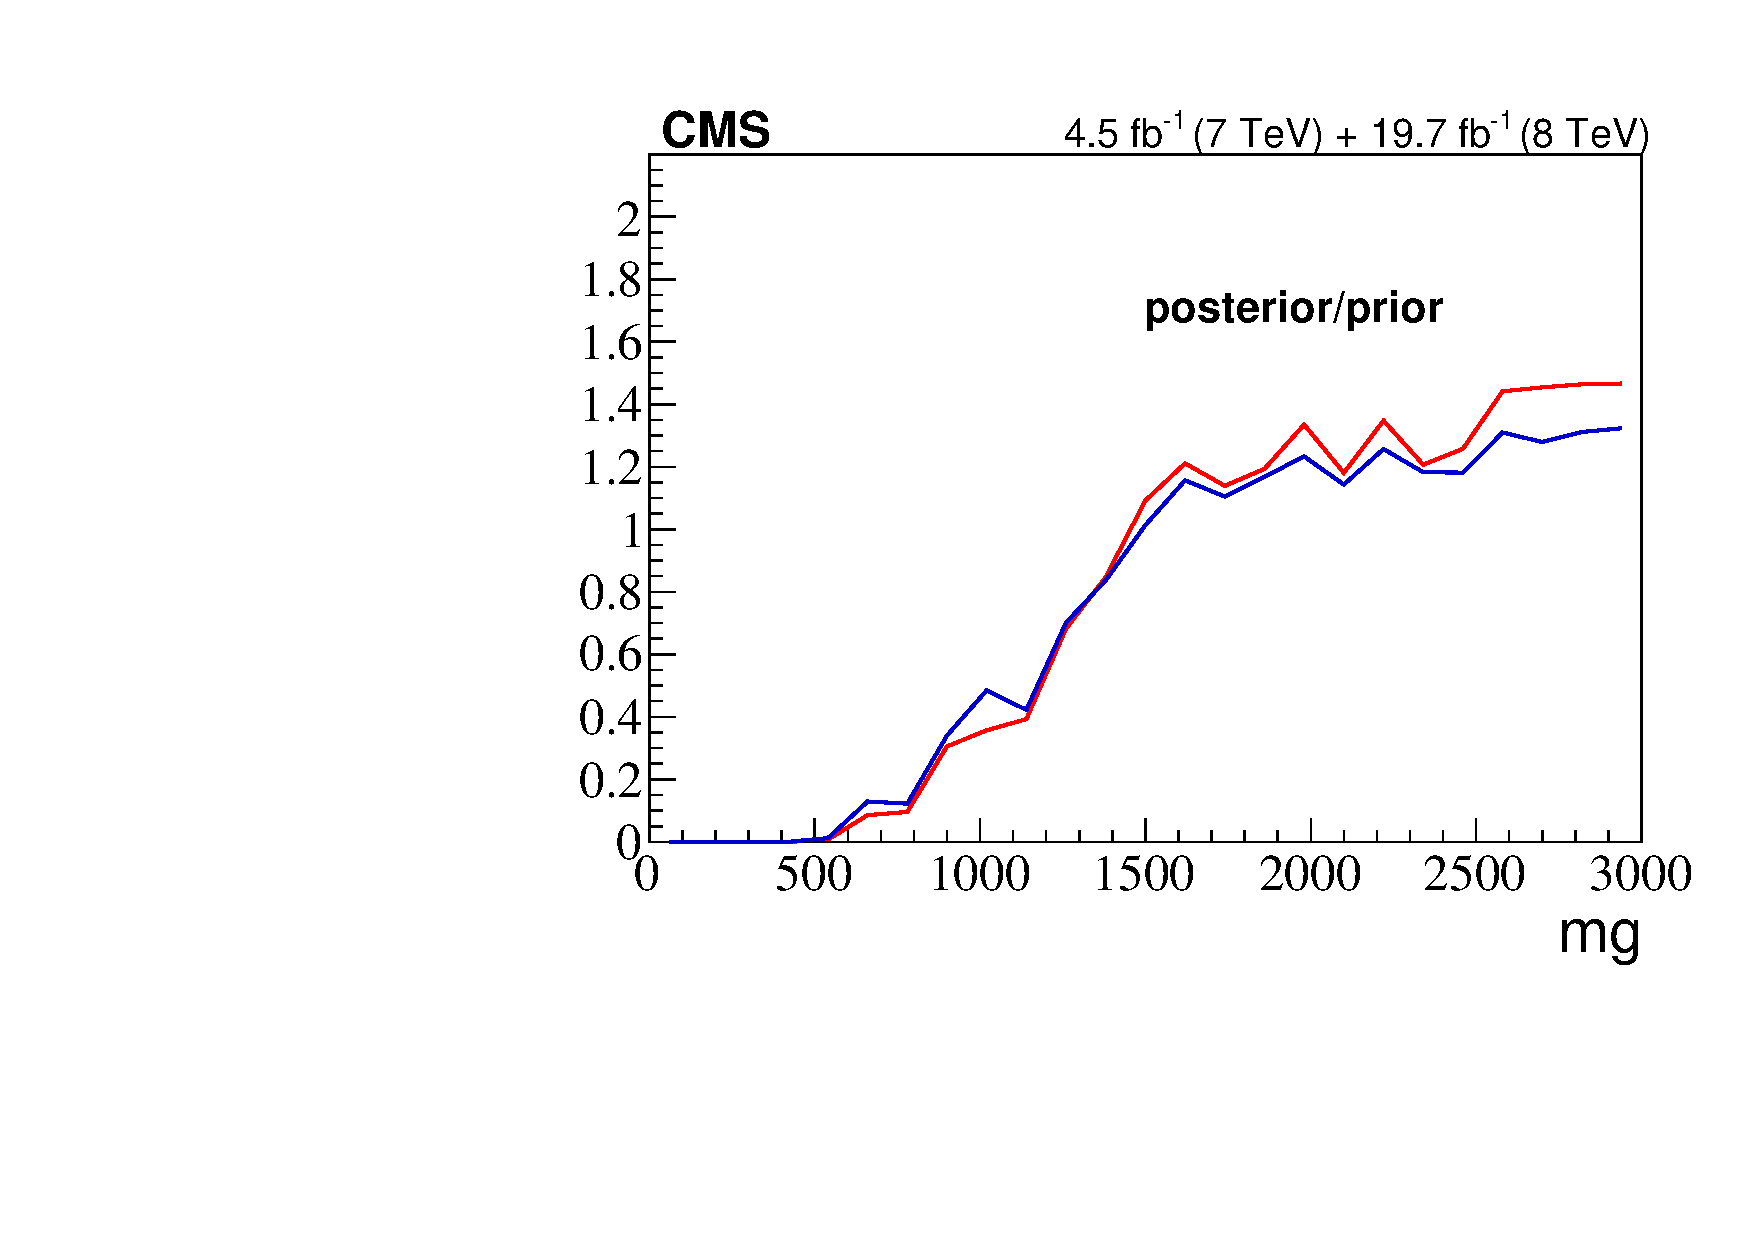
\includegraphics[width=0.5\linewidth]{figures/pMSSMpaper/Prior/mgratio.pdf}
}\\
\subfloat[]{
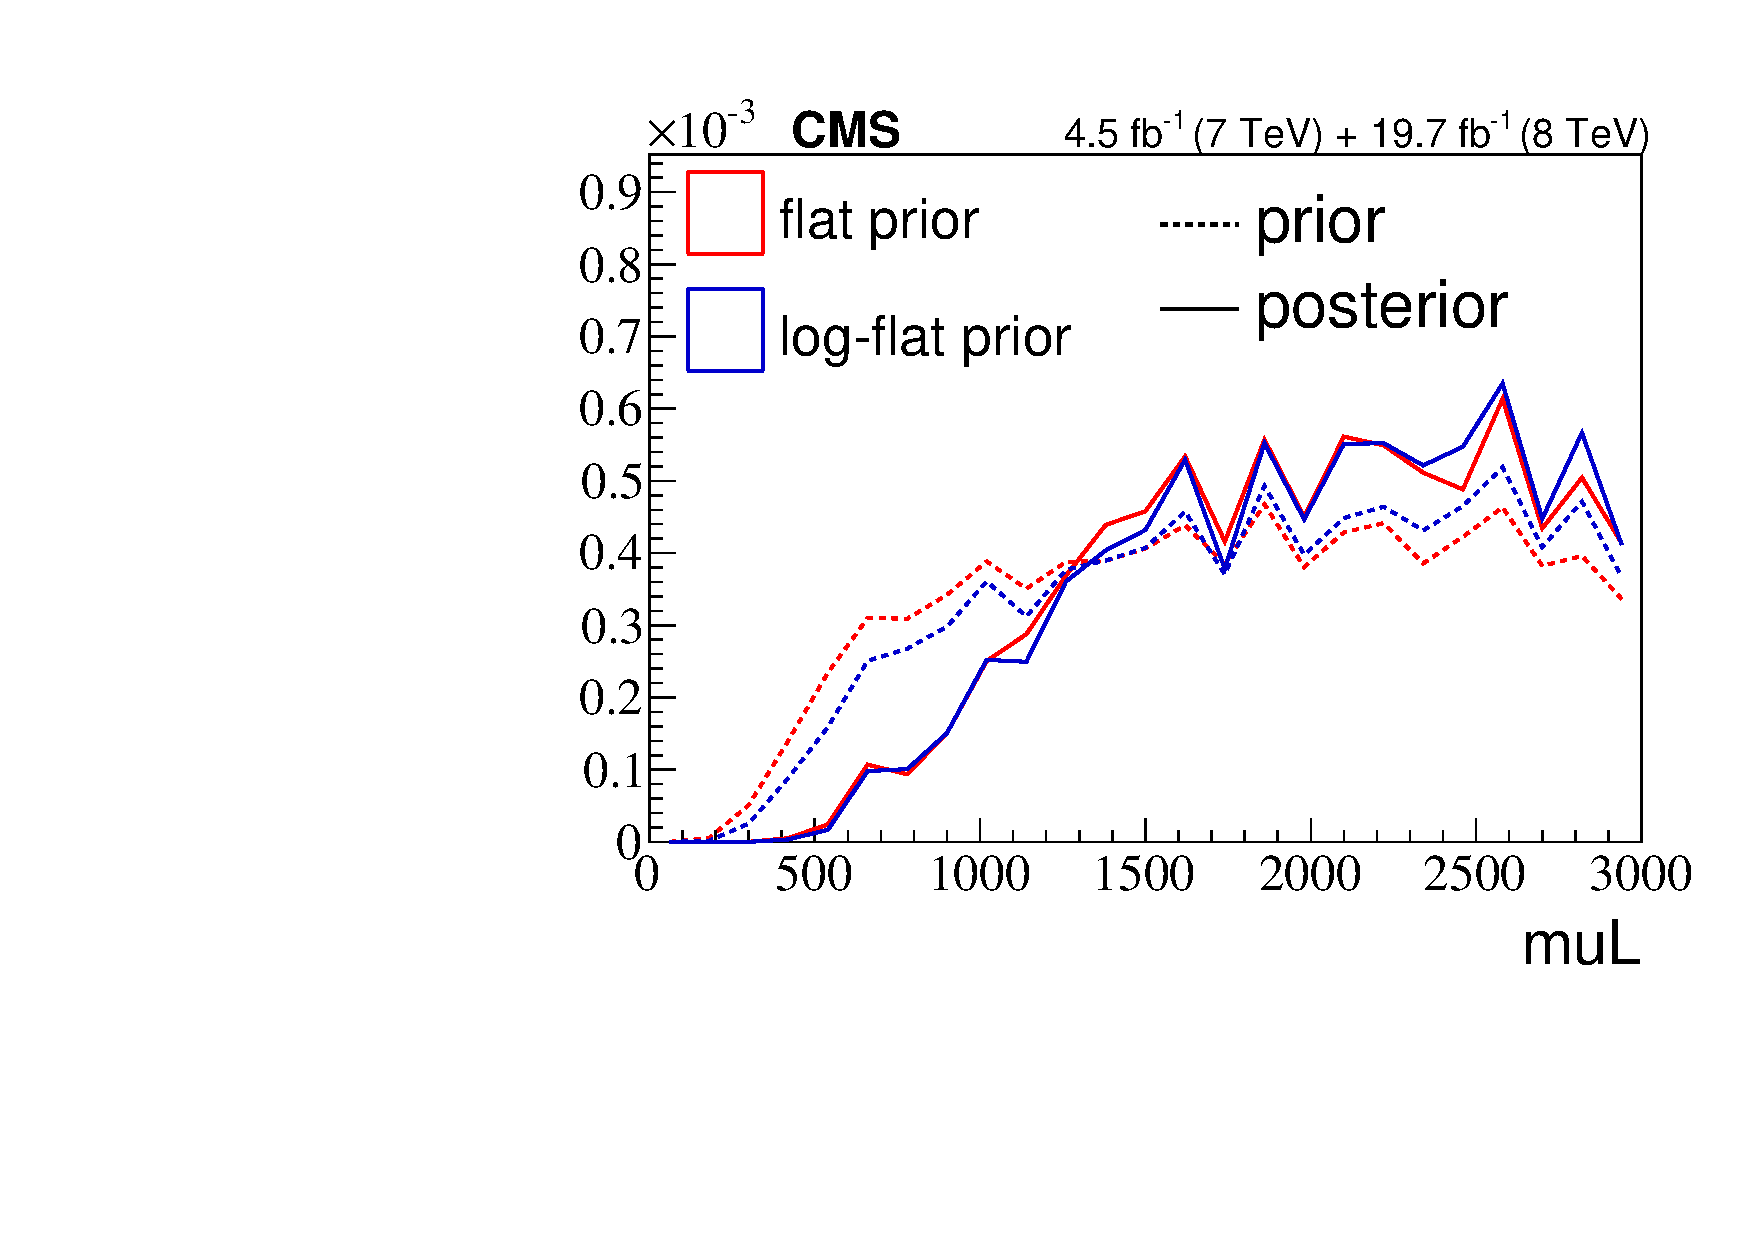
\includegraphics[width=0.5\linewidth]{figures/pMSSMpaper/Prior/muLprepost.pdf}
}
\subfloat[]{
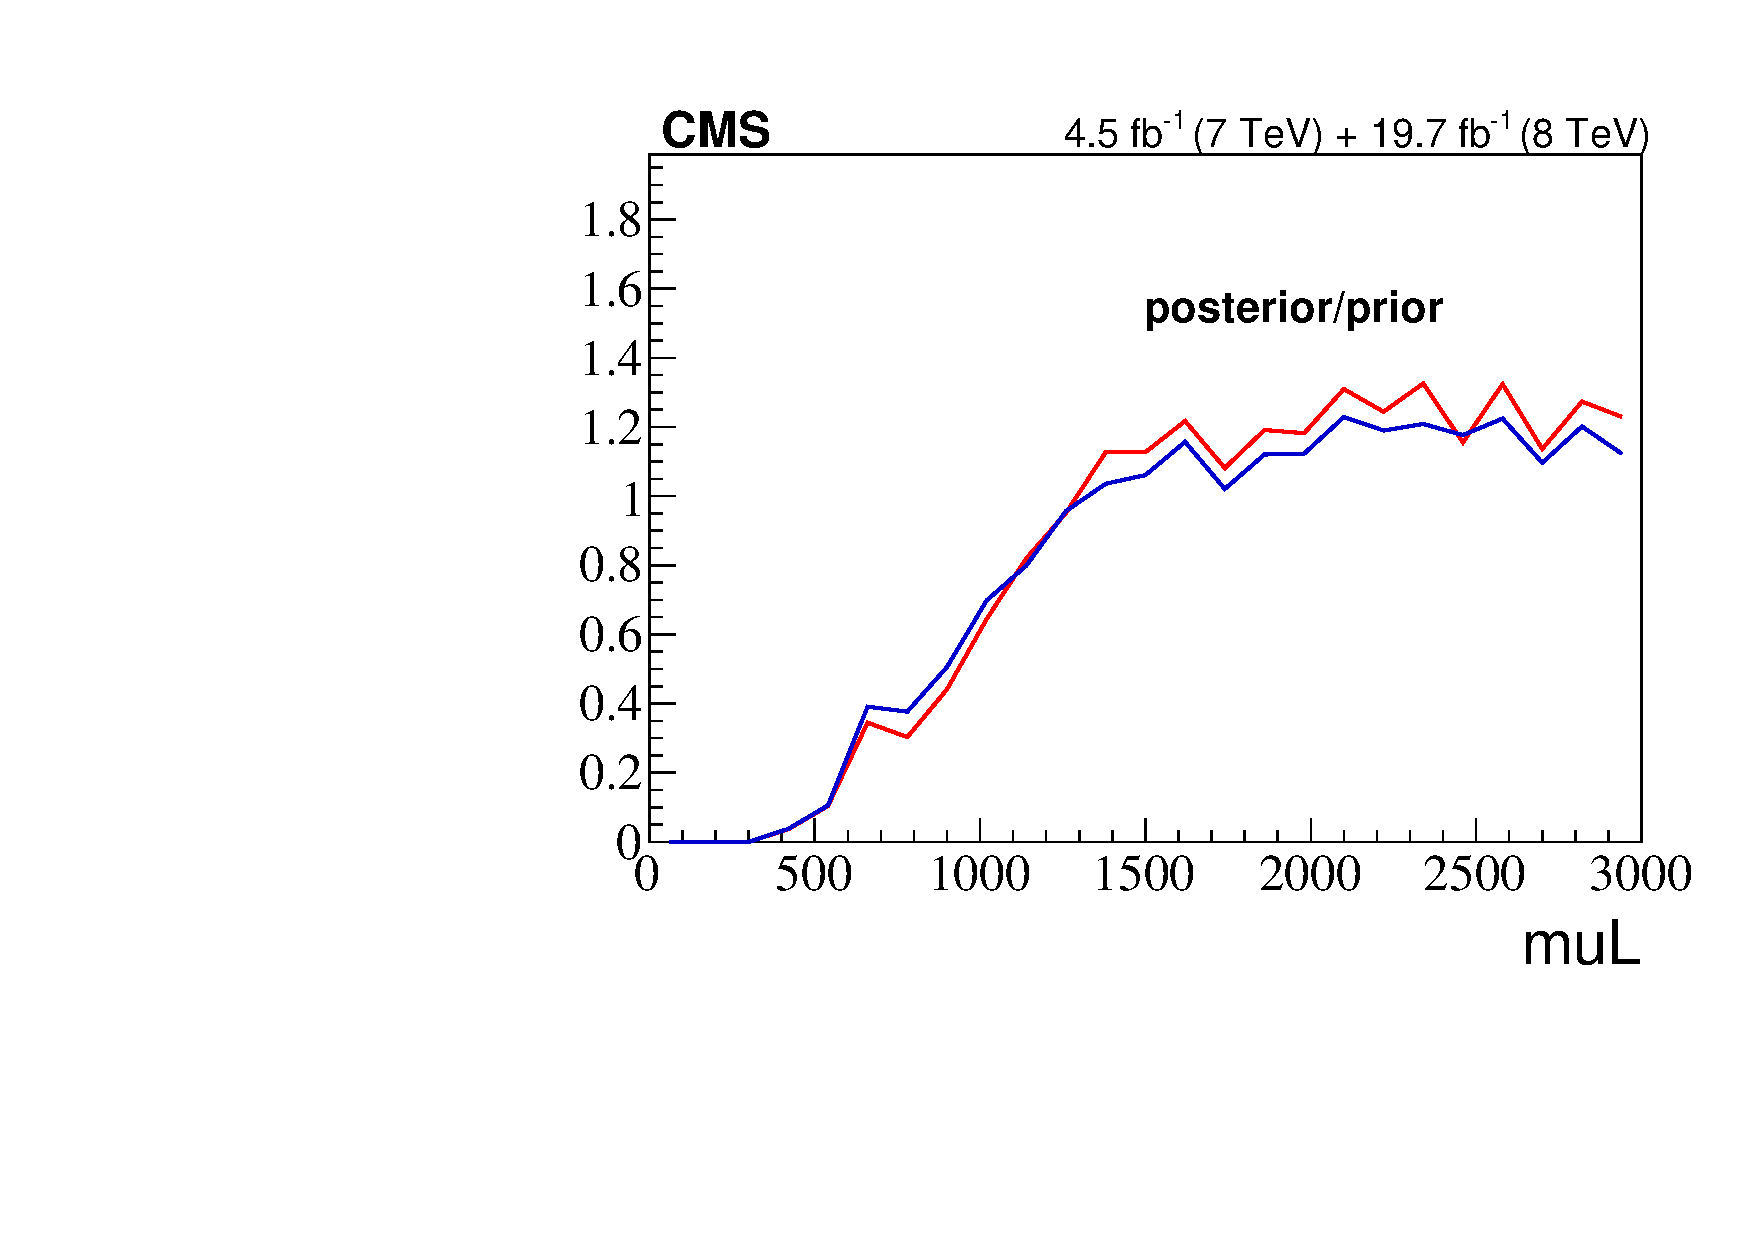
\includegraphics[width=0.5\linewidth]{figures/pMSSMpaper/Prior/muLratio.pdf}

}
\caption{Left: posterior/prior of $m_{\tilde{\text{g}}}$ (top) and $m_{{\text{U}_{\text{L}}}}$ (bottom). Right: Ratio of the posterior to the prior of $m_{\tilde{\text{g}}}$ (top) and $m_{{\text{U}_{\text{L}}}}$ (bottom).}
\label{fig:mg_prepost}
\end{figure}

\begin{figure}[h]
\centering
\subfloat[]{
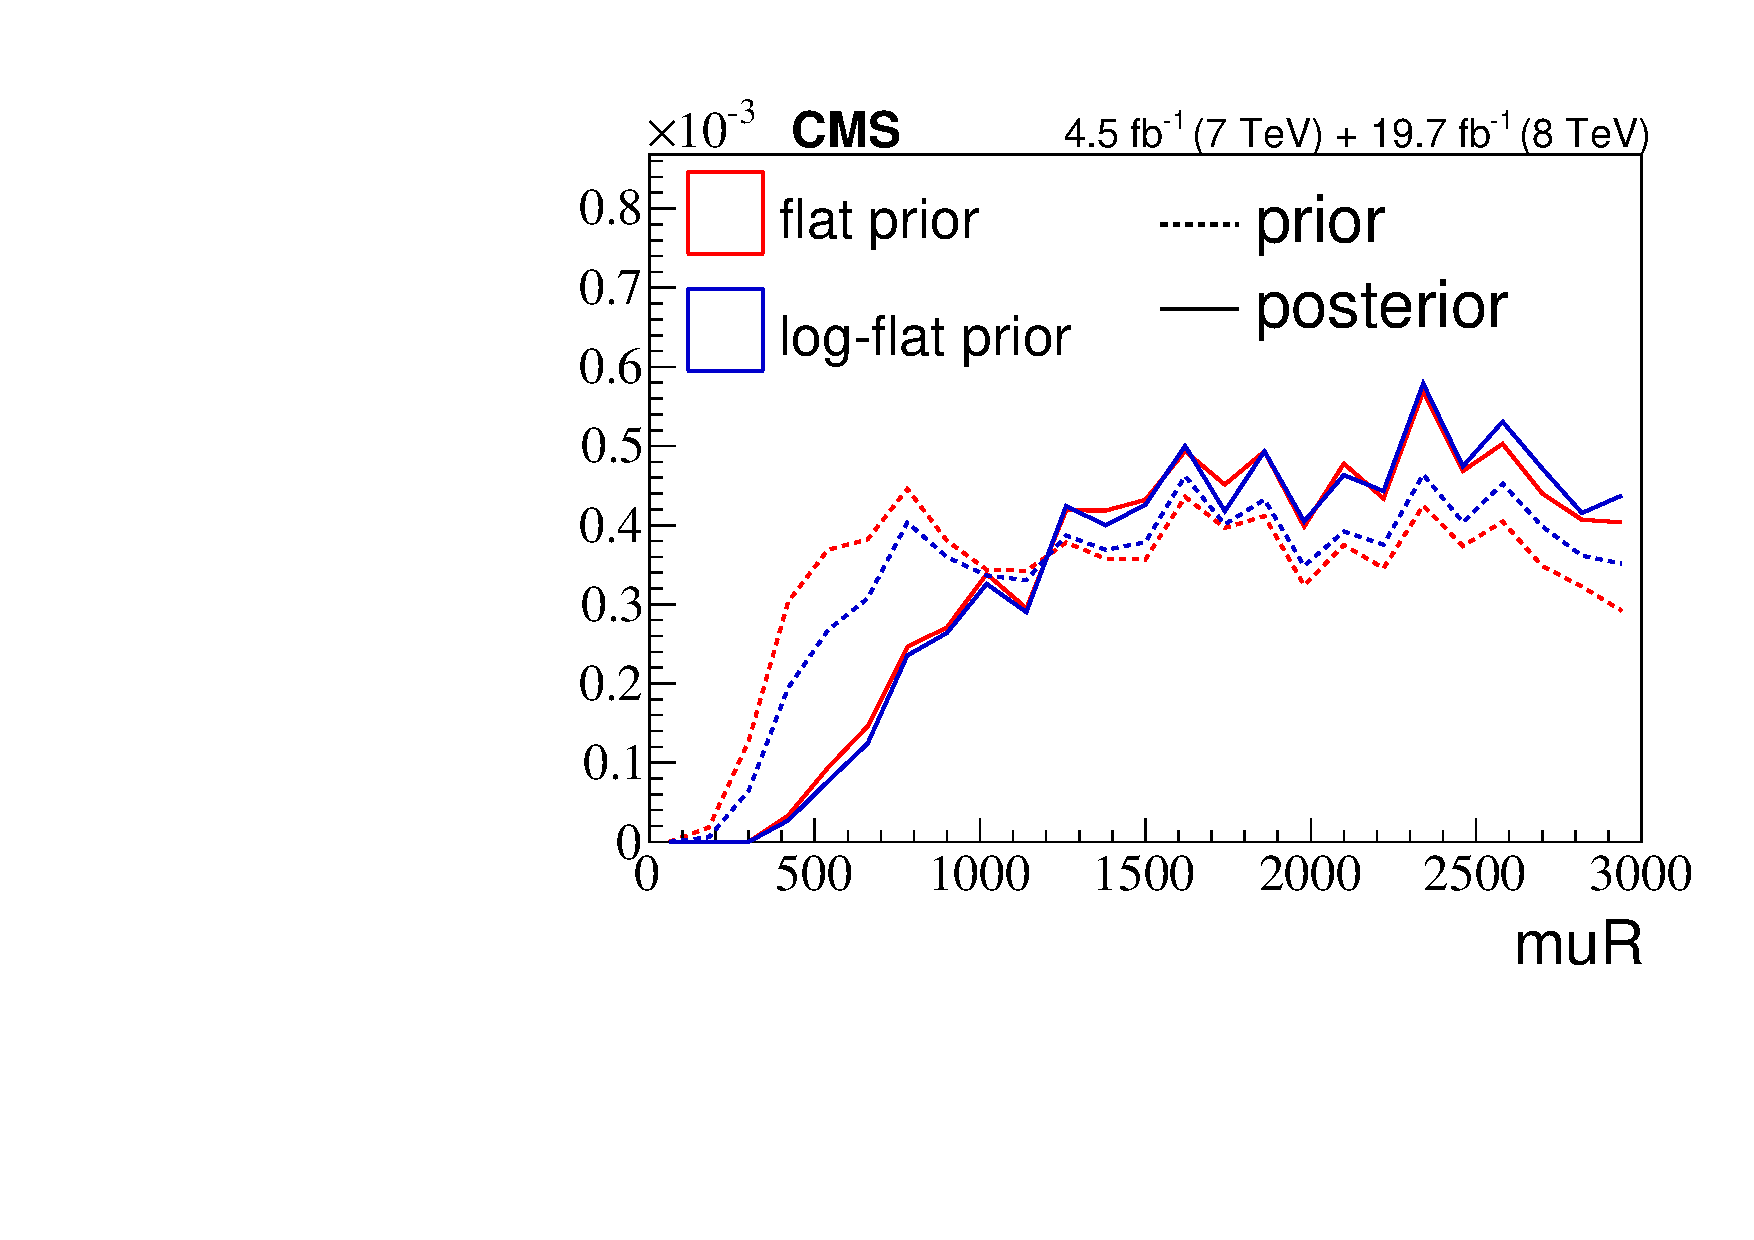
\includegraphics[width=0.5\linewidth]{figures/pMSSMpaper/Prior/muRprepost.pdf}
}
\subfloat[]{
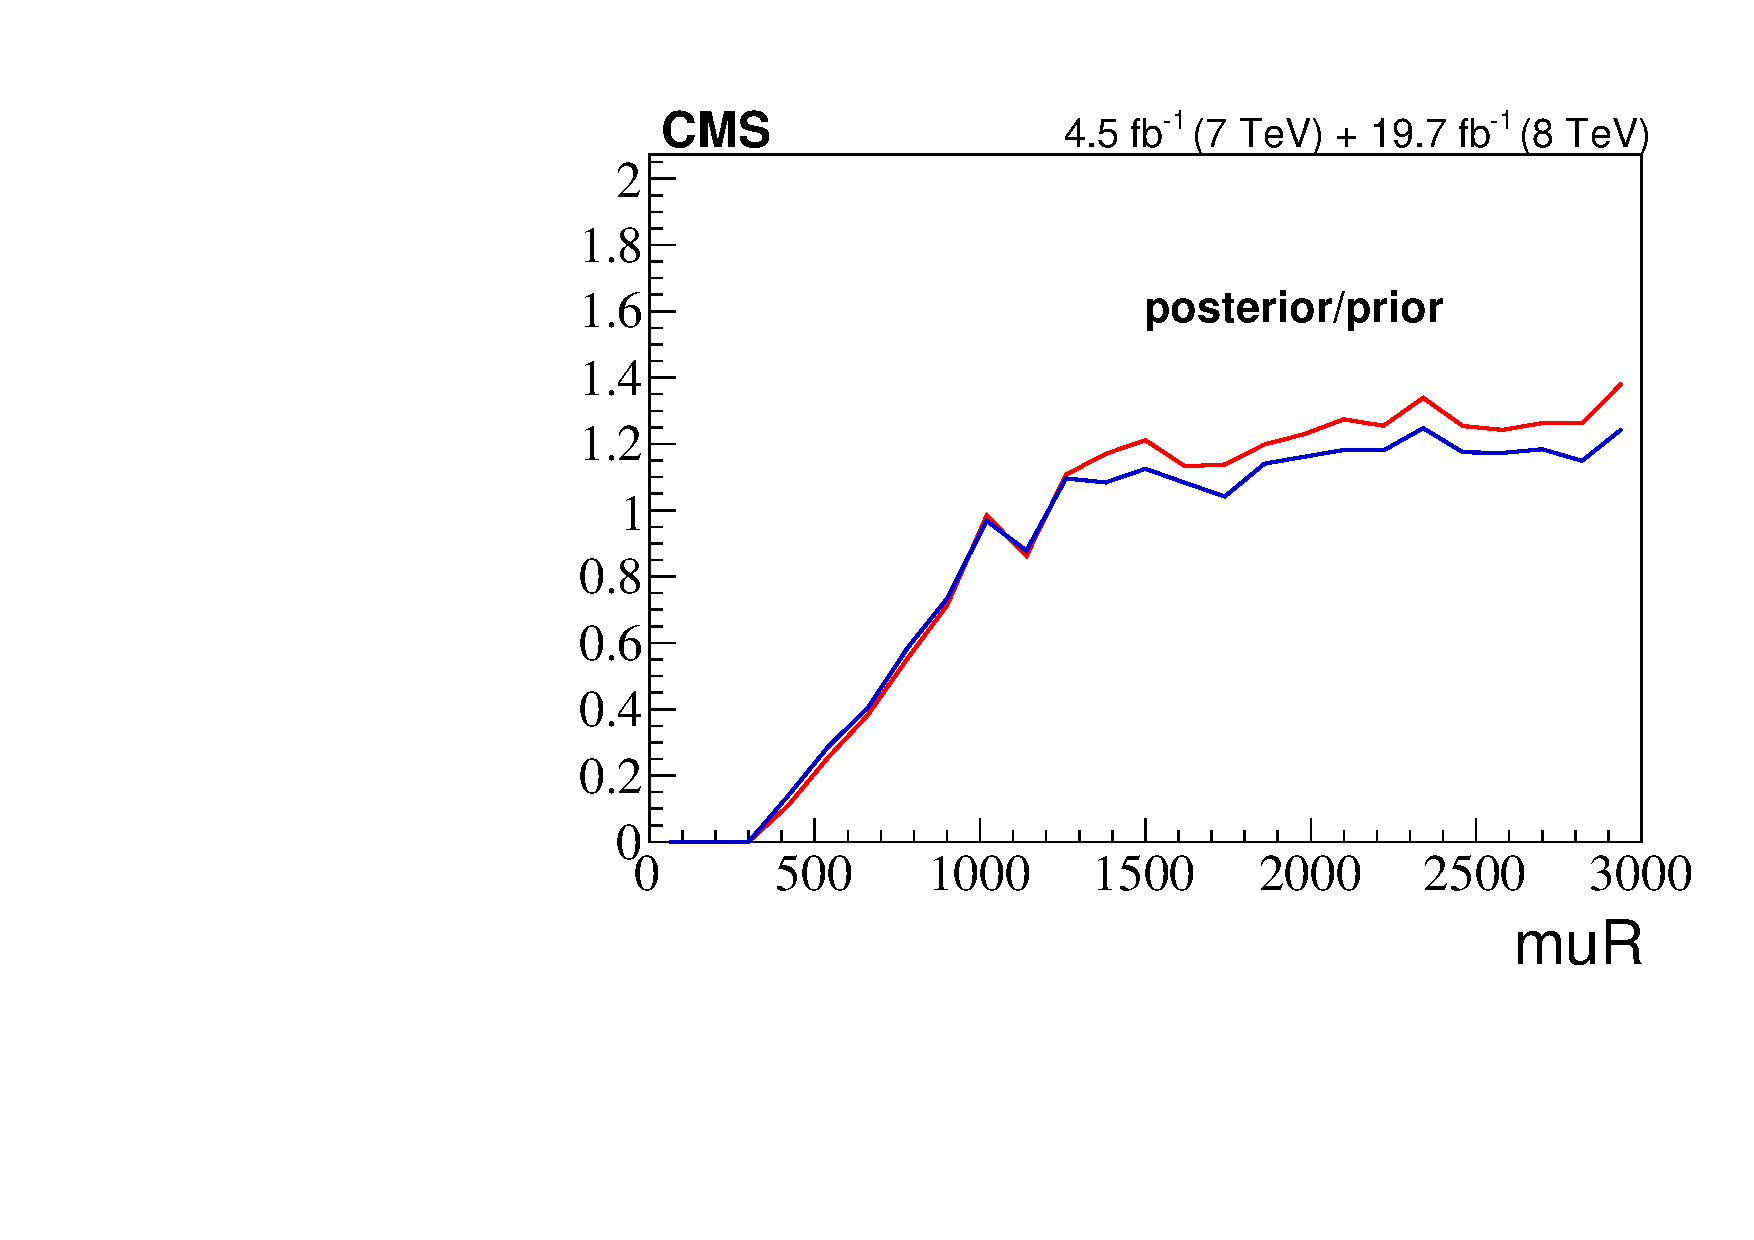
\includegraphics[width=0.5\linewidth]{figures/pMSSMpaper/Prior/muRratio.pdf}
}\\
\subfloat[]{
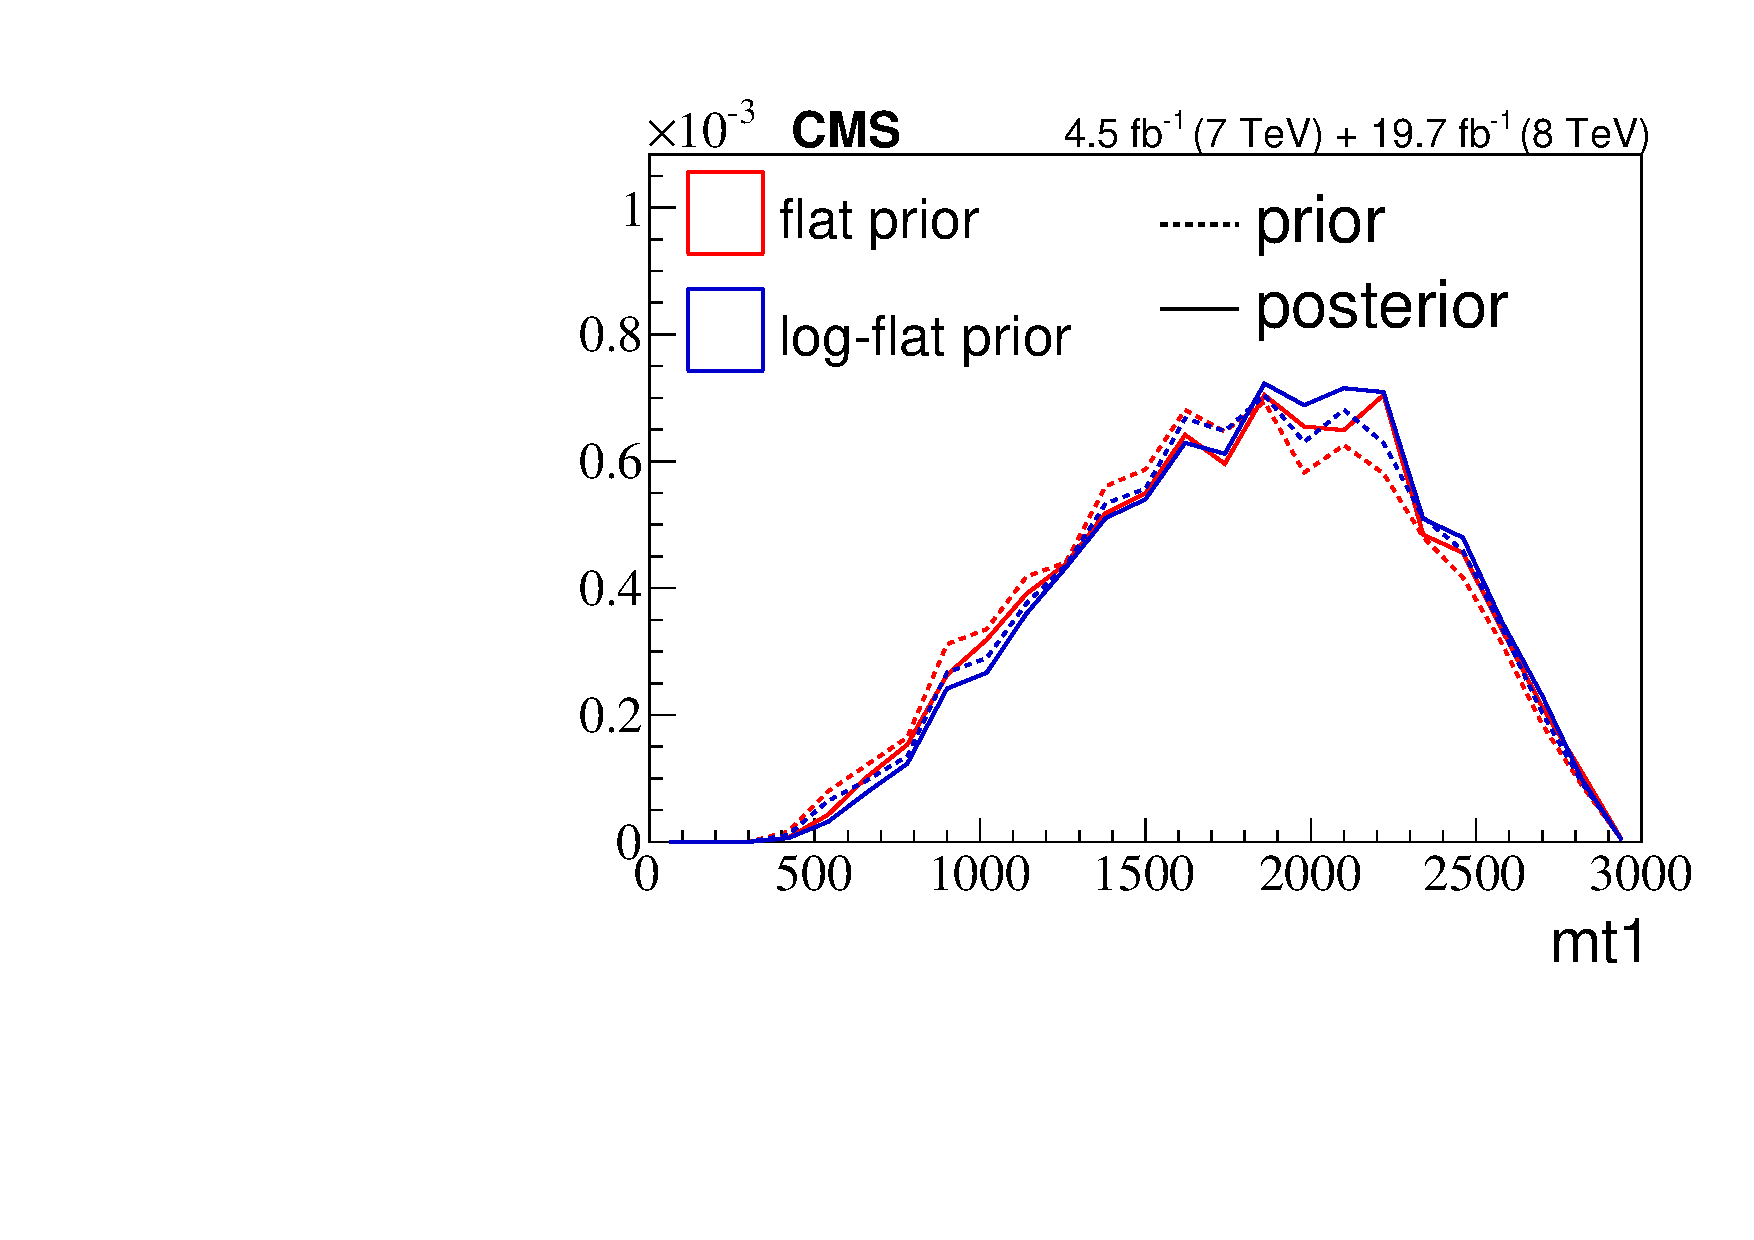
\includegraphics[width=0.5\linewidth]{figures/pMSSMpaper/Prior/mt1prepost.pdf}
}
\subfloat[]{
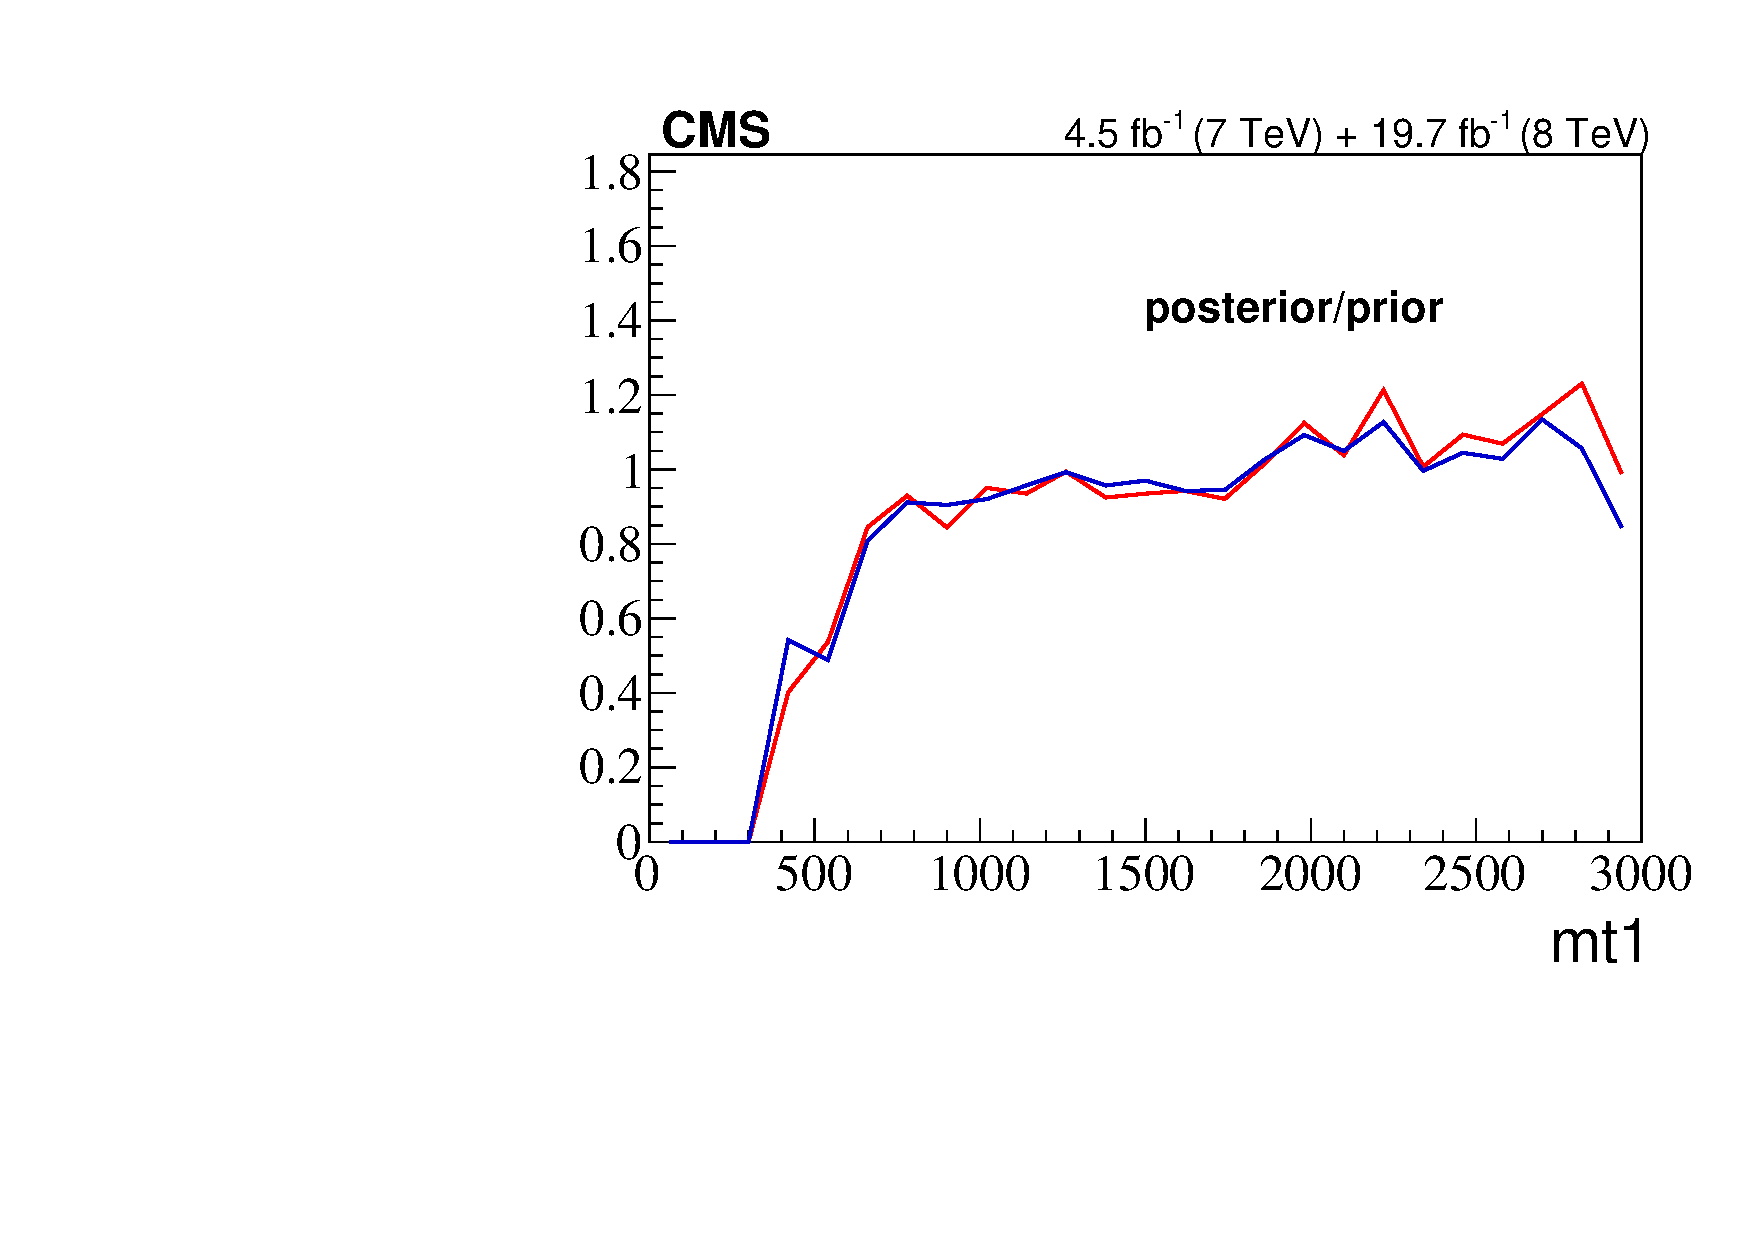
\includegraphics[width=0.5\linewidth]{figures/pMSSMpaper/Prior/mt1ratio.pdf}
}
\caption{Left: posterior/prior of $m_{\text{U}_R}$ (top) and $m_{\tilde{\text{t}}_1}$ (bottom). Right: Ratio of the posterior to the prior of $m_{\text{U}_R}$ (top) and $m_{\tilde{\text{t}}_1}$ (bottom).}
\label{fig:mApole}
\end{figure}


\begin{figure}[h]
\centering
\subfloat[]{
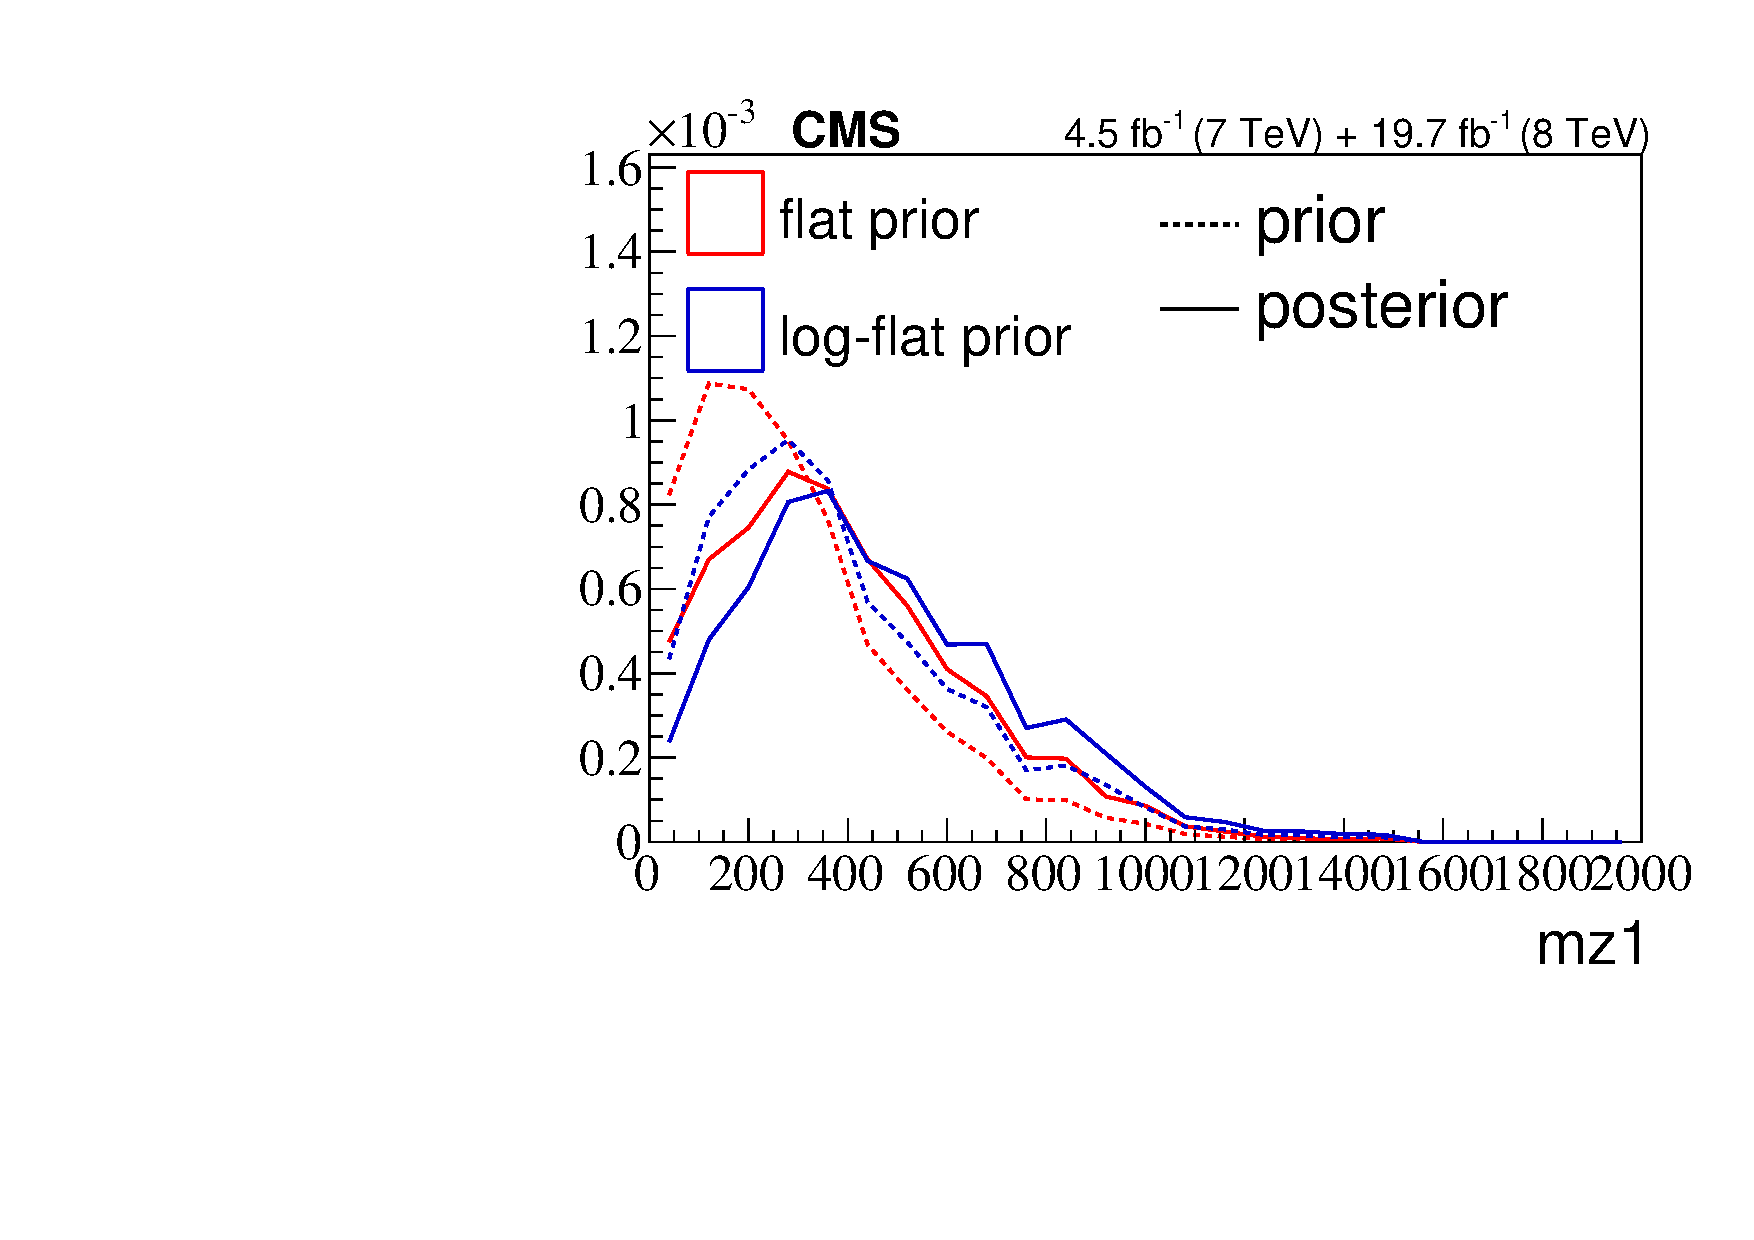
\includegraphics[width=0.5\linewidth]{figures/pMSSMpaper/Prior/mz1prepost.pdf}
}
\subfloat[]{
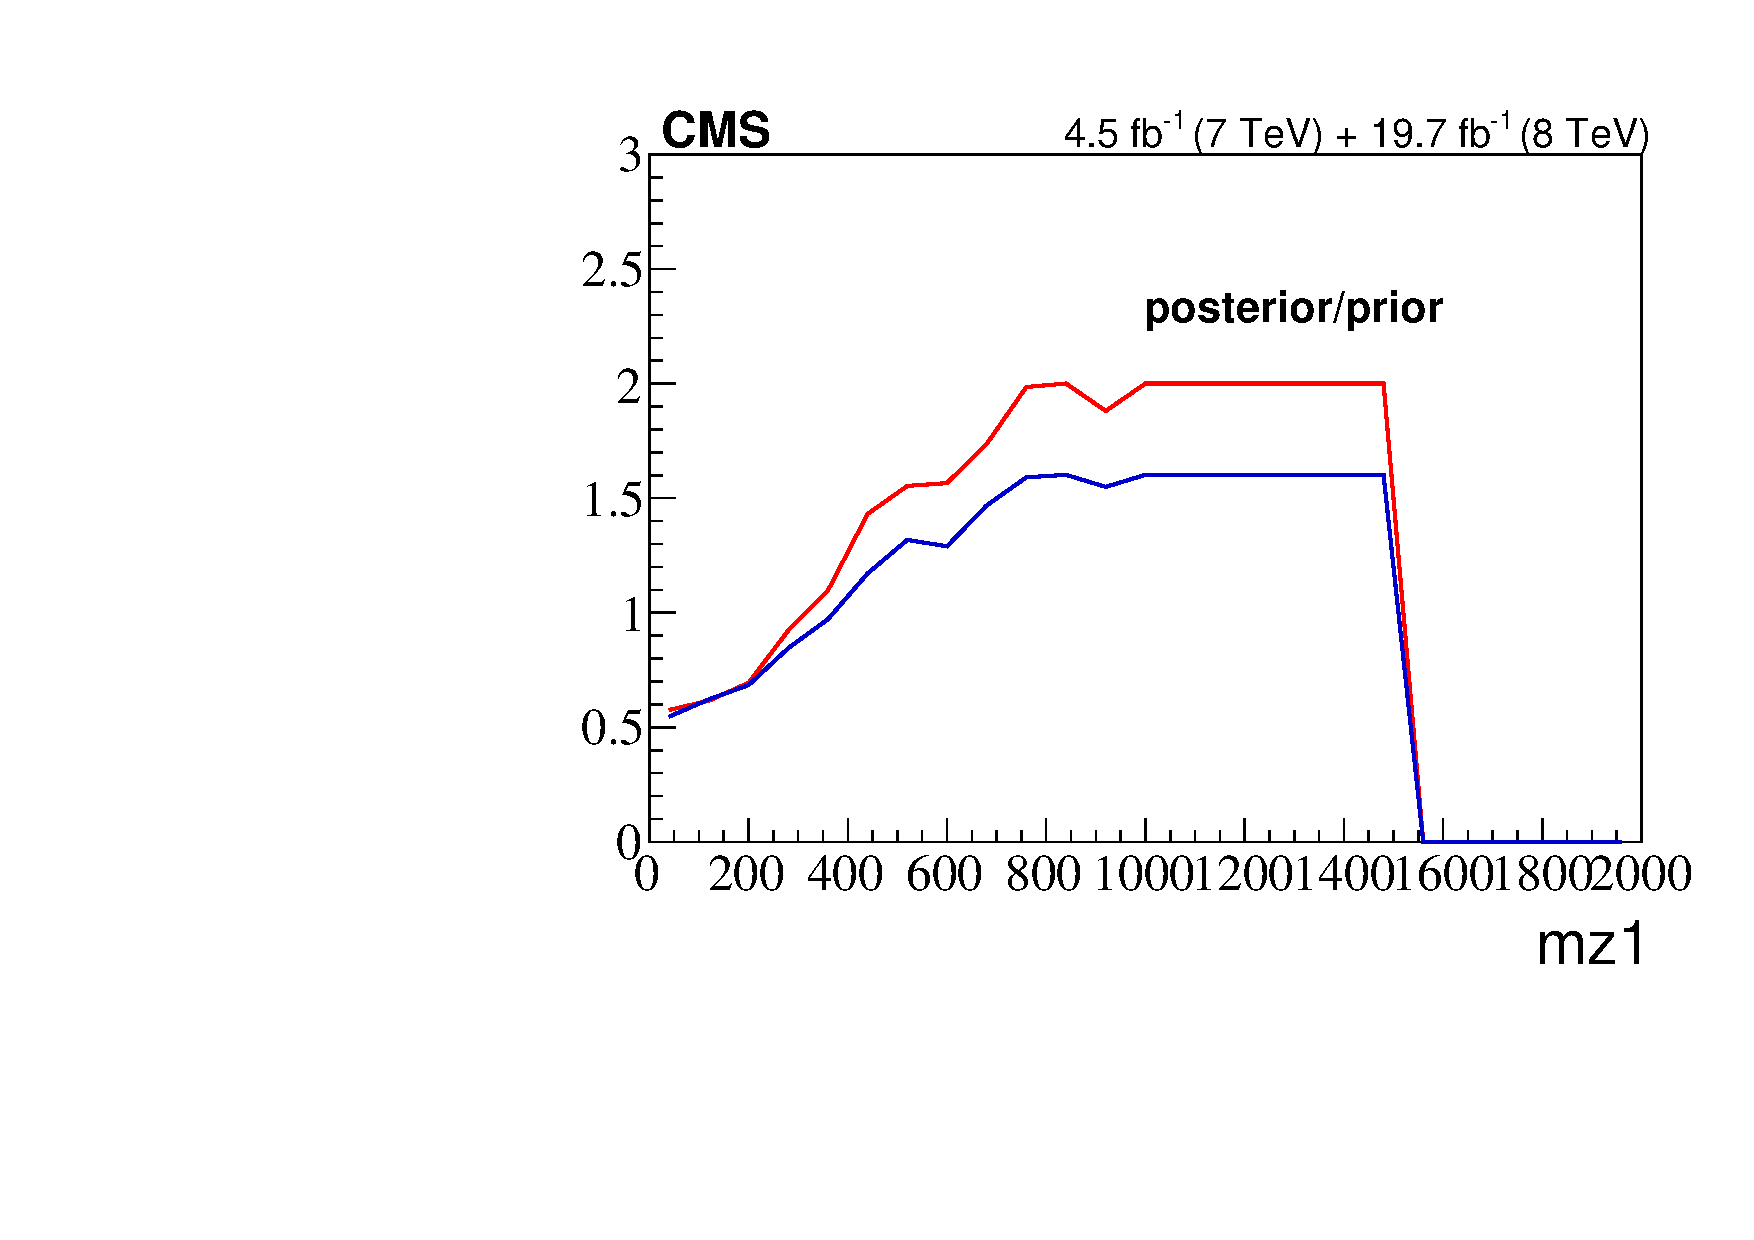
\includegraphics[width=0.5\linewidth]{figures/pMSSMpaper/Prior/mz1ratio.pdf}
}\\
\subfloat[]{
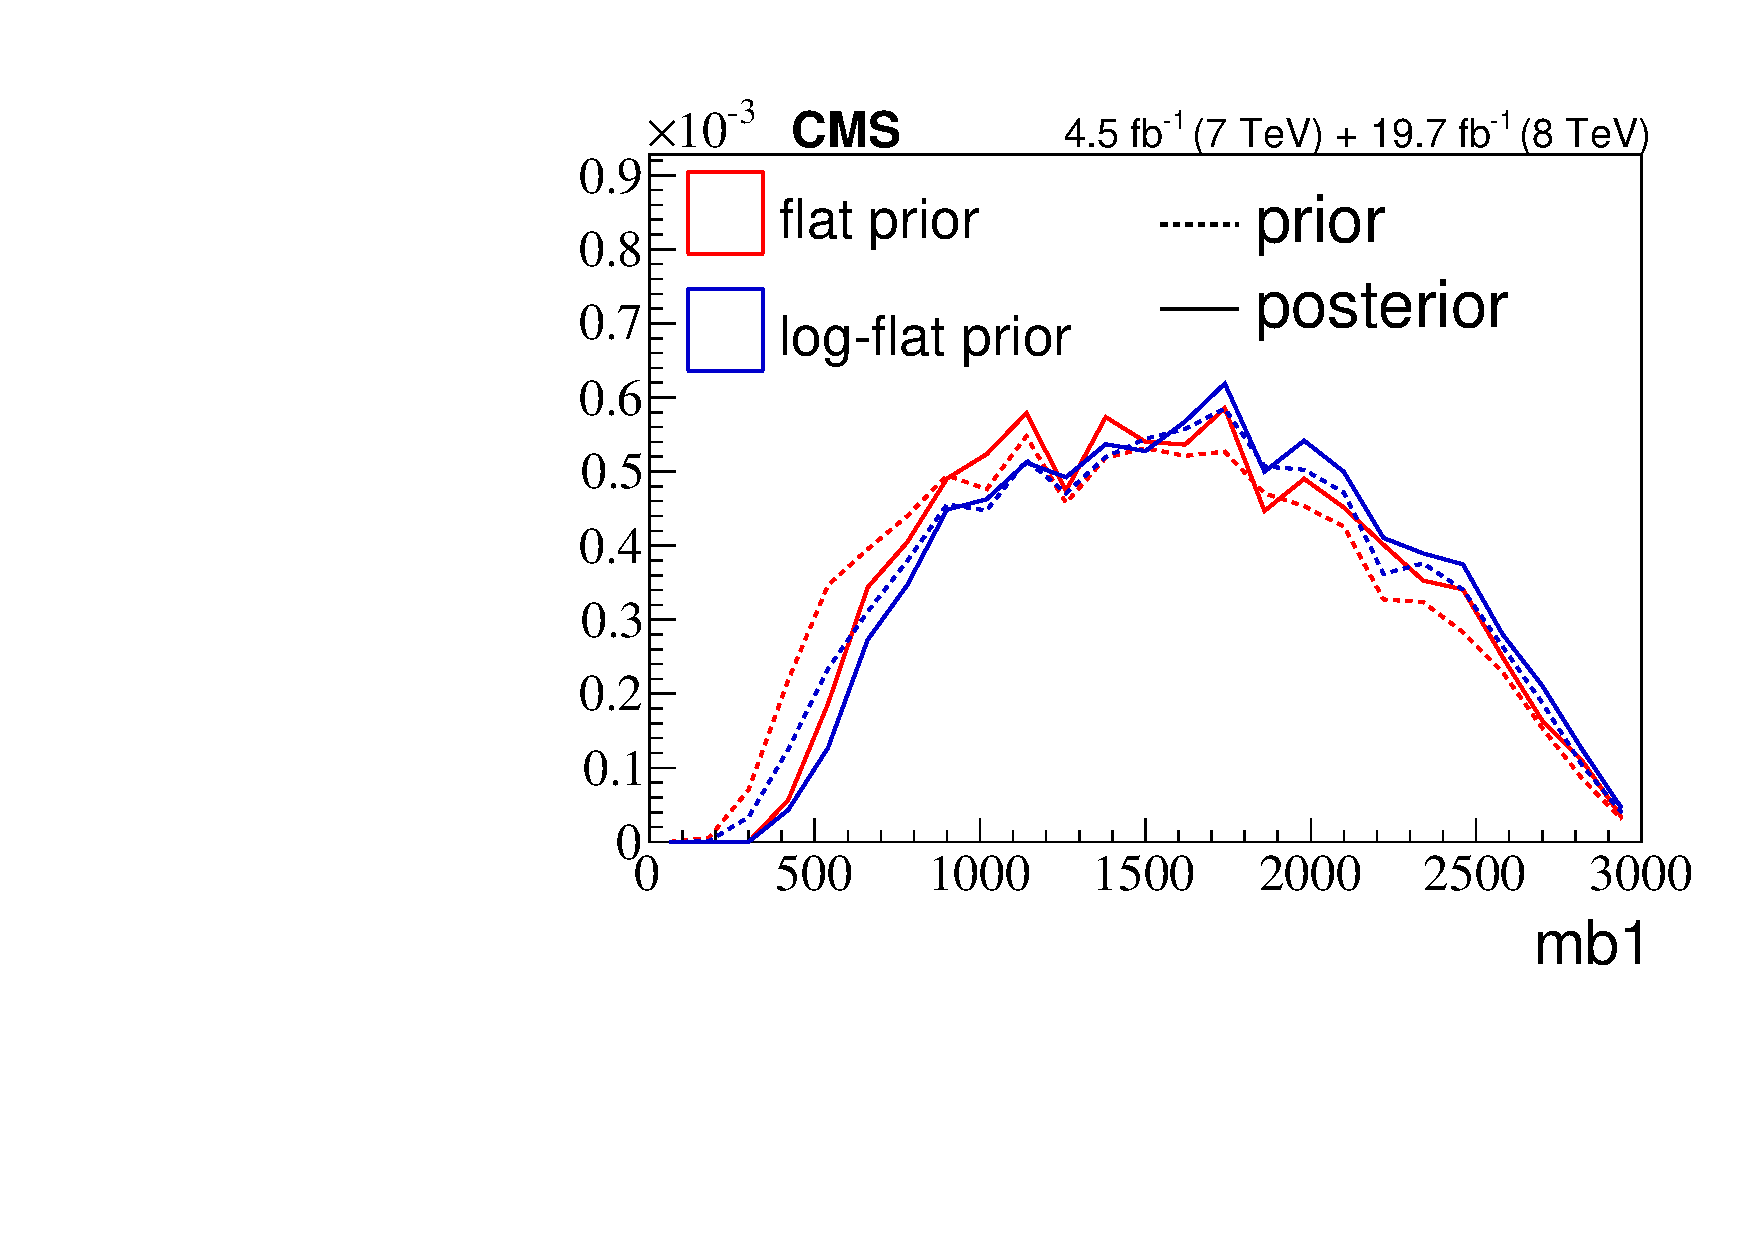
\includegraphics[width=0.5\linewidth]{figures/pMSSMpaper/Prior/mb1prepost.pdf}
}
\subfloat[]{
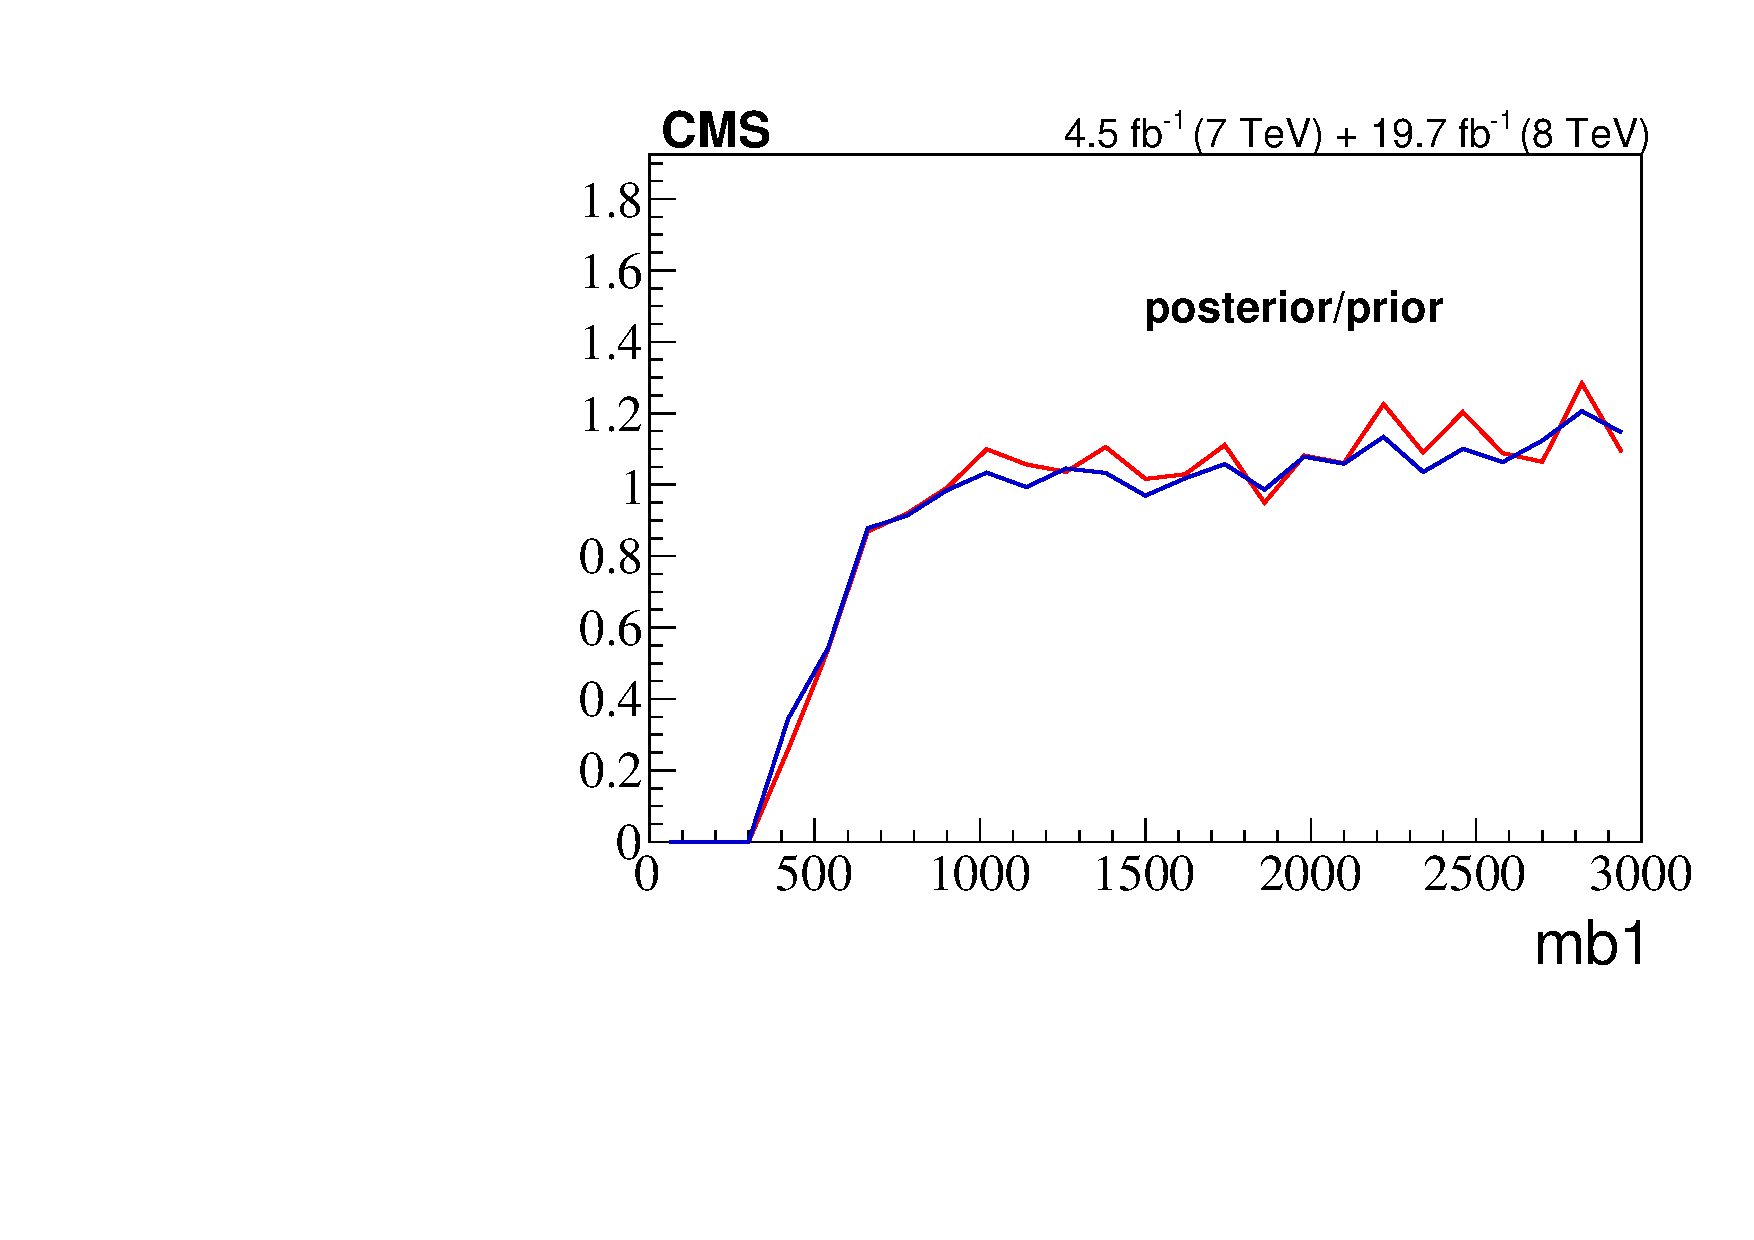
\includegraphics[width=0.5\linewidth]{figures/pMSSMpaper/Prior/mb1ratio.pdf}

}
\caption{Left: posterior/prior of $m_{\tilde{\chi}^{0}_{1}}$ (top) and $m_{\tilde{\text{b}}_1}$ (bottom). Right: Ratio of the posterior to the prior of $m_{\chi^{0}_{1}}$ (top) and $m_{\tilde{\text{b}}_1}$ (bottom).}
\label{fig:mb1ratio}
\end{figure}
\FloatBarrier

\begin{figure}[h]
\centering
\subfloat[]{
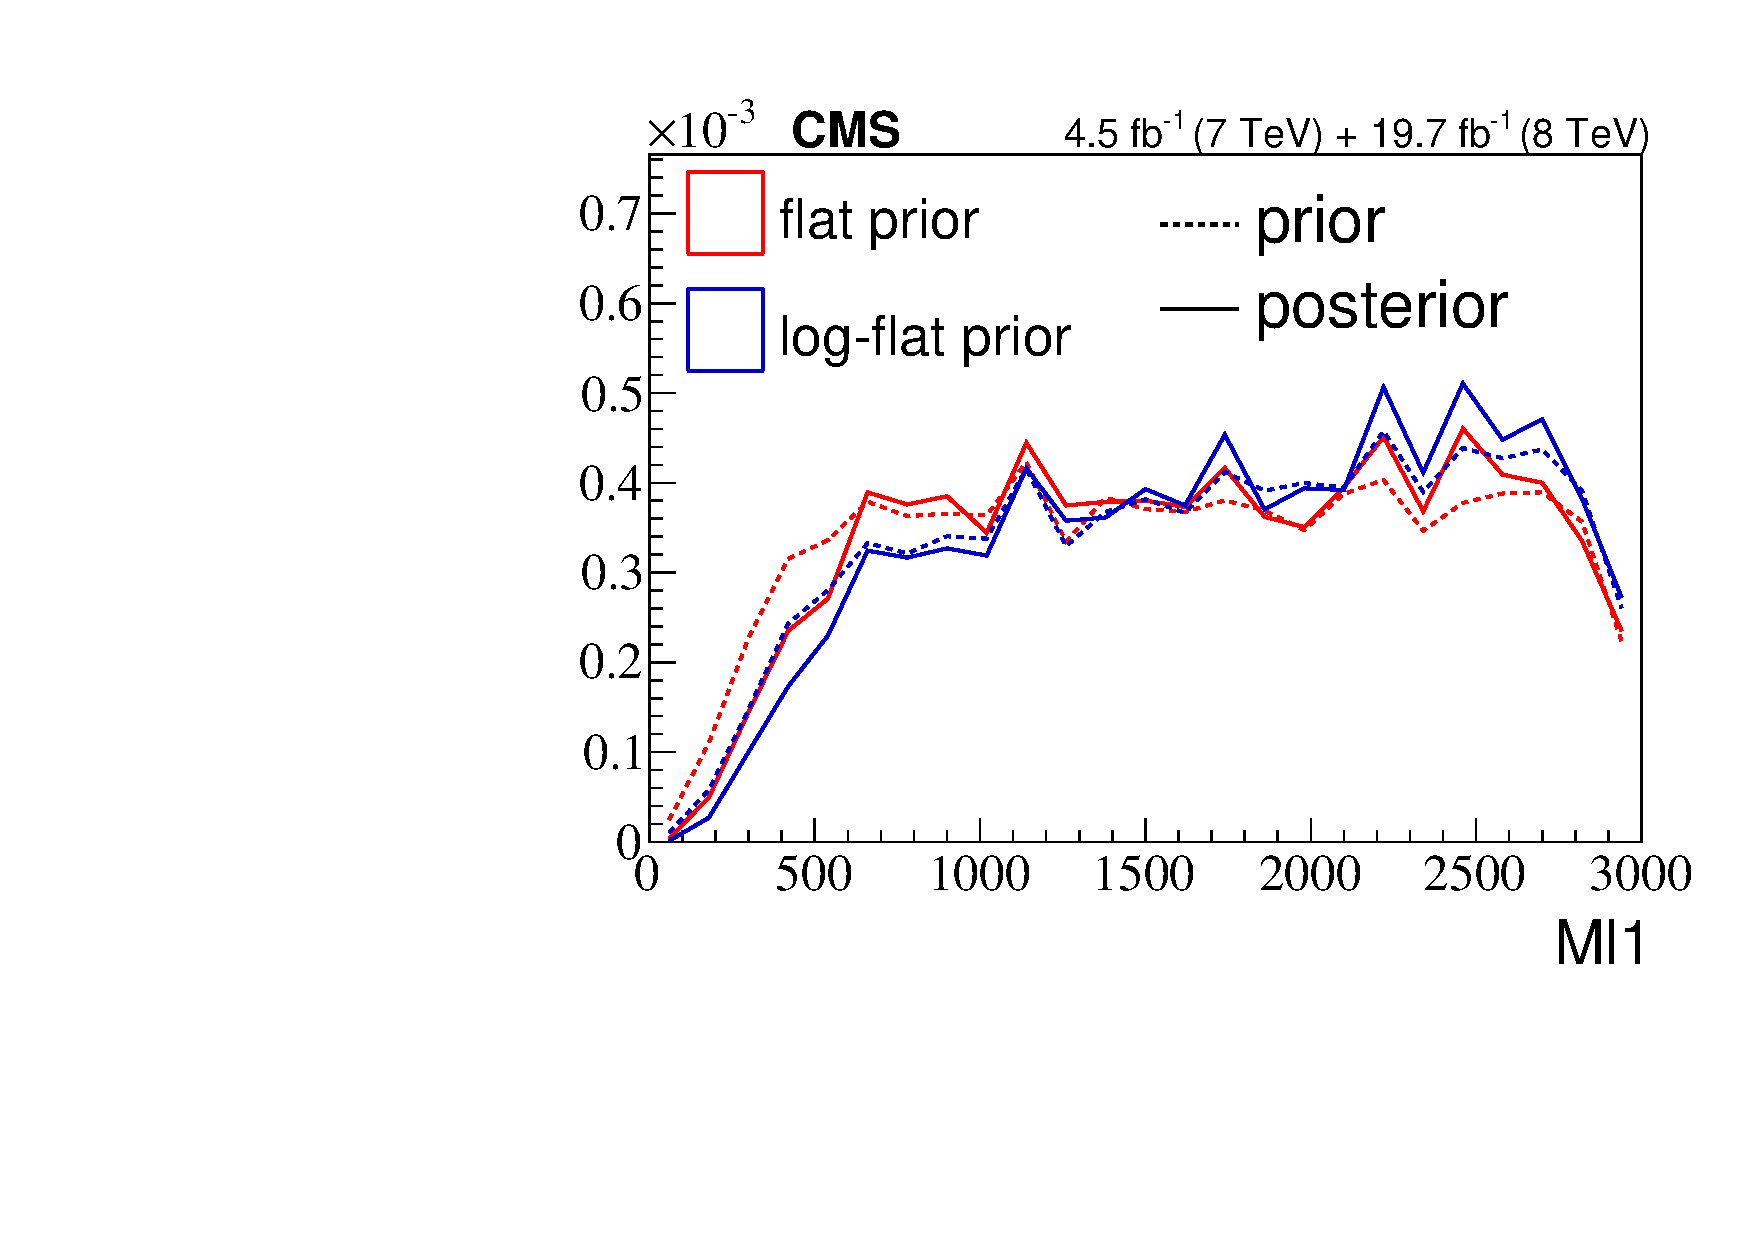
\includegraphics[width=0.5\linewidth]{figures/pMSSMpaper/Prior/Ml1prepost.pdf}
}
\subfloat[]{
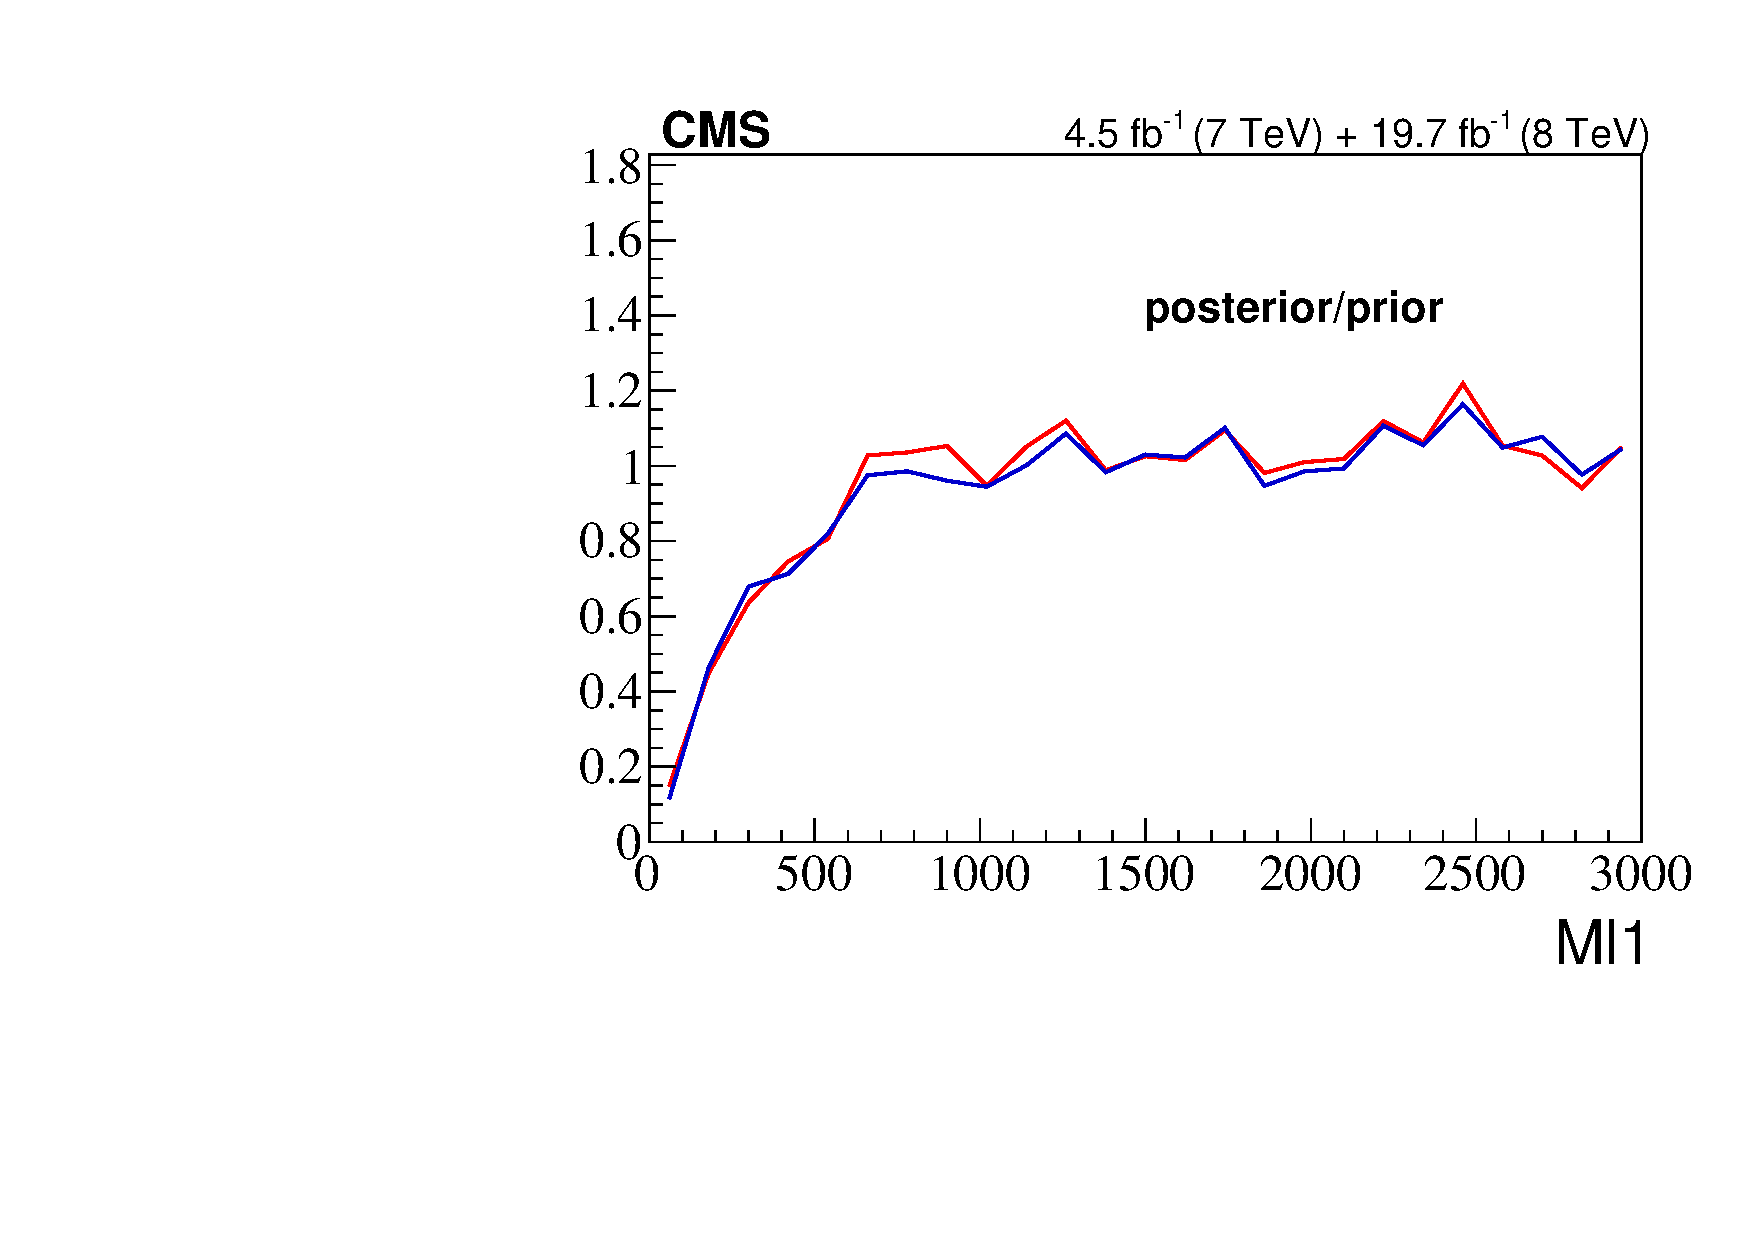
\includegraphics[width=0.5\linewidth]{figures/pMSSMpaper/Prior/Ml1ratio.pdf}
}\\
\subfloat[]{
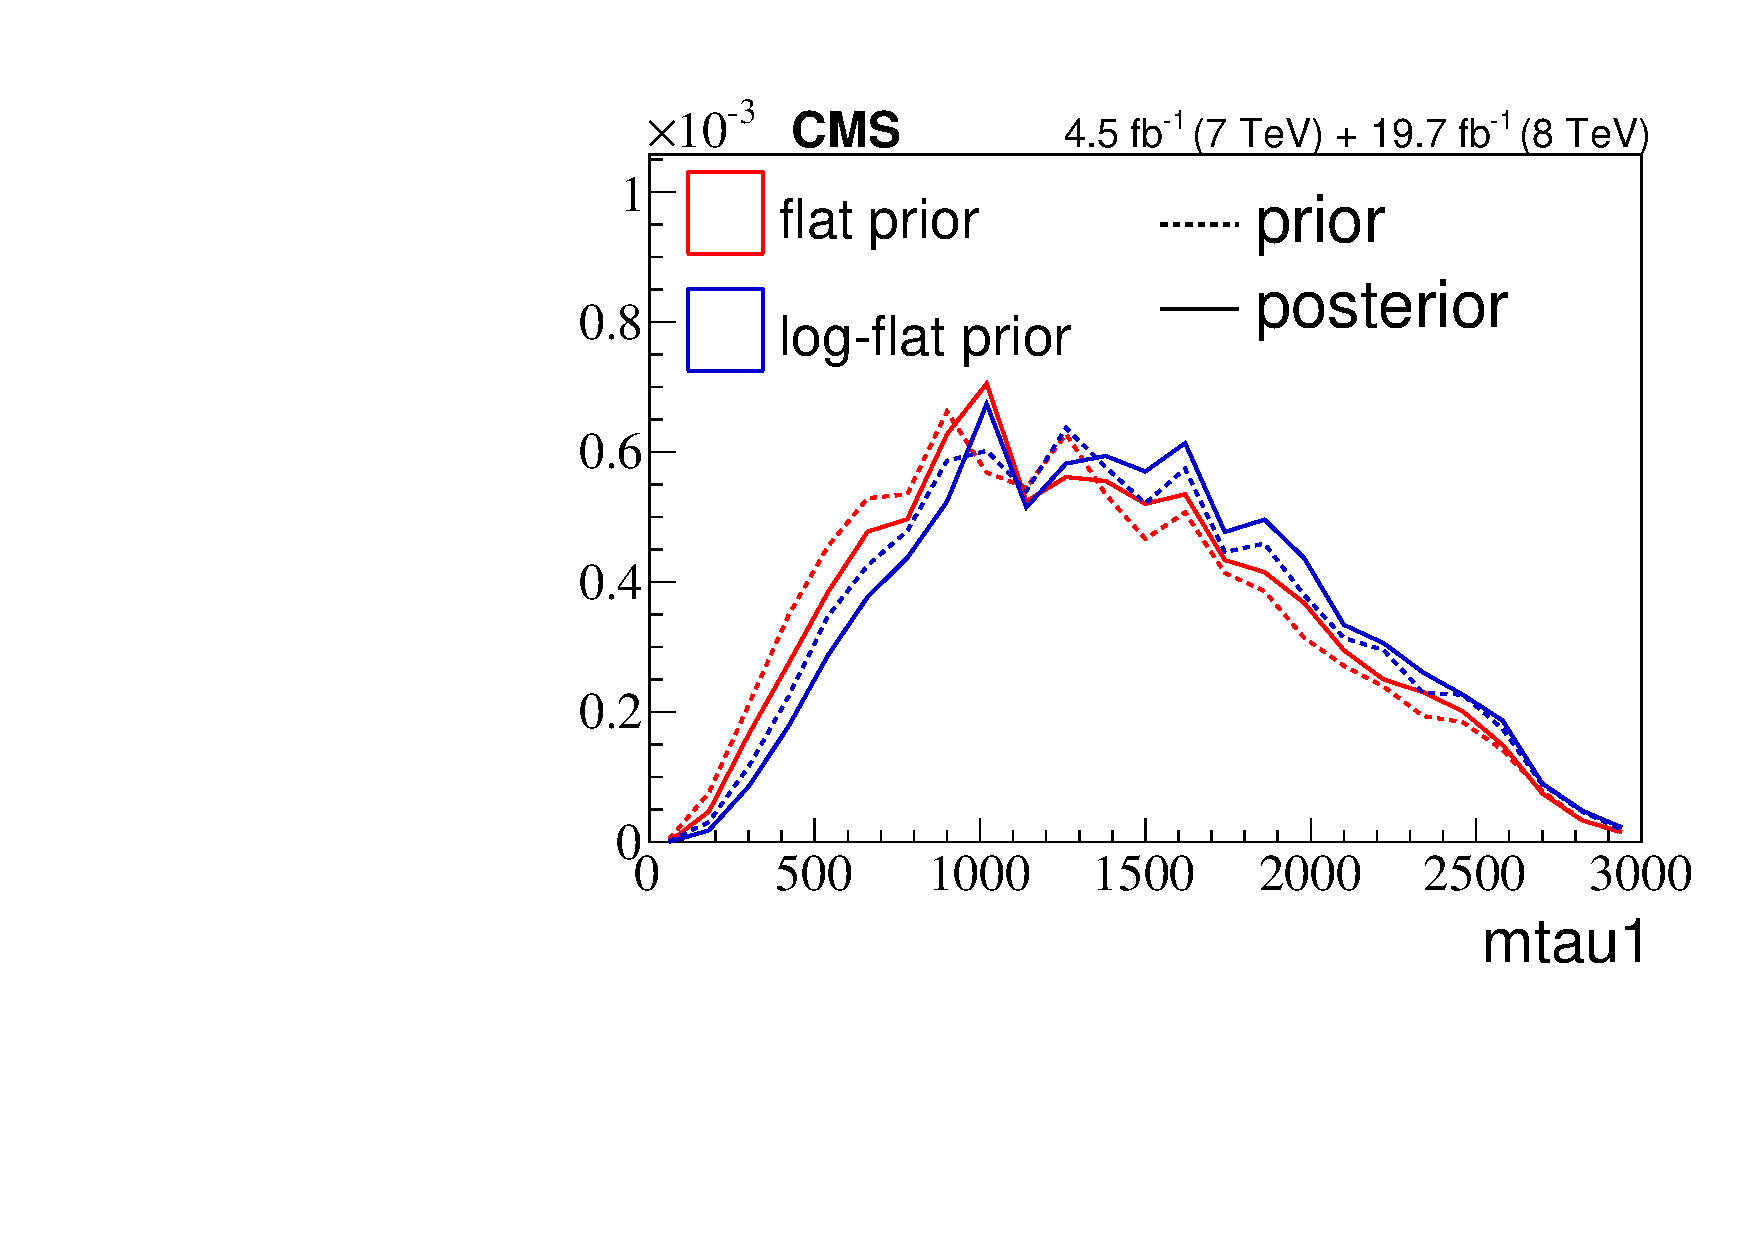
\includegraphics[width=0.5\linewidth]{figures/pMSSMpaper/Prior/mtau1prepost.pdf}
}
\subfloat[]{
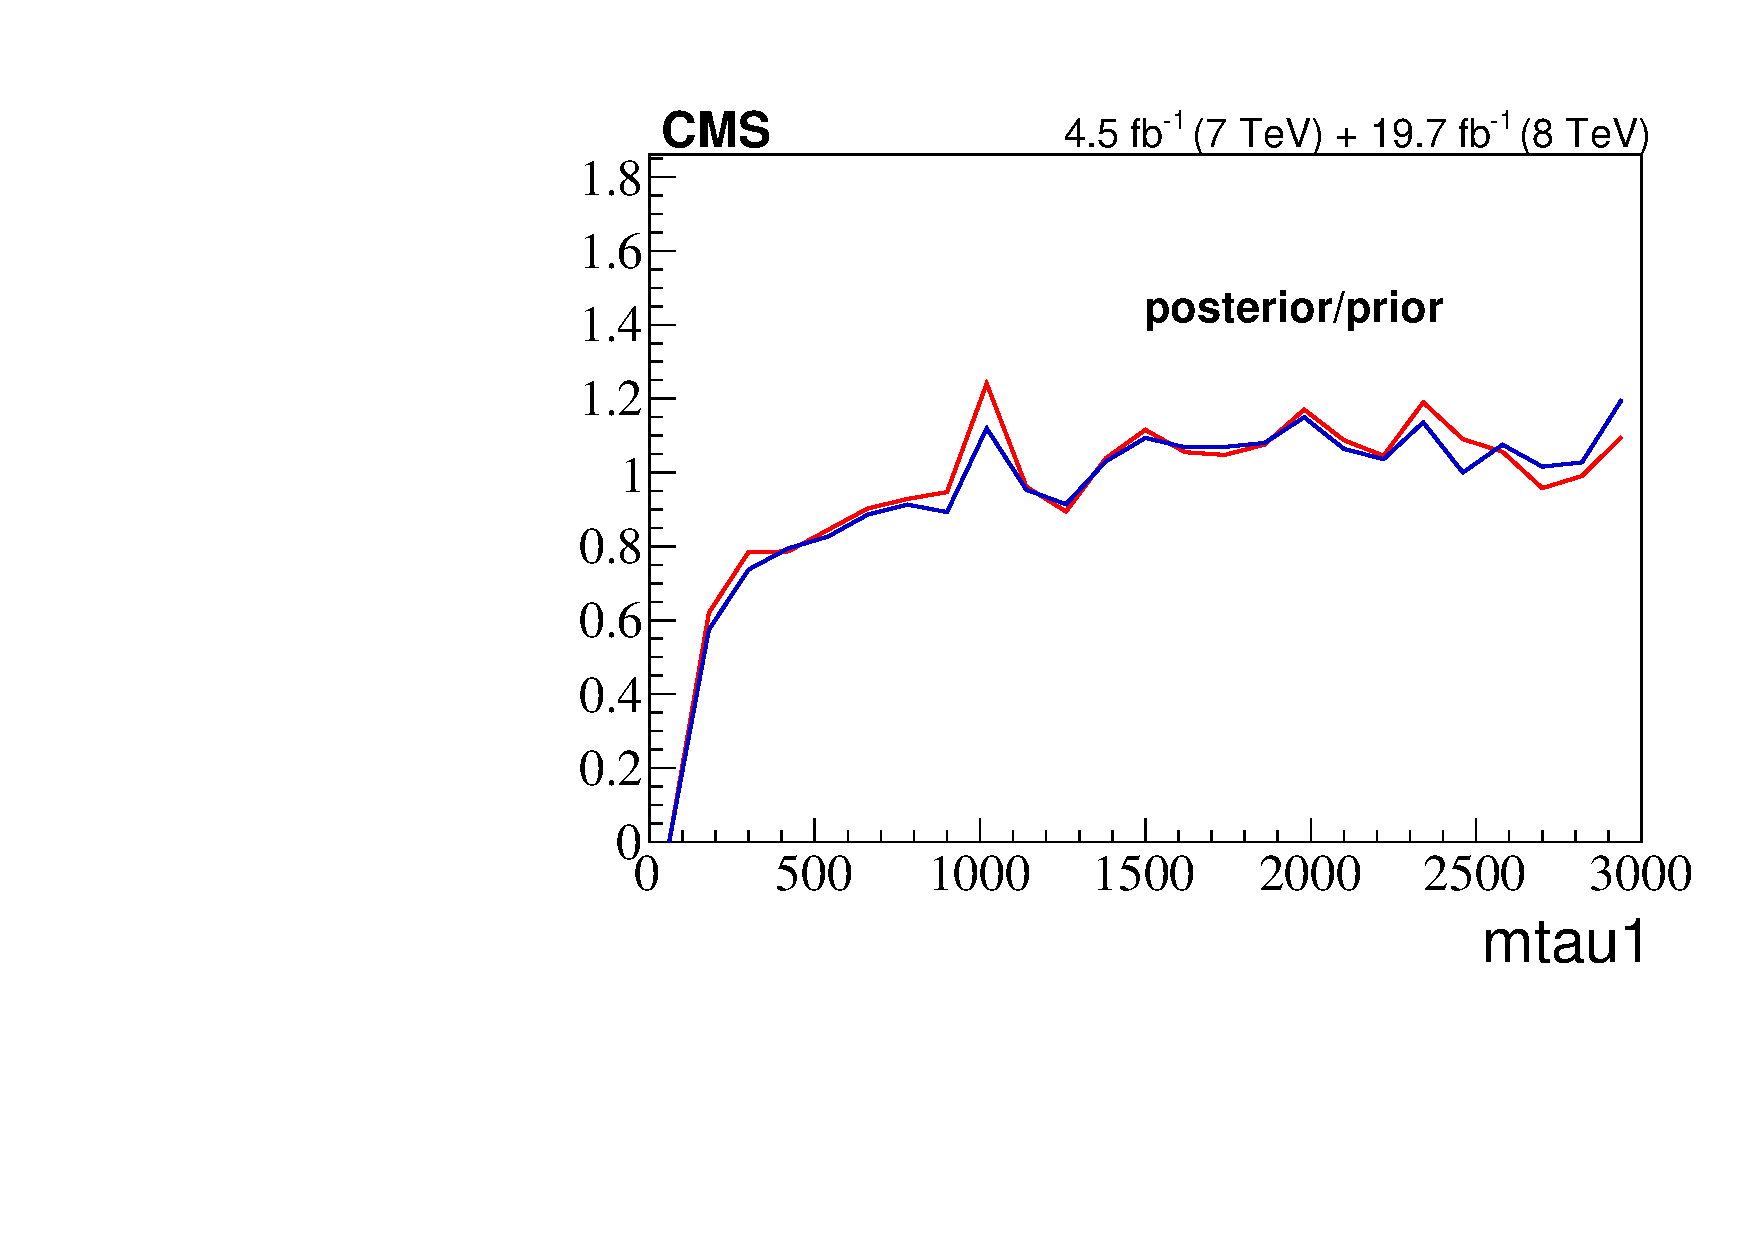
\includegraphics[width=0.5\linewidth]{figures/pMSSMpaper/Prior/mtau1ratio.pdf}

}
\caption{Left: posterior/prior of $m_{\tilde{\text{l}}_1}$ (top) and $m_{\tilde{\tau}_1}$ (bottom). Right: Ratio of the posterior to the prior of $m_{\tilde{\text{l}}_1}$ (top) and $m_{\tilde{\tau}_1}$ (bottom).}
\label{fig:mg_muL}
\end{figure}


\begin{figure}[h]
\centering
\subfloat[]{
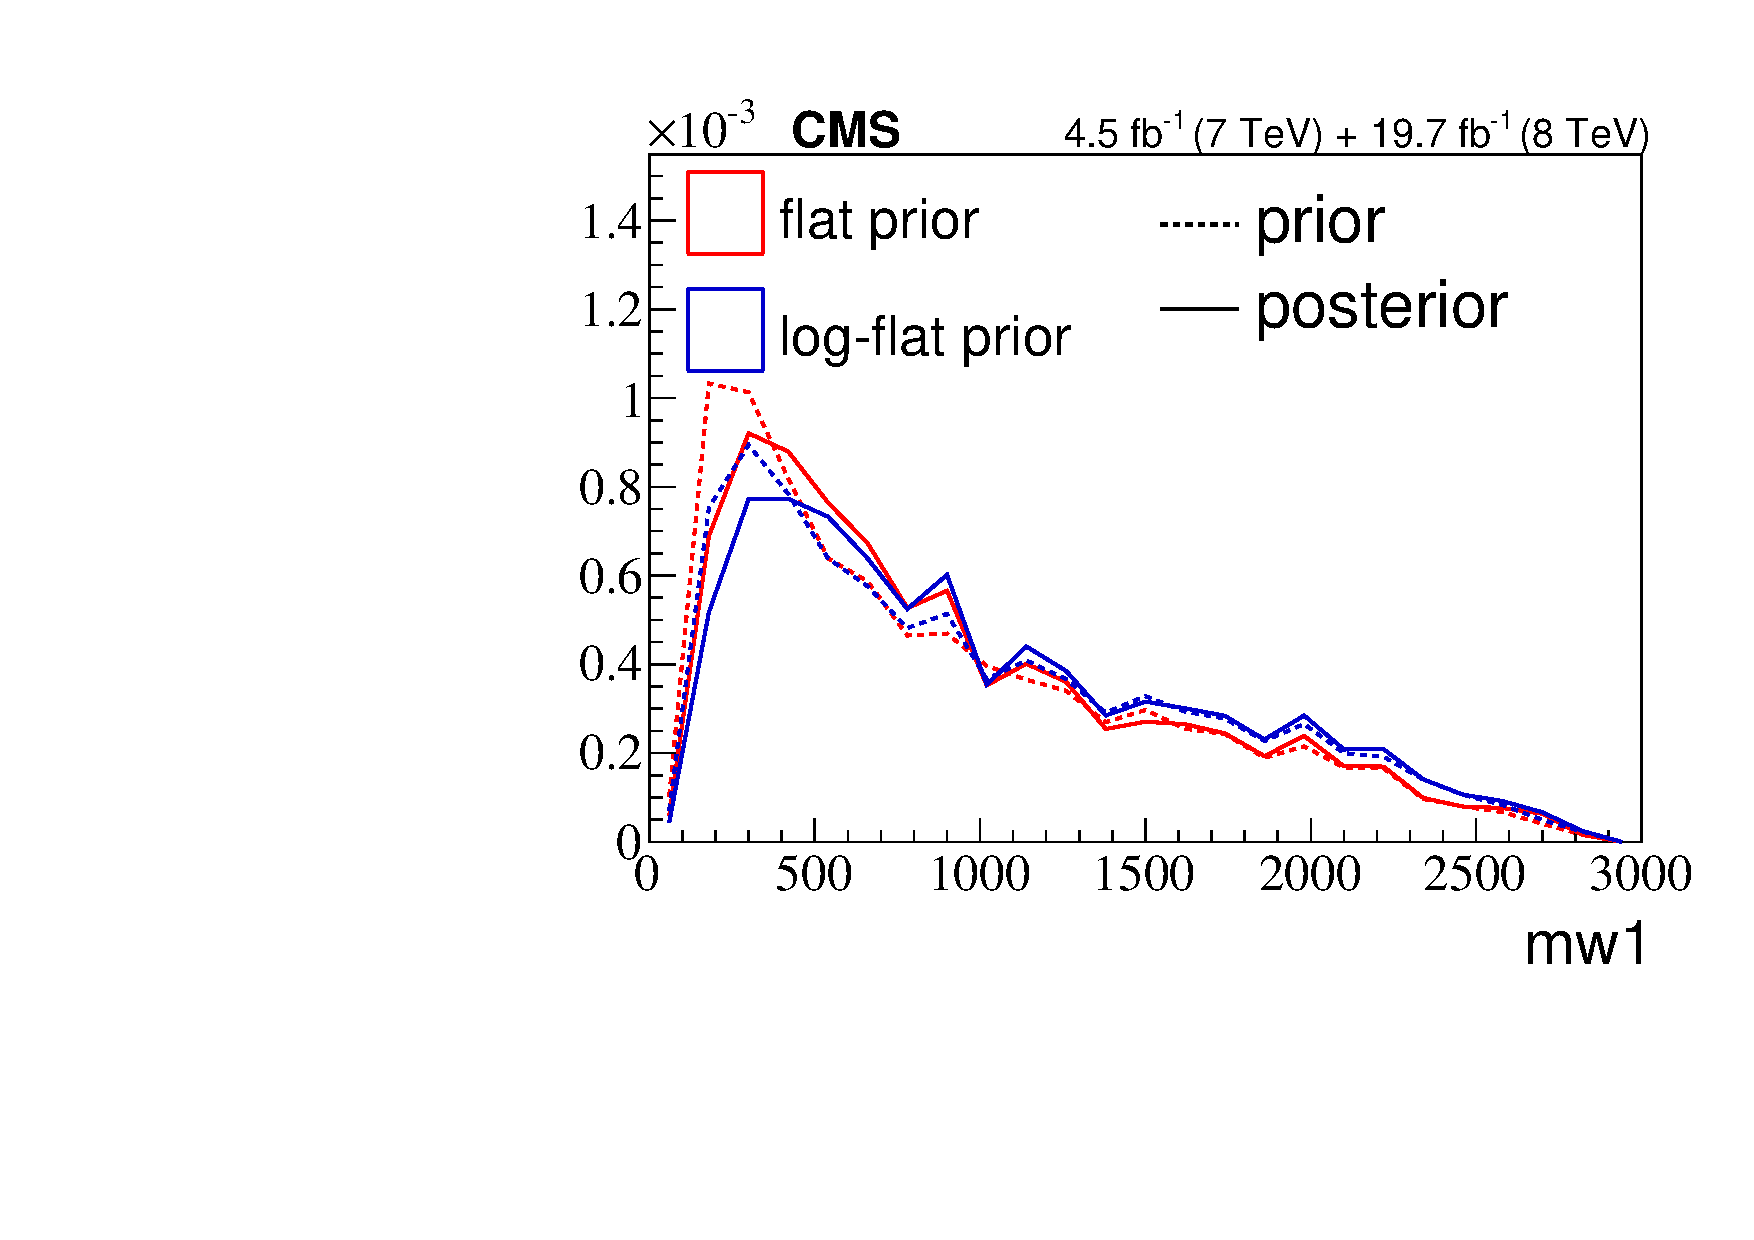
\includegraphics[width=0.5\linewidth]{figures/pMSSMpaper/Prior/mw1prepost.pdf}
}
\subfloat[]{
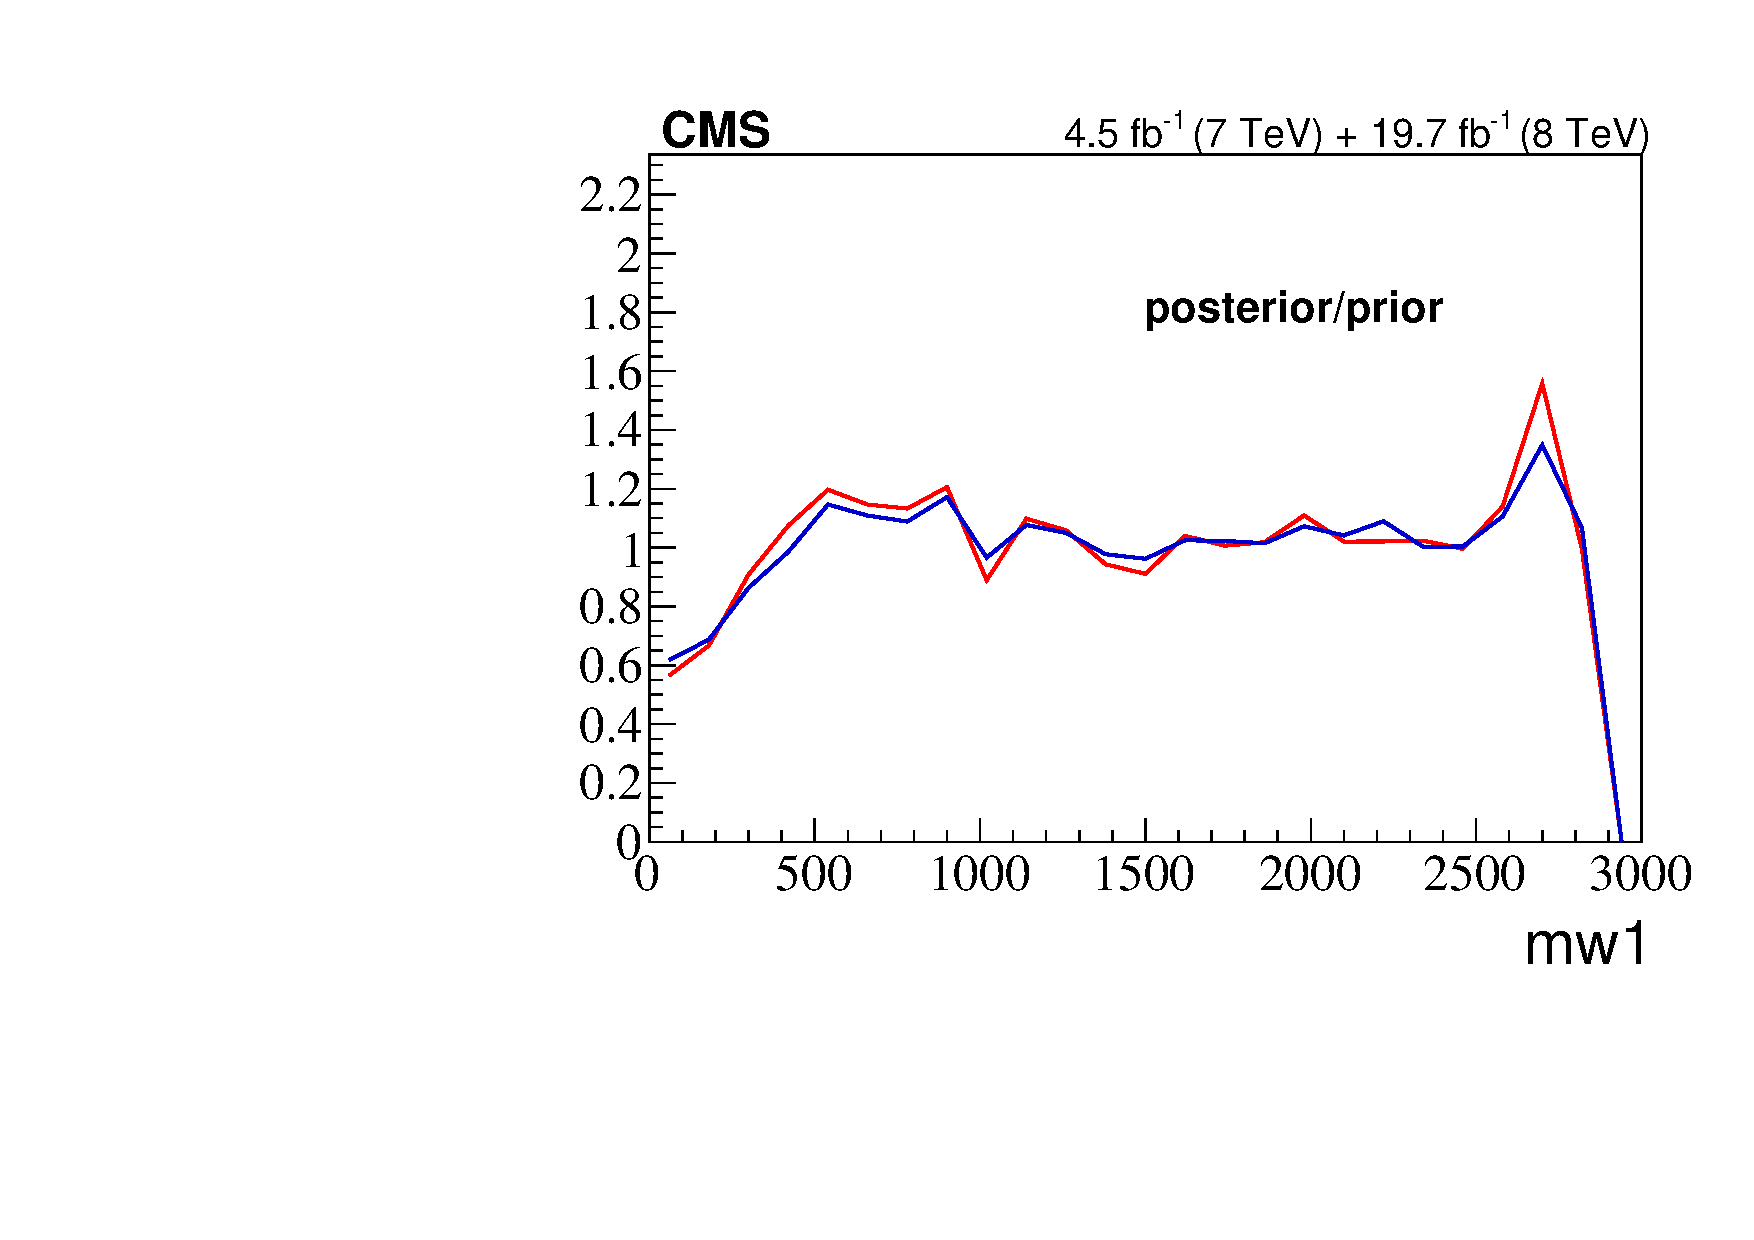
\includegraphics[width=0.5\linewidth]{figures/pMSSMpaper/Prior/mw1ratio.pdf}
}\\
\subfloat[]{
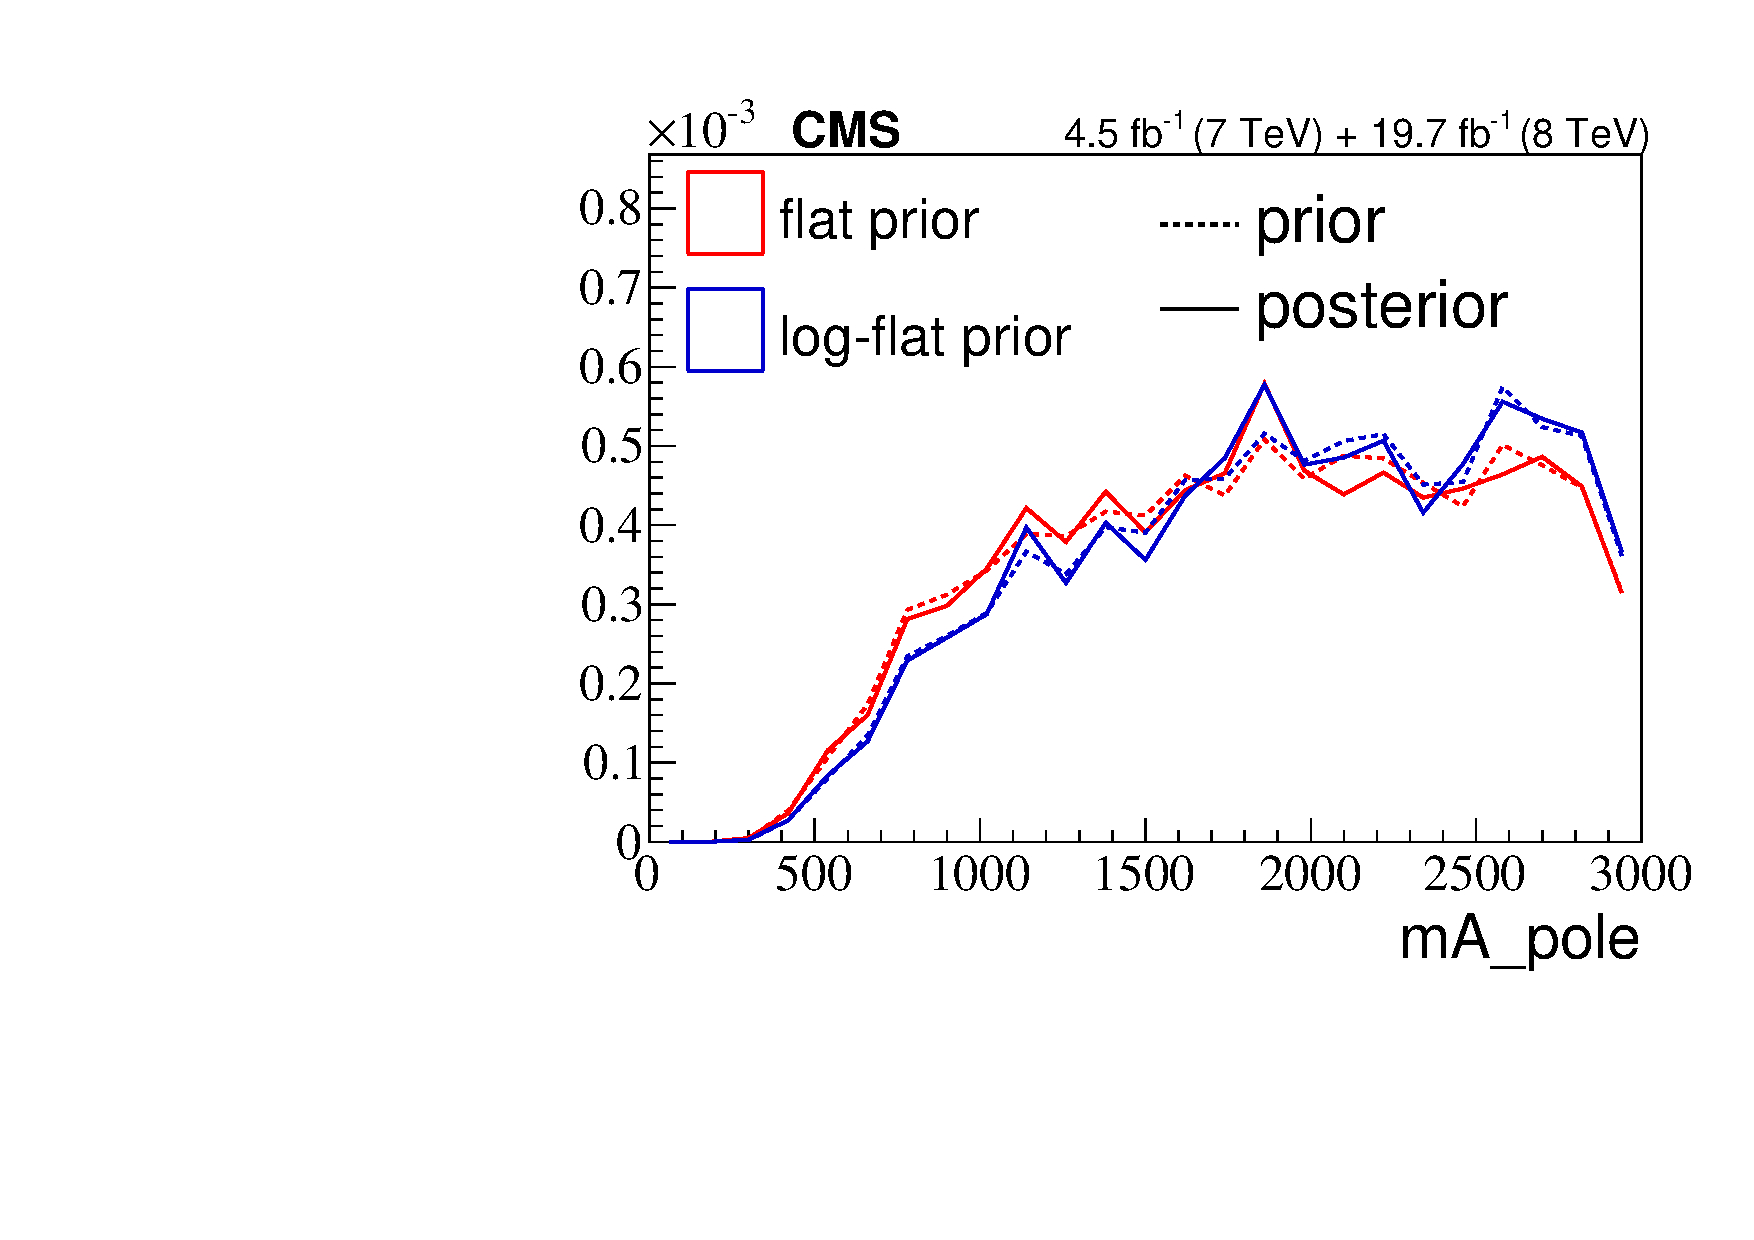
\includegraphics[width=0.5\linewidth]{figures/pMSSMpaper/Prior/mApoleprepost.pdf}
}
\subfloat[]{
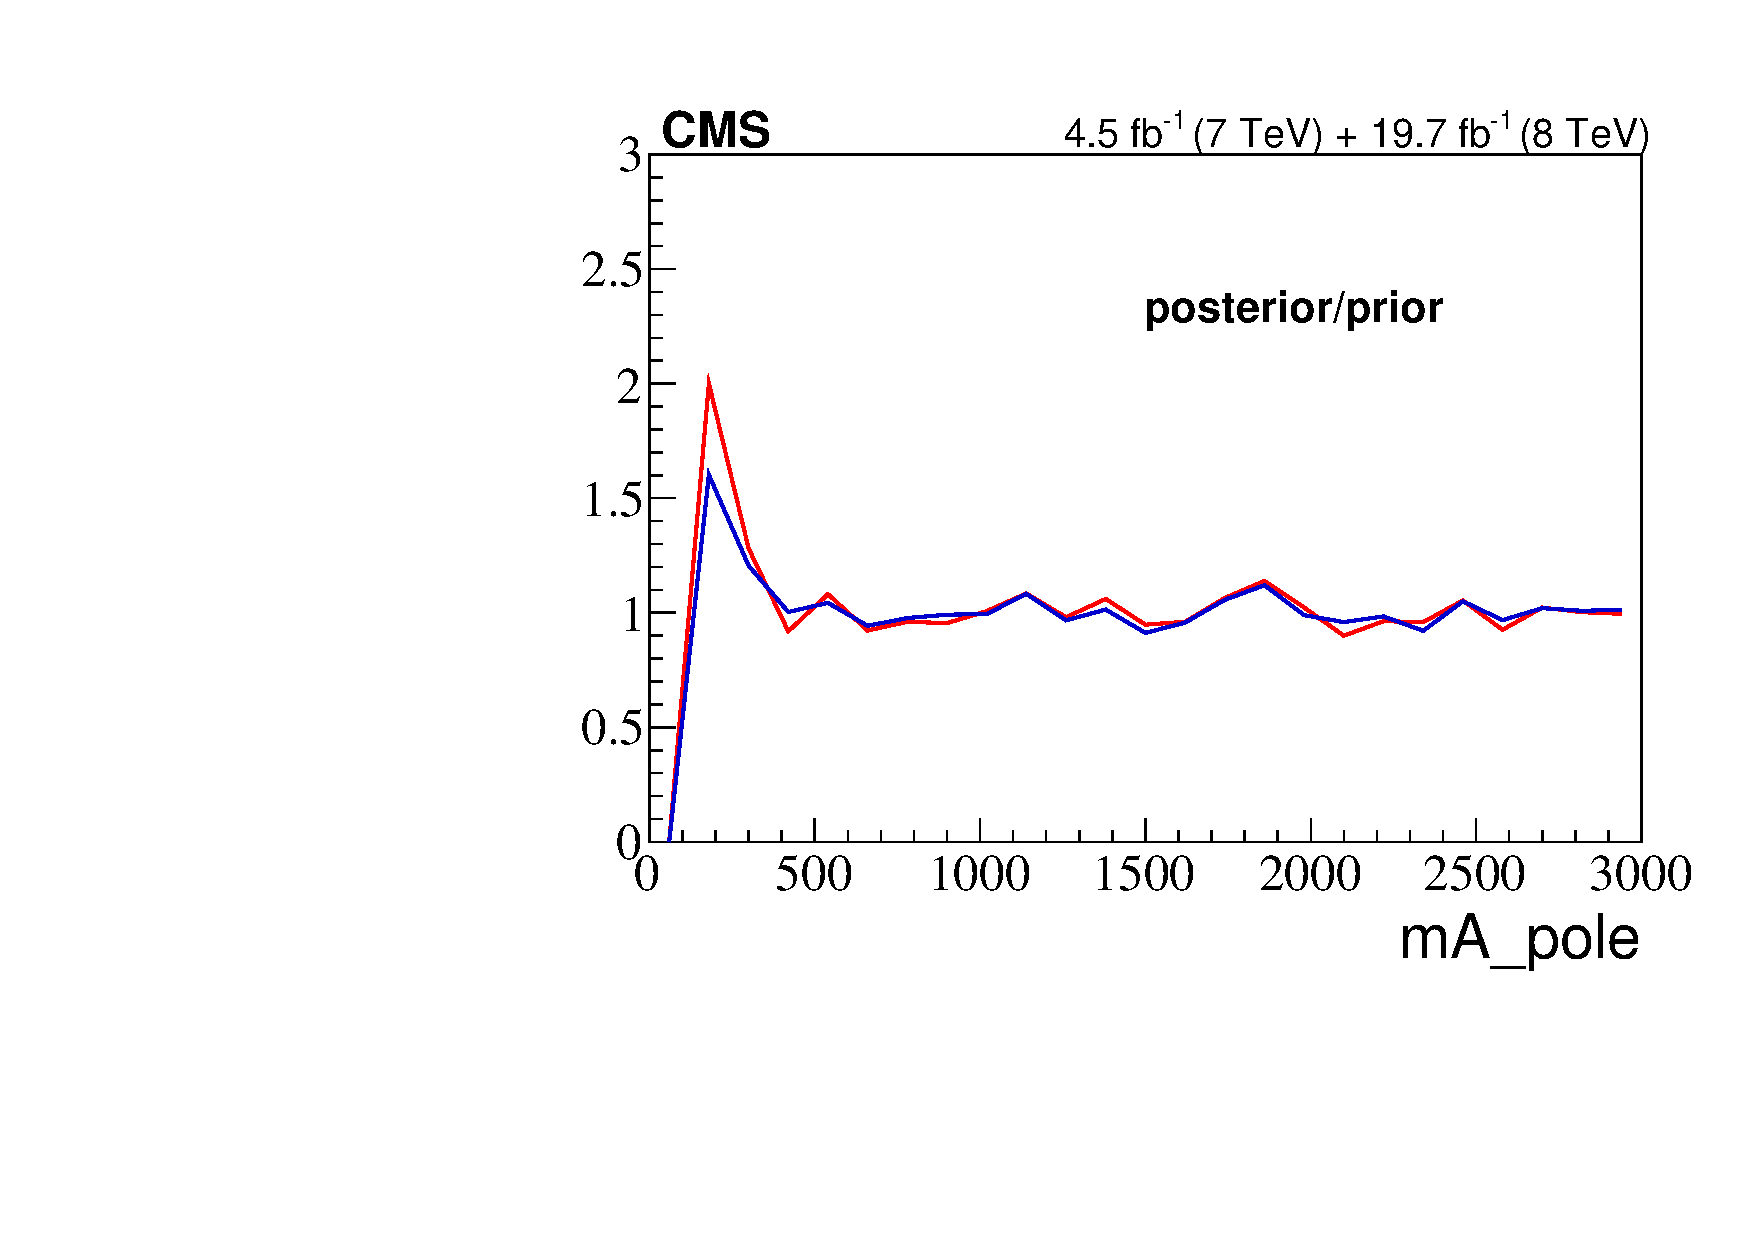
\includegraphics[width=0.5\linewidth]{figures/pMSSMpaper/Prior/mApoleratio.pdf}
}
\caption{Left: posterior/prior of $m_{\tilde{\chi}_{1}^{\pm}}$ (top) and $m_{A}$(pole) (bottom). Right: Ratio of the posterior to the prior of $m_{\tilde{\chi}_{1}^{\pm}}$ (top) and $m_{A}$(pole) (bottom).}
\label{fig:mg_muL}
\end{figure}
\FloatBarrier

\section{Profile vs marginal likelihoods}
\label{sec:freqcheck}
Experience suggests that when profile and marginal likelihoods are in approximate agreement, the conclusions obtained via frequentist and Bayesian methods approximately agree. Therefore, it is
instructive to examine the profile likelihoods. To do so, 
a smooth analytic expression for the 19-D non-DCS likelihood is constructed. The non-DCS likelihood can be factorized as a separable component equal to the product of 19 1-D functions, and a correction function that accounts for the statistical dependencies among parameters, which, for simplicity, are referred to using the slightly imprecise term ``correlation'':
\begin{equation}
P(D^{\rm non-DCS}|\vec{\theta}\ ) = {\rm C}(\vec{\theta}\ ) \cdot \prod_{i}^{19}f(\theta_{i}),
\label{eq:Likelihood}
\end{equation}
where $\vec{\theta}$ is a vector of the 19 pMSSM parameters of which $\theta_i$ is the $i$th element, the $f(\theta_{i})$ functions are the 1-D non-DCS marginal likelihoods,
\begin{equation}
f(\theta_i) = \int_1 d\theta_1 \cdots \int_j d\theta_j \cdots P(D^{\rm non-DCS}|\vec{\theta}\ ) \, \pi_F(\vec{\theta}\ ) \quad j \neq i,
\end{equation}
 using a flat ur-prior, $\pi_F(\vec{\theta}\ )$, and C($\vec{\theta}$\ ) encodes the correlations between the pMSSM parameters induced by the non-DCS measurements and constraints. 

The 1-D $f$ functions are estimated using TMVA regression methods~\cite{Hocker:2007ht}. For each regression, the swarm of points that constitute a discretized approximation to the non-DCS likelihood is projected onto a single pMSSM parameter, forming a 1-D histogram. The heights of the histogram bins are taken as the target, and the centers of the bins are taken as the input variable. A multi-layer perceptron (MLP)\cite{Hocker:2007ht} is trained on a portion of the pMSSM points.
The resulting $f(\theta_i) \equiv$ MLP($\theta_i$) functions are shown in Figures \ref{fig:KdeMlp}, along with the target histograms. The MLP approximations are seen to be reasonable.

The correlation function C($\theta$) is estimated using a multivariate classifier whose training sample consists of signal events corresponding to the original scan points, and background events consisting of pseudo-data generated from a sampling of the separable regression product. The classifier is an MLP whose output (see Figure \ref{fig:Classifier}) can be interpreted generally as
\begin{equation}
D = \frac{p(\vec{\theta} | {\rm s})}{p(\vec{\theta} | {\rm s})+p(\vec{\theta} | {\rm b})},
\label{eq:mlp}
\end{equation}
given that the training was performed with equal numbers of signal (s) and background (b) events. In this case, the output is
\begin{equation}
D = \frac{p(D^{\rm non-DCS}|\vec{\theta}\ )}{p(D^{\rm non-DCS}|\vec{\theta}\ )+ \prod_{i}^{19}f(\theta_{i})}.
\label{eq:MLP}
\end{equation}
Rearranging Equation(\ref{eq:MLP}) gives
\begin{equation}
P(D^{\rm non-DCS}|\vec{\theta}\ ) = \frac{D}{1-D}\prod_{i}^{19}f(\theta_{i}),
\label{eq:Like}
\end{equation}
and the correlation function (Equation(\ref{eq:Likelihood})) is identified as
\begin{equation}
{\rm C}(\vec{\theta}\ ) = \frac{D}{1-D}.
\end{equation}
The 1-D profile likelihoods were derived by maximizing Equation \ref{eq:Like} with respect to the $n-1=18$ parameters. 

Comparisons between the profile likelihoods and the 1-D non-DCS  marginal likelihoods are given in Figures \ref{fig:PandP1}-\ref{fig:PandP4}.  The comparison shows general agreement to within $\sim$10\%, with a couple of exceptions. The first notable difference is in the bino mass Lagrangian parameter $M_1$, where the profile likelihood is relatively enhanced at large absolute values of $M_1$. If the LSP is bino-like,  confidence levels (CLs) based on the posterior densities would tend to under-exclude LSP masses; however, no LSP mass is excluded by the Z-significance, and so this does not alter the statement about LSPs made in the paper \ref{bib:pMSSM}. Finally, the trilinear coupling $A_t$ appears to have a roughly 30\% enhancement in the negative region for the likelihood with respect to the marginal likelihood. However, the paper makes no explicit statement about the impact of CMS analysis on the trilinear couplings. The otherwise general similarity of the two sets suggests that a frequentist analysis based on the profile likelihoods would yield conclusions consistent with those in the CMS pMSSM paper.  The Z-significance is a mapping of the Bayes factor that roughly maps to a frequentist n-sigma, the only difference being that rather than maximizing the likelihood to eliminate nuisance parameters, the likelihood is marginalized. 

\renewcommand*\thesubfigure{\arabic{subfigure}}
\begin{figure}[htbp]
\centering
\hspace{-8mm}
\subfloat[]{
  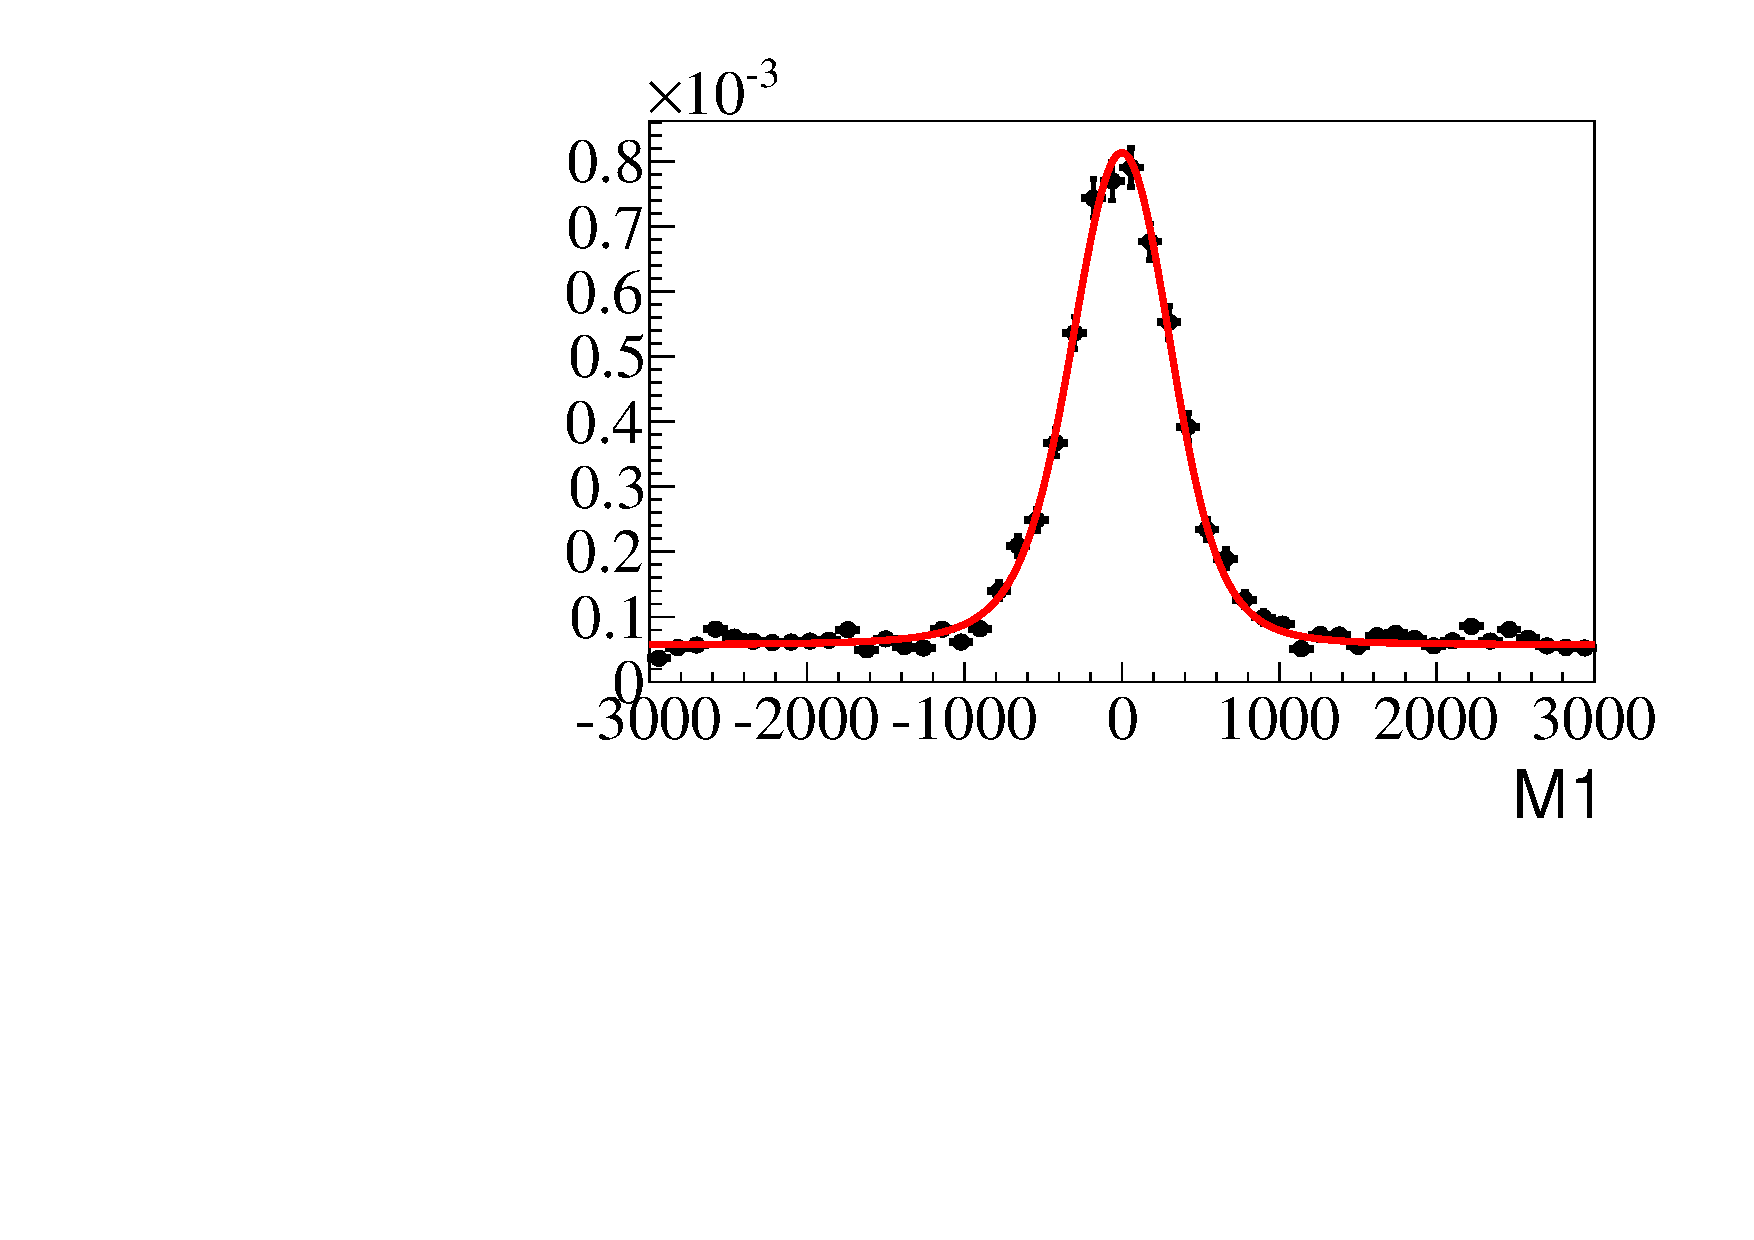
\includegraphics[width=50mm]{figures/pMSSMpaper/Prior/MLP/trainedRegression1_M1}
}
\hspace{-8mm}
\subfloat[]{
  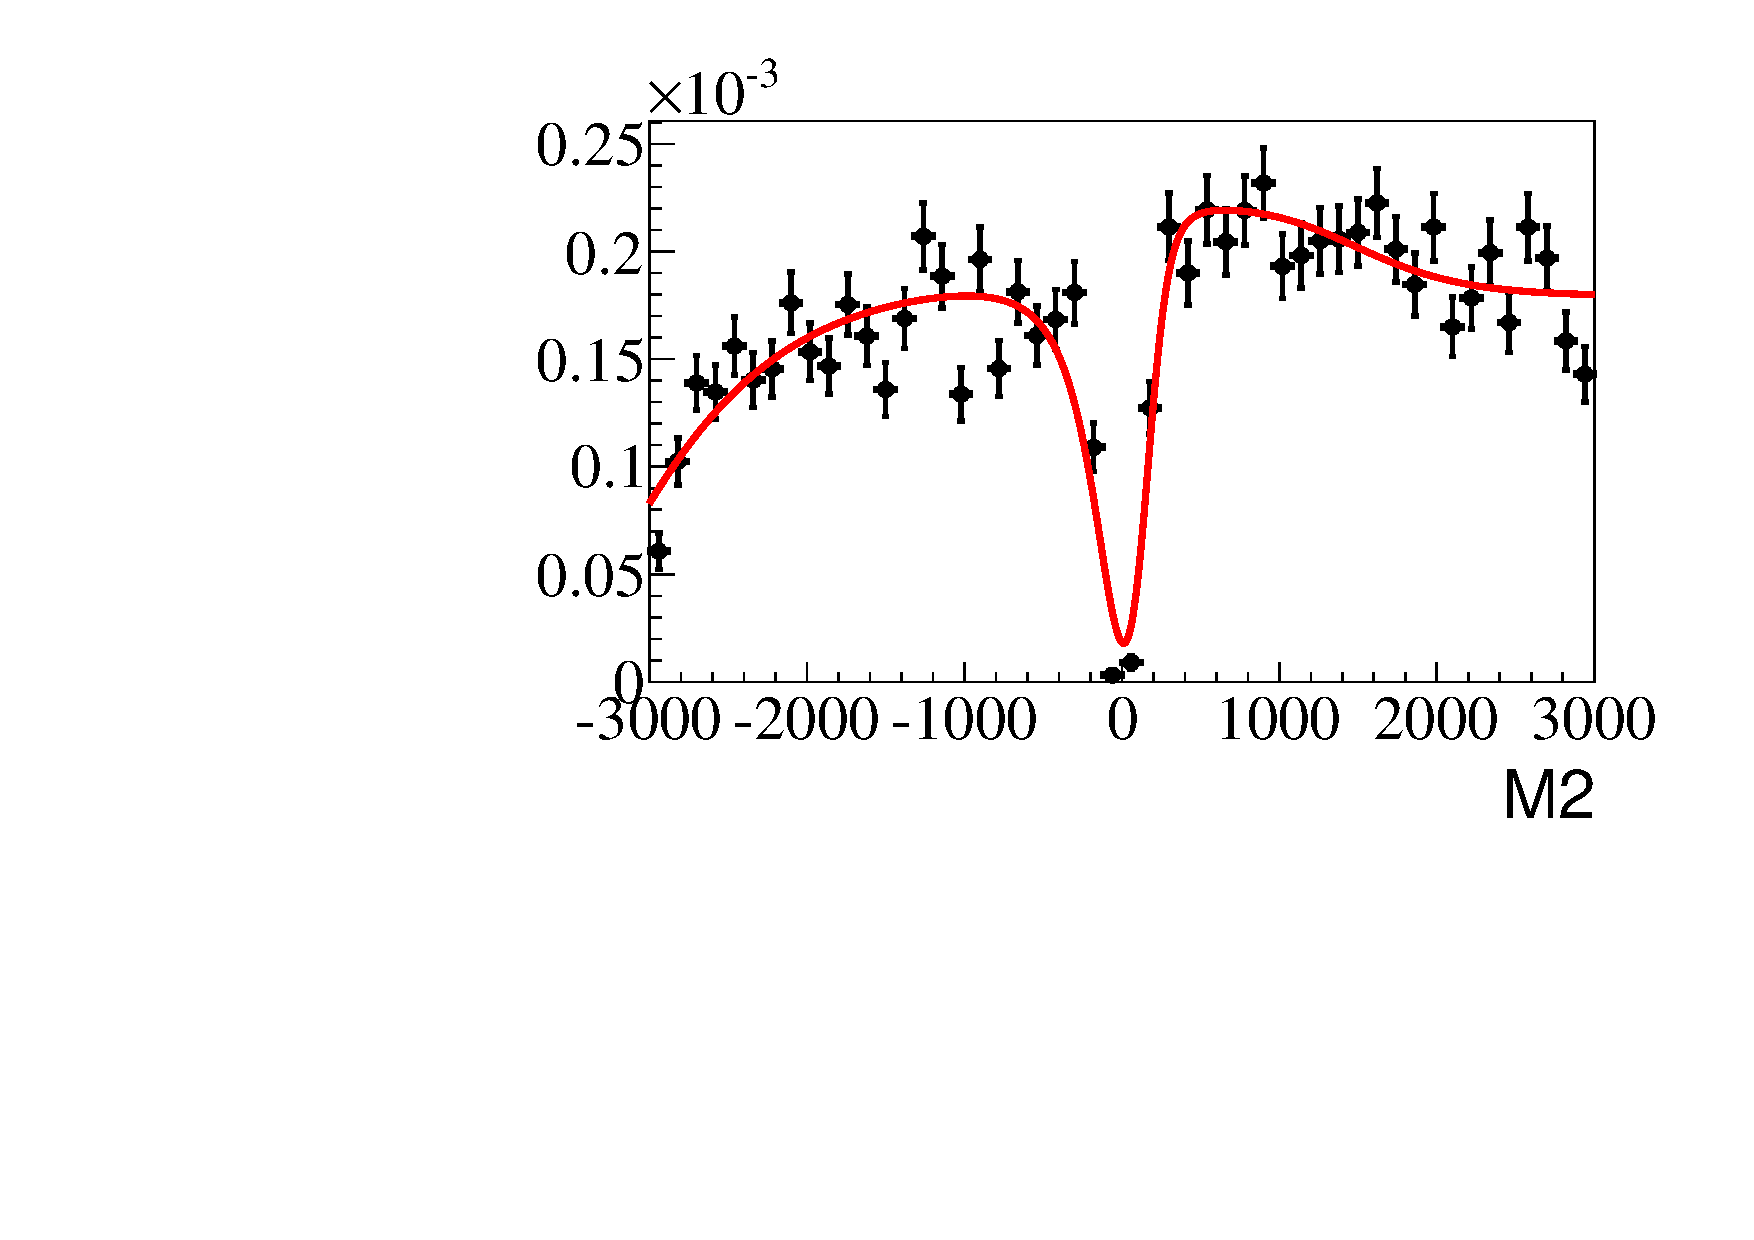
\includegraphics[width=50mm]{figures/pMSSMpaper/Prior/MLP/trainedRegression1_M2}
}
\hspace{-8mm}
\subfloat[]{
  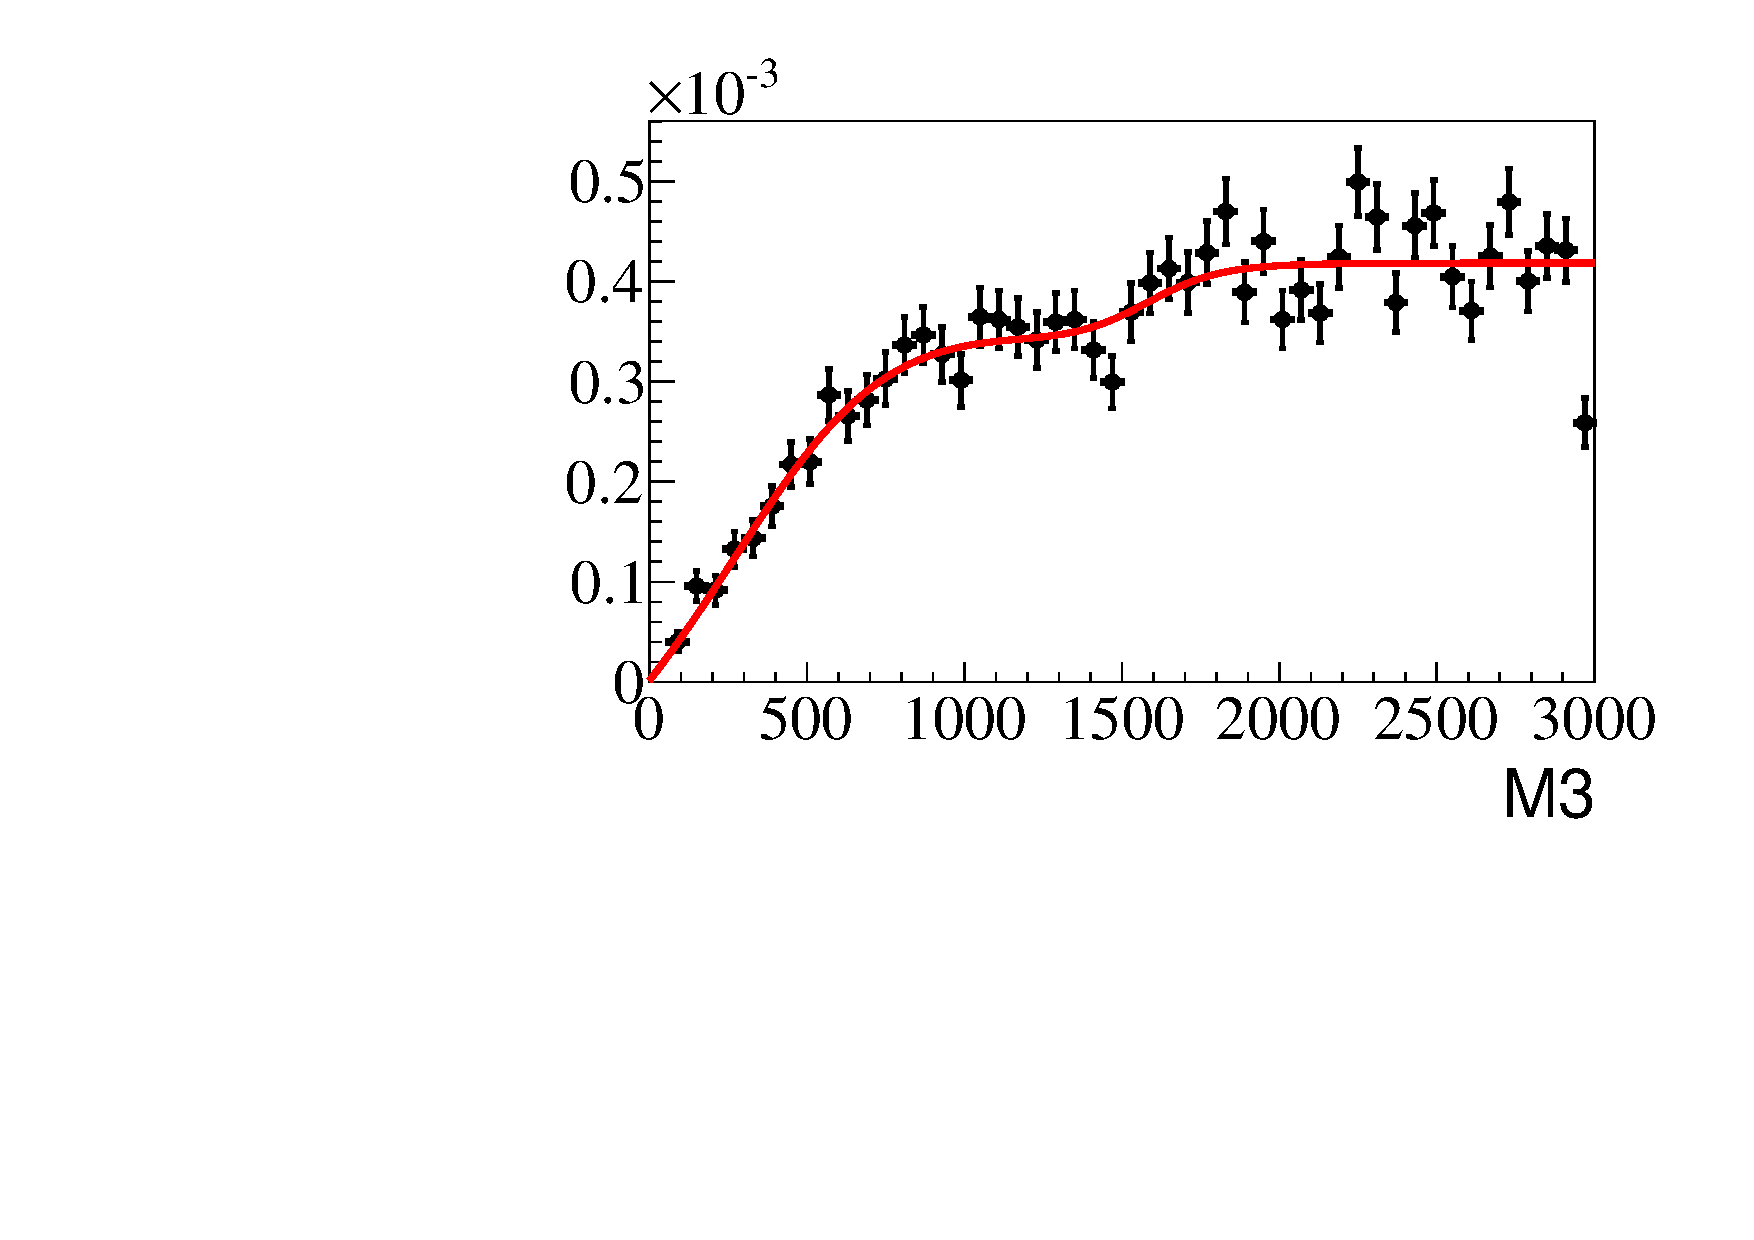
\includegraphics[width=50mm]{figures/pMSSMpaper/Prior/MLP/trainedRegression1_M3}
}
\hspace{-8mm}
\subfloat[]{
  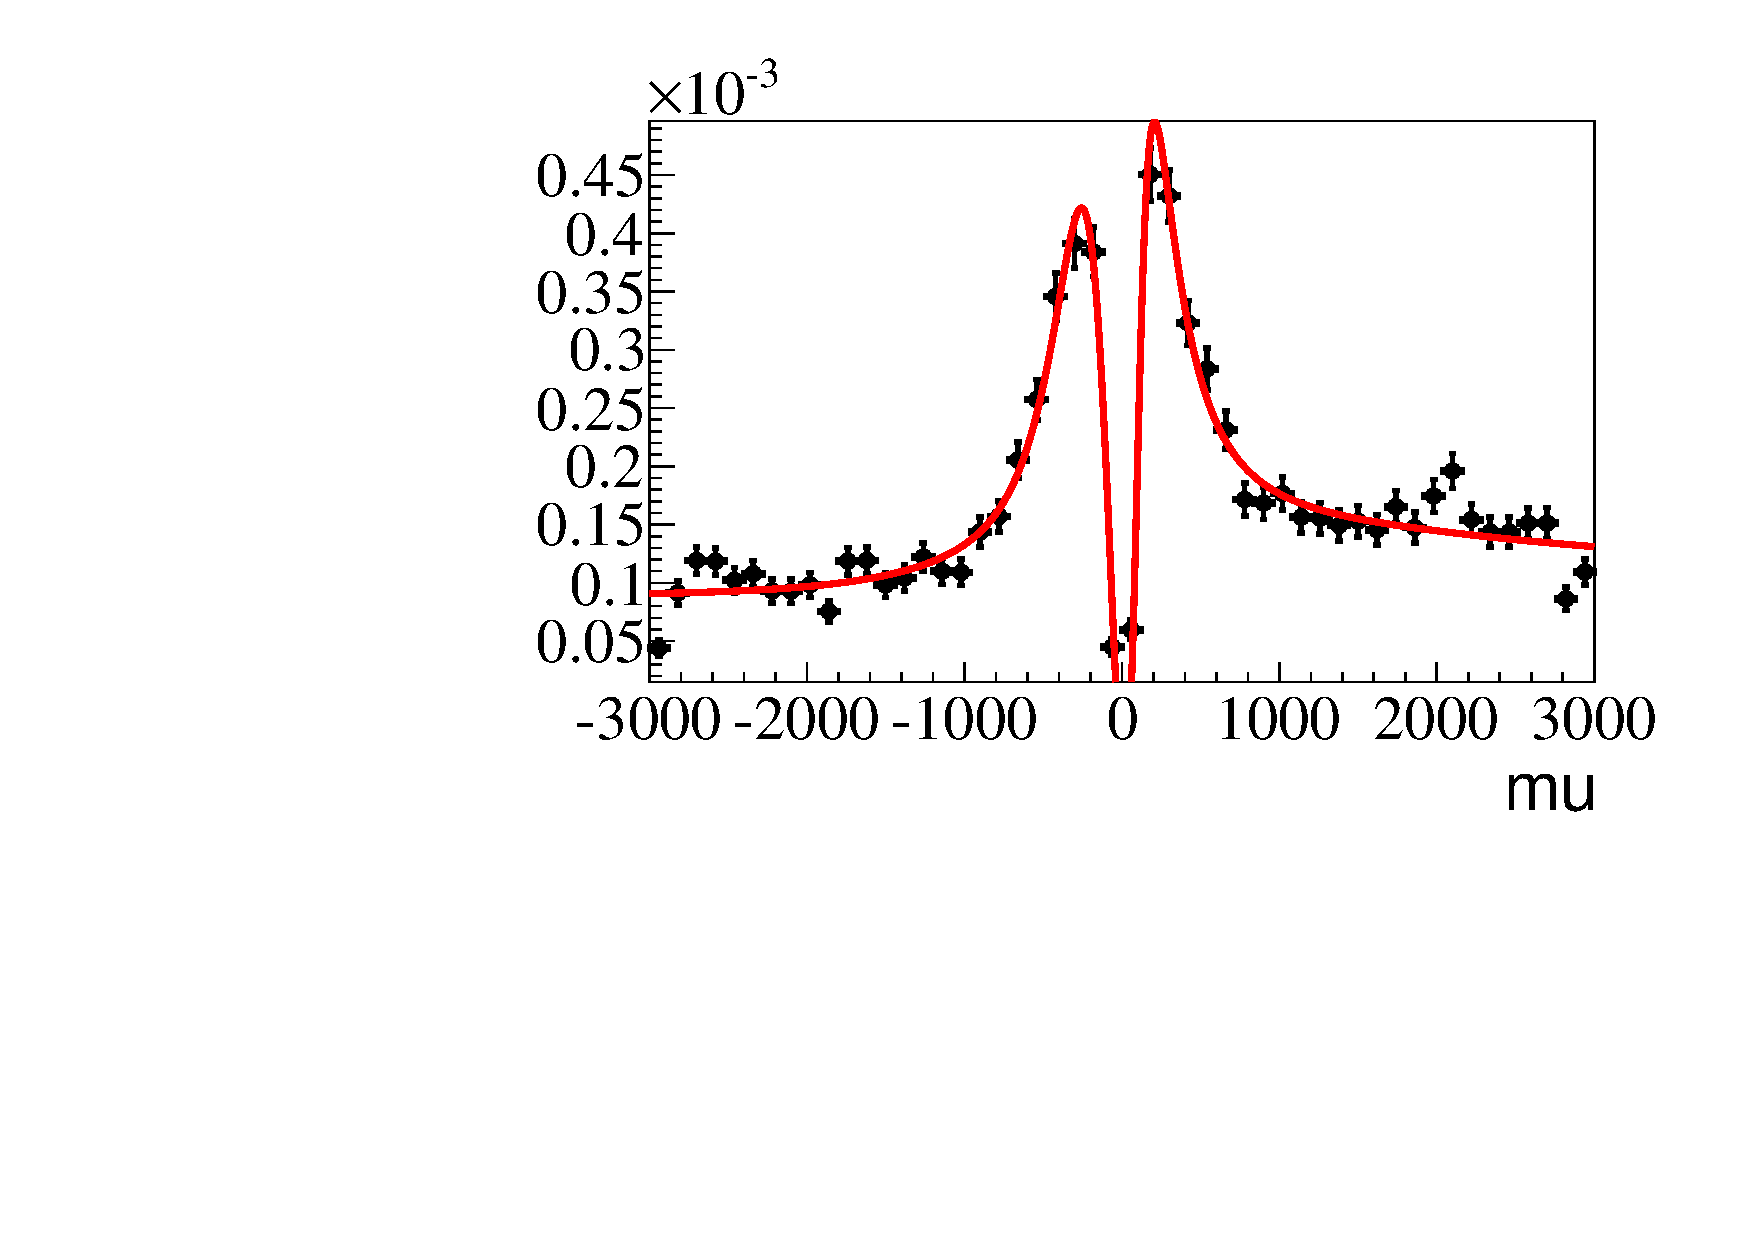
\includegraphics[width=50mm]{figures/pMSSMpaper/Prior/MLP/trainedRegression1_mu}
}
\hspace{-8mm}
\subfloat[]{   % ???
  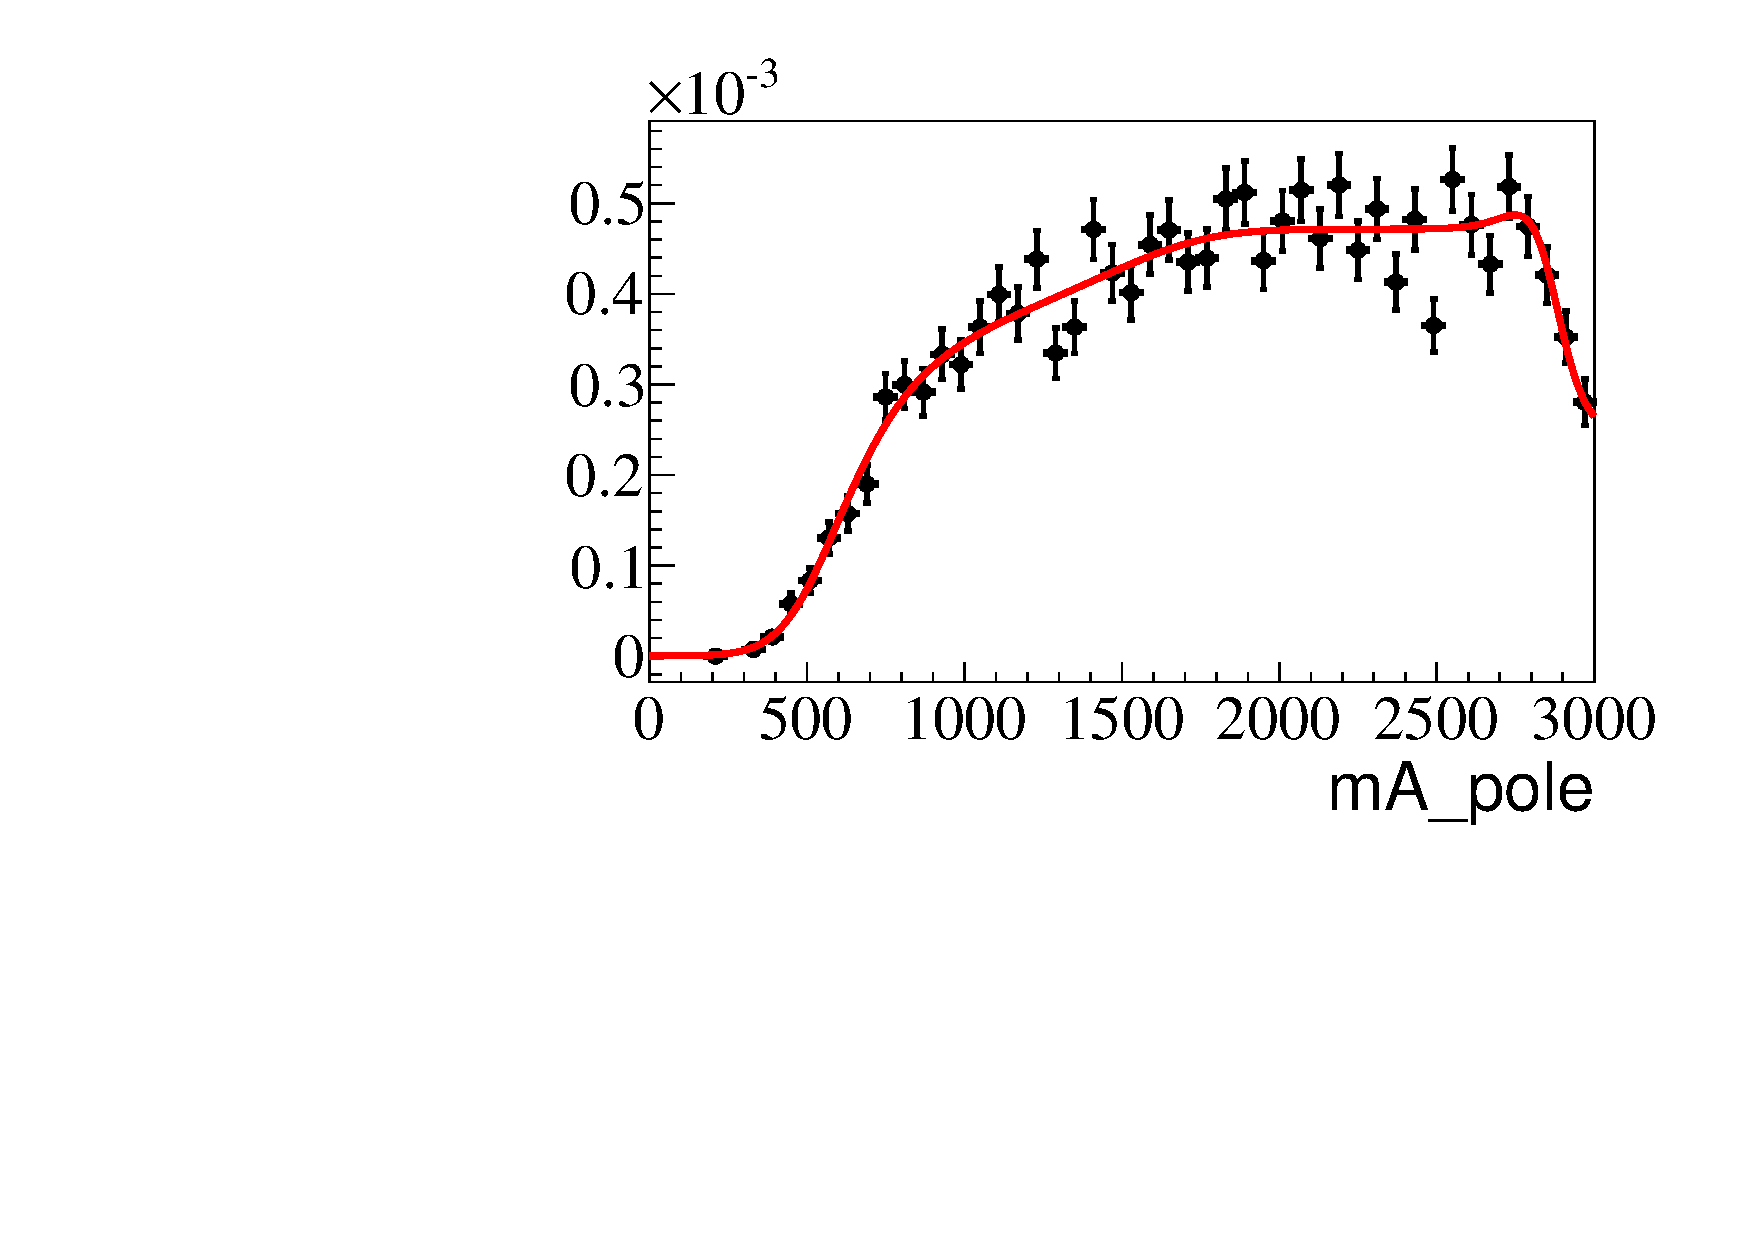
\includegraphics[width=50mm]{figures/pMSSMpaper/Prior/MLP/trainedRegression1_mA_pole}
}
\hspace{-8mm}
\subfloat[]{
  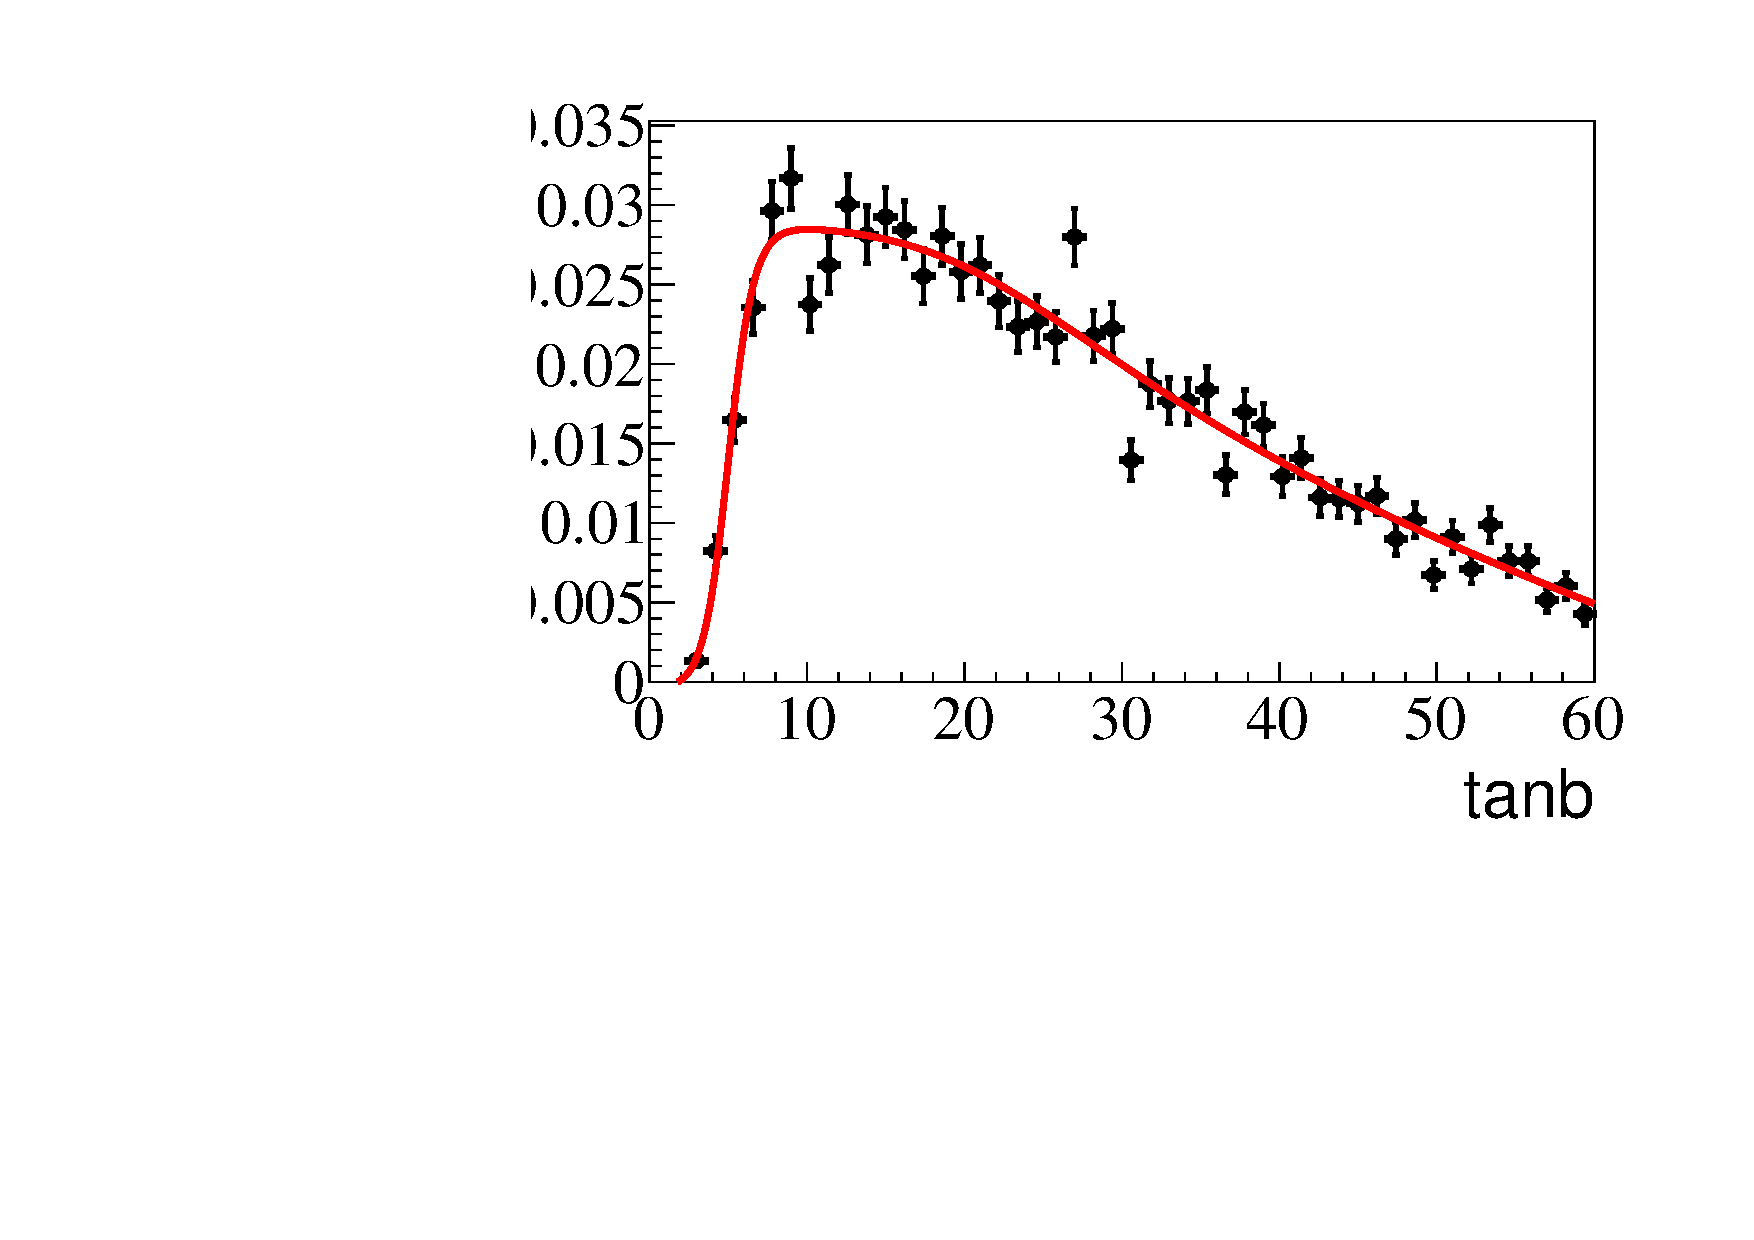
\includegraphics[width=50mm]{figures/pMSSMpaper/Prior/MLP/trainedRegression1_tanb}
}
\hspace{-8mm}
\subfloat[]{
  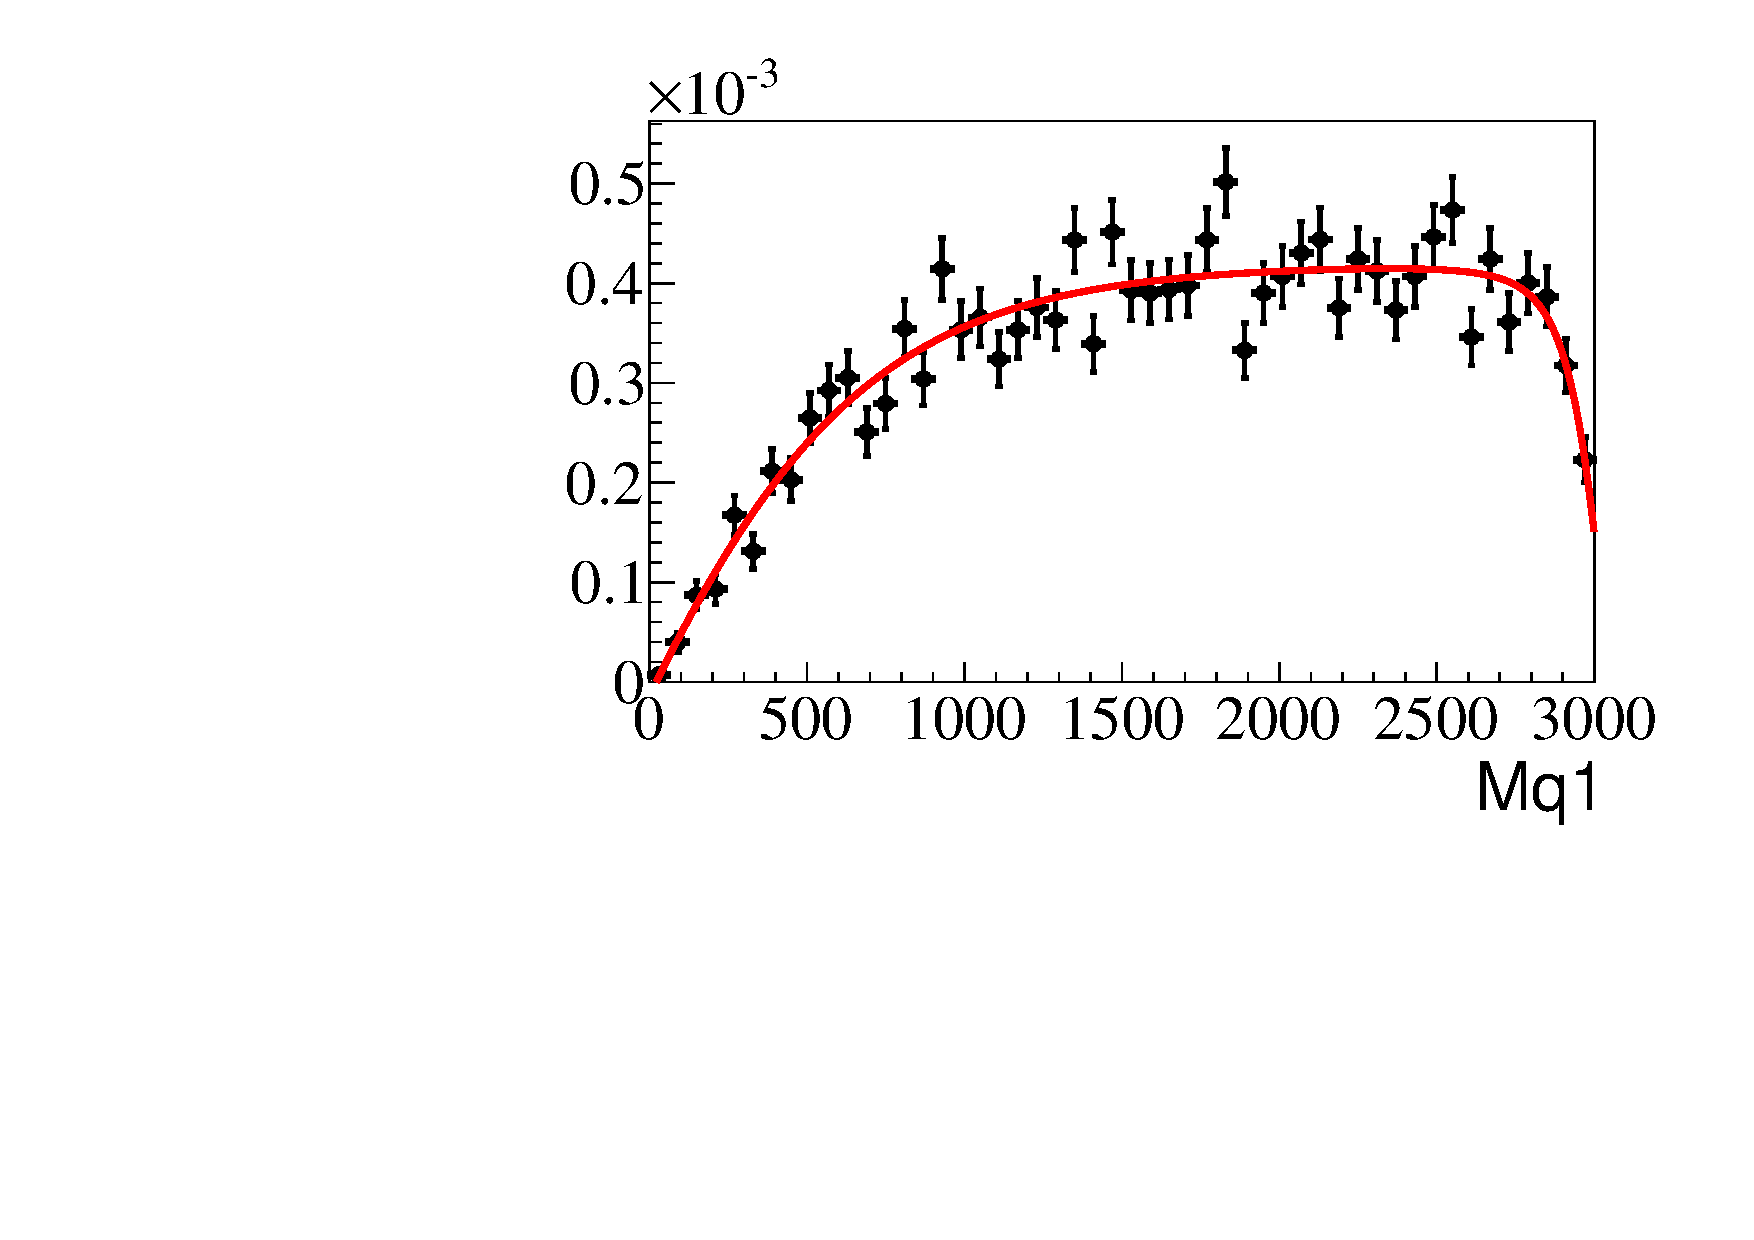
\includegraphics[width=50mm]{figures/pMSSMpaper/Prior/MLP/trainedRegression1_Mq1}
}
\hspace{-8mm}
\subfloat[]{
  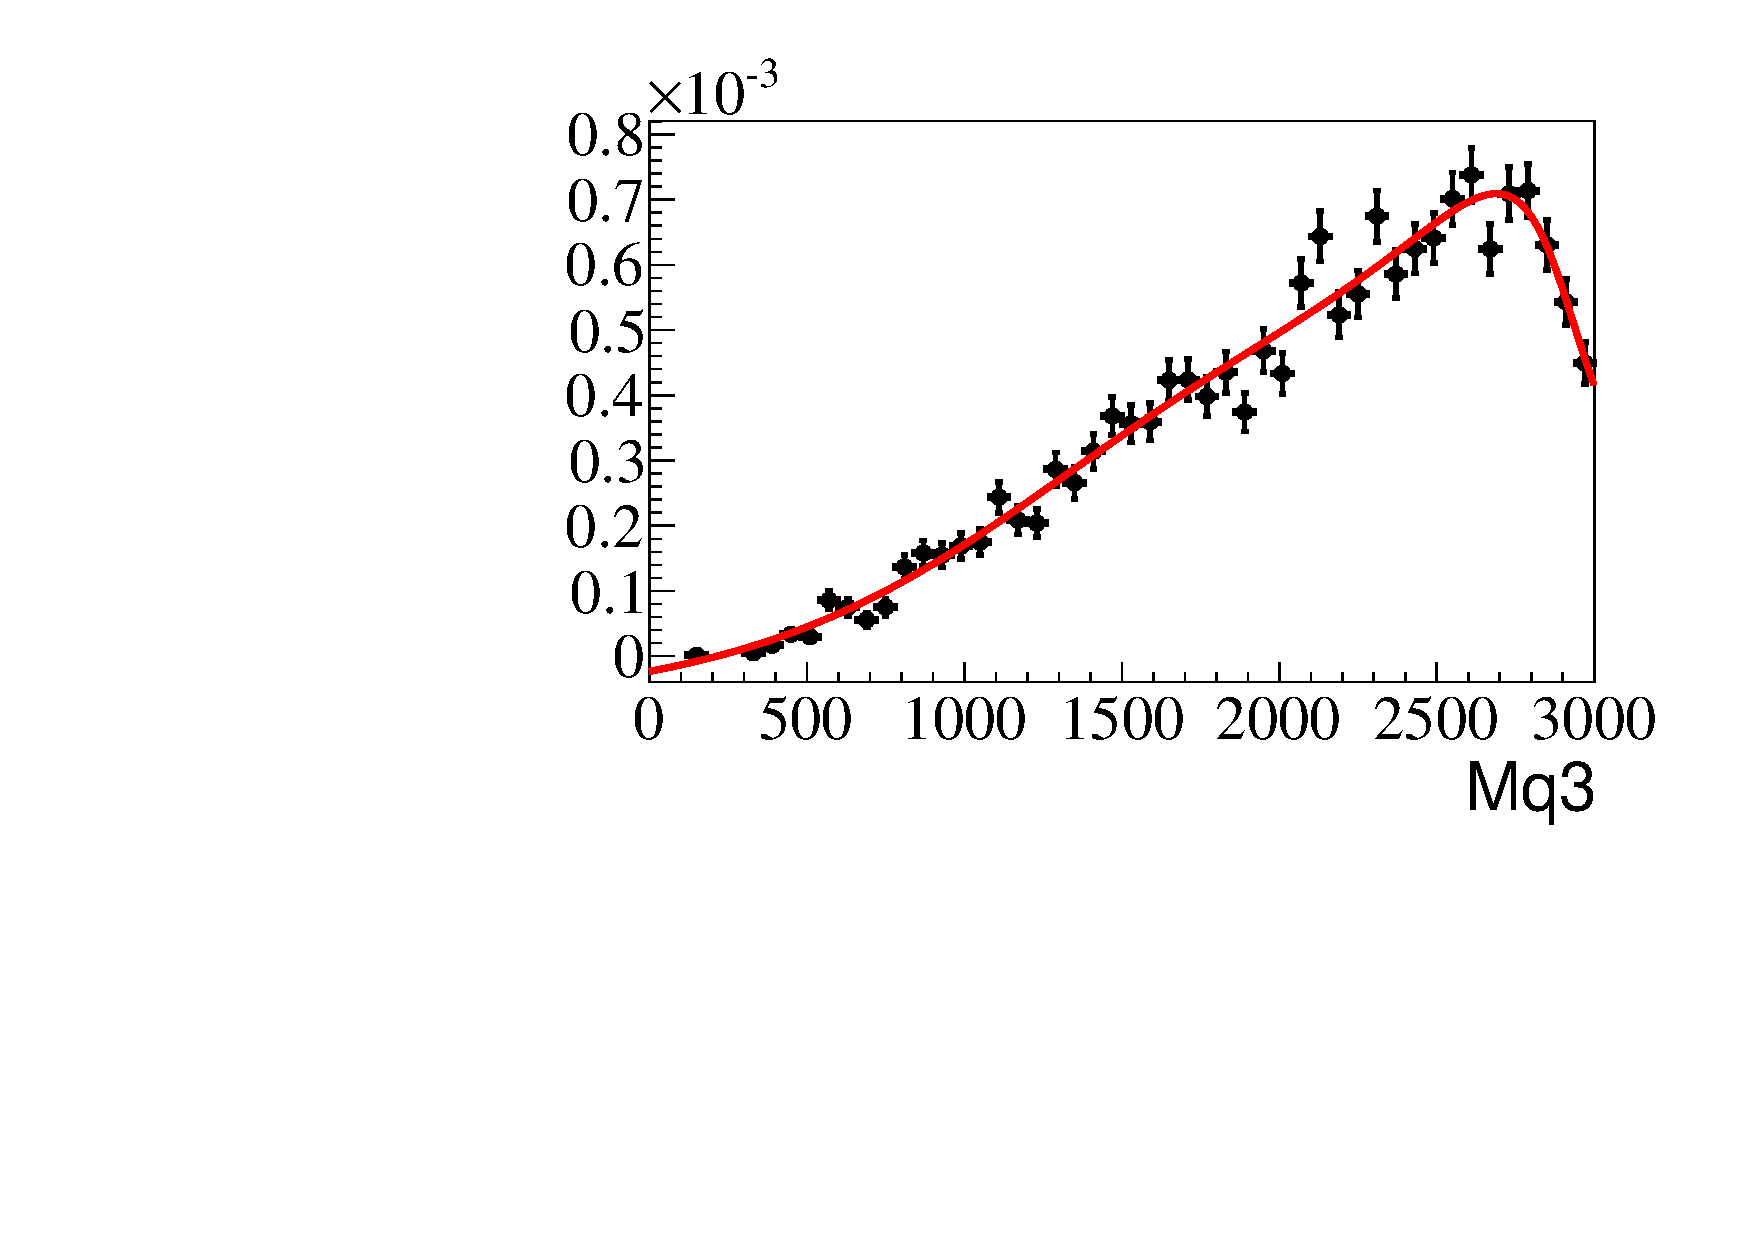
\includegraphics[width=50mm]{figures/pMSSMpaper/Prior/MLP/trainedRegression1_Mq3}
}
\hspace{-8mm}
\subfloat[]{
  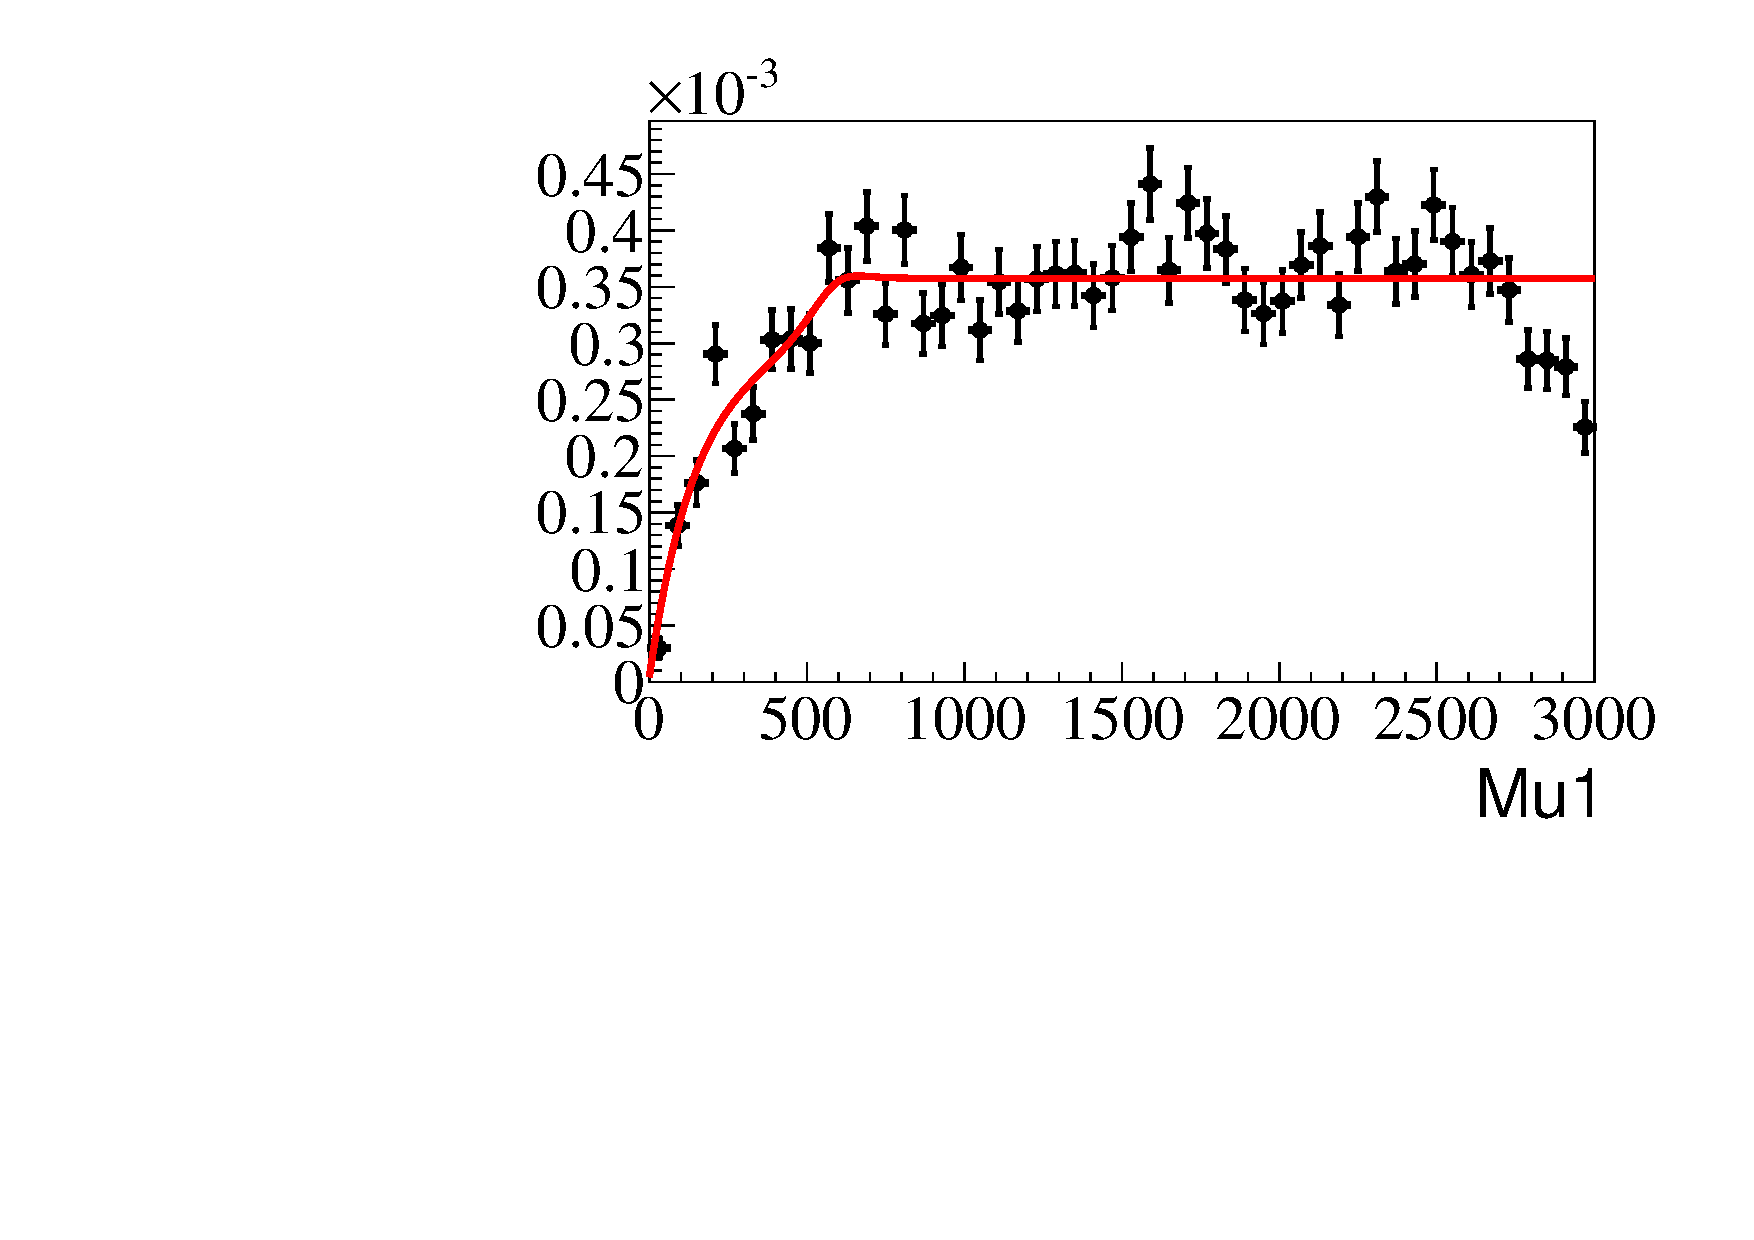
\includegraphics[width=50mm]{figures/pMSSMpaper/Prior/MLP/trainedRegression1_Mu1}
}
\hspace{-8mm}
\subfloat[]{
  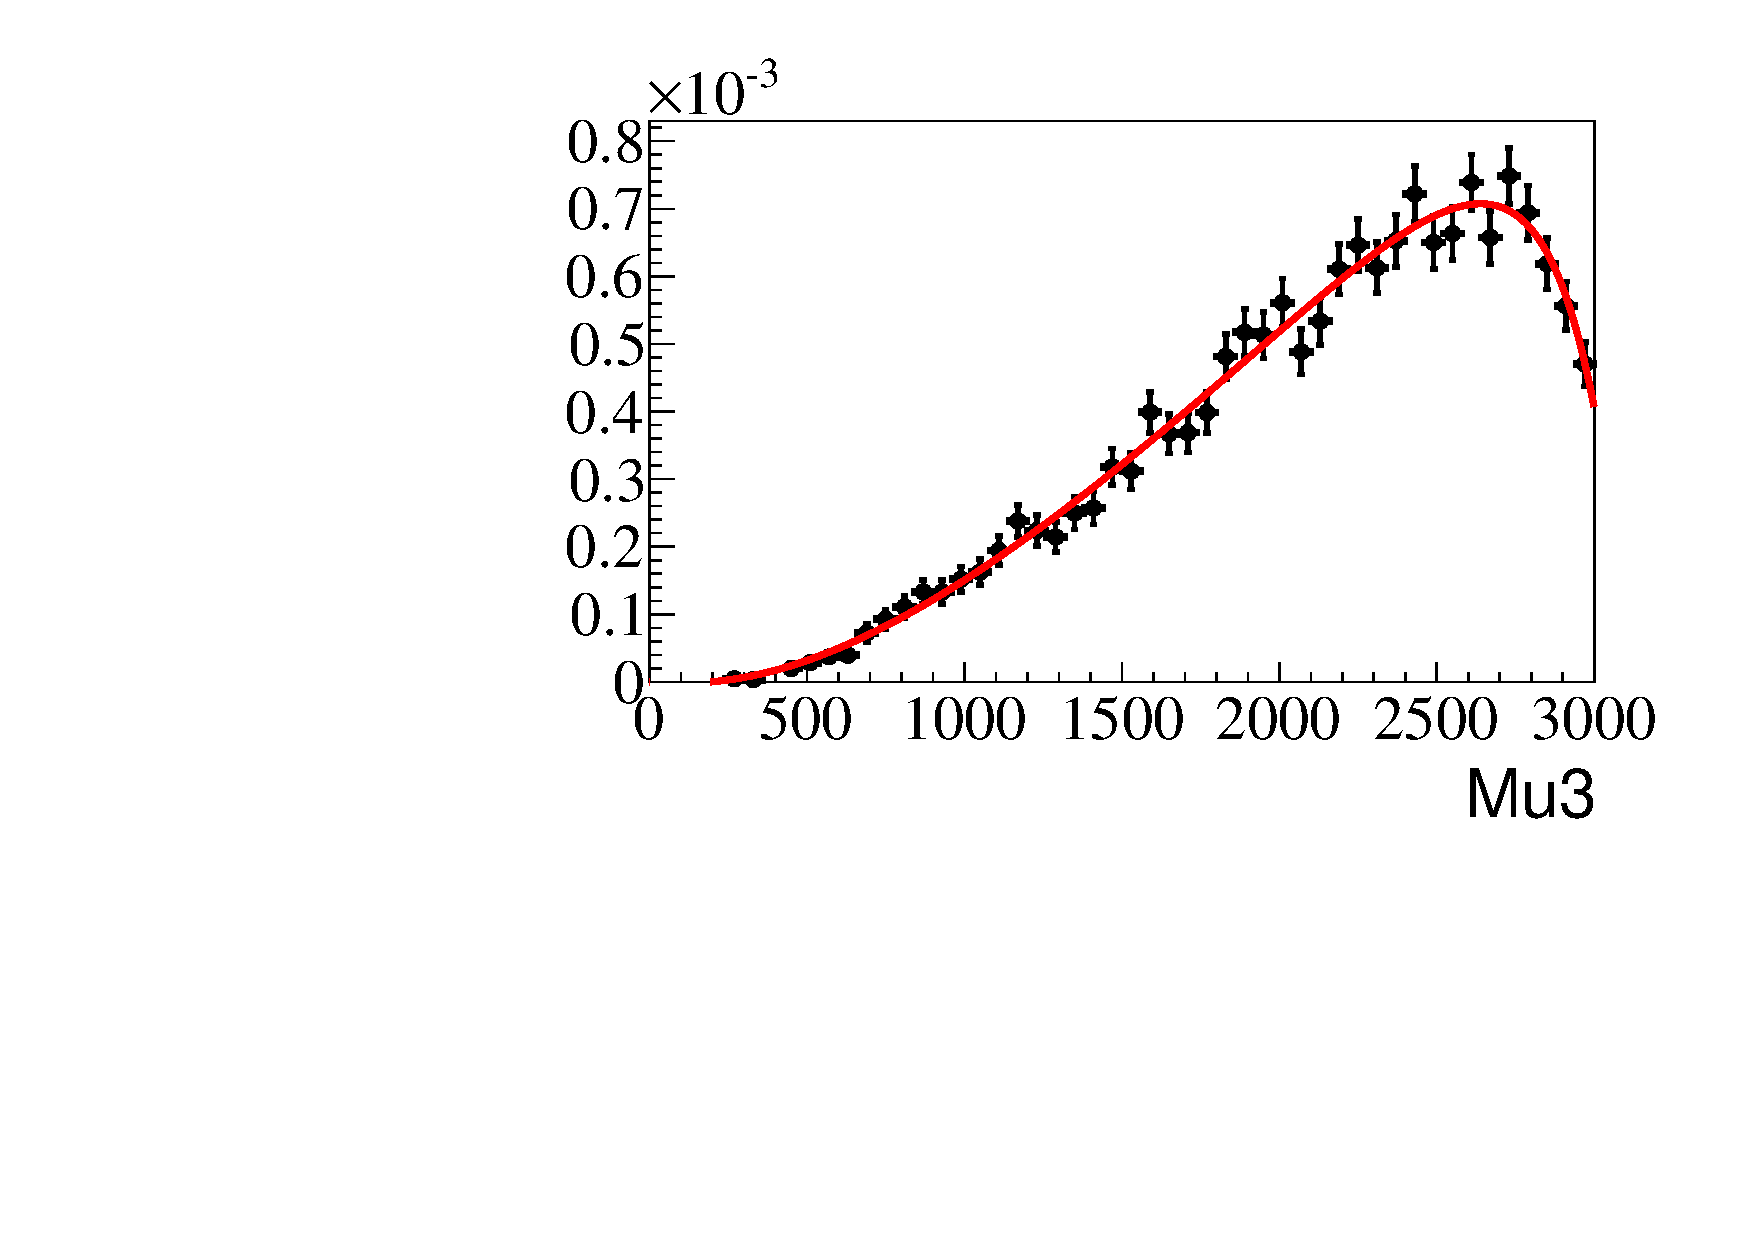
\includegraphics[width=50mm]{figures/pMSSMpaper/Prior/MLP/trainedRegression1_Mu3}
}
\hspace{-8mm}
\subfloat[]{
  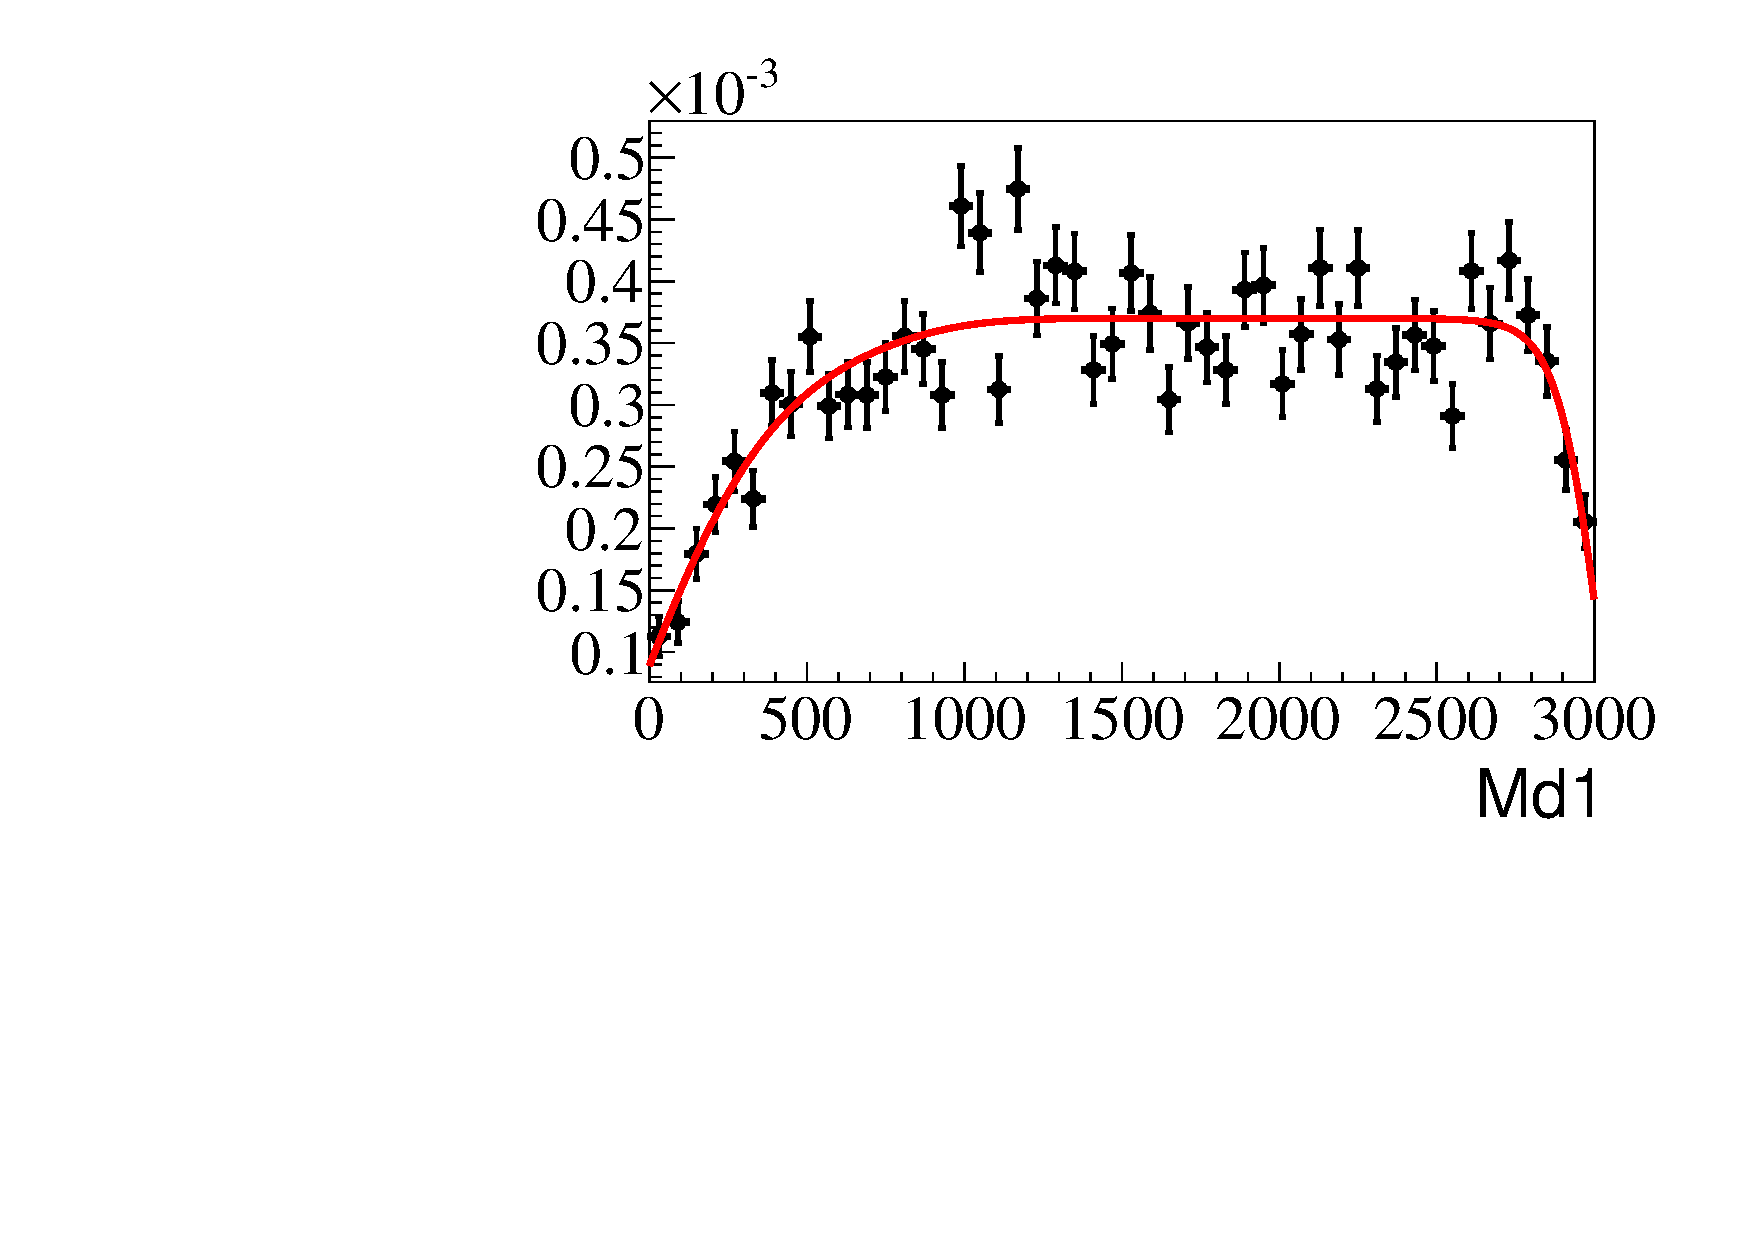
\includegraphics[width=50mm]{figures/pMSSMpaper/Prior/MLP/trainedRegression1_Md1}
}
\hspace{-8mm}
\subfloat[]{
  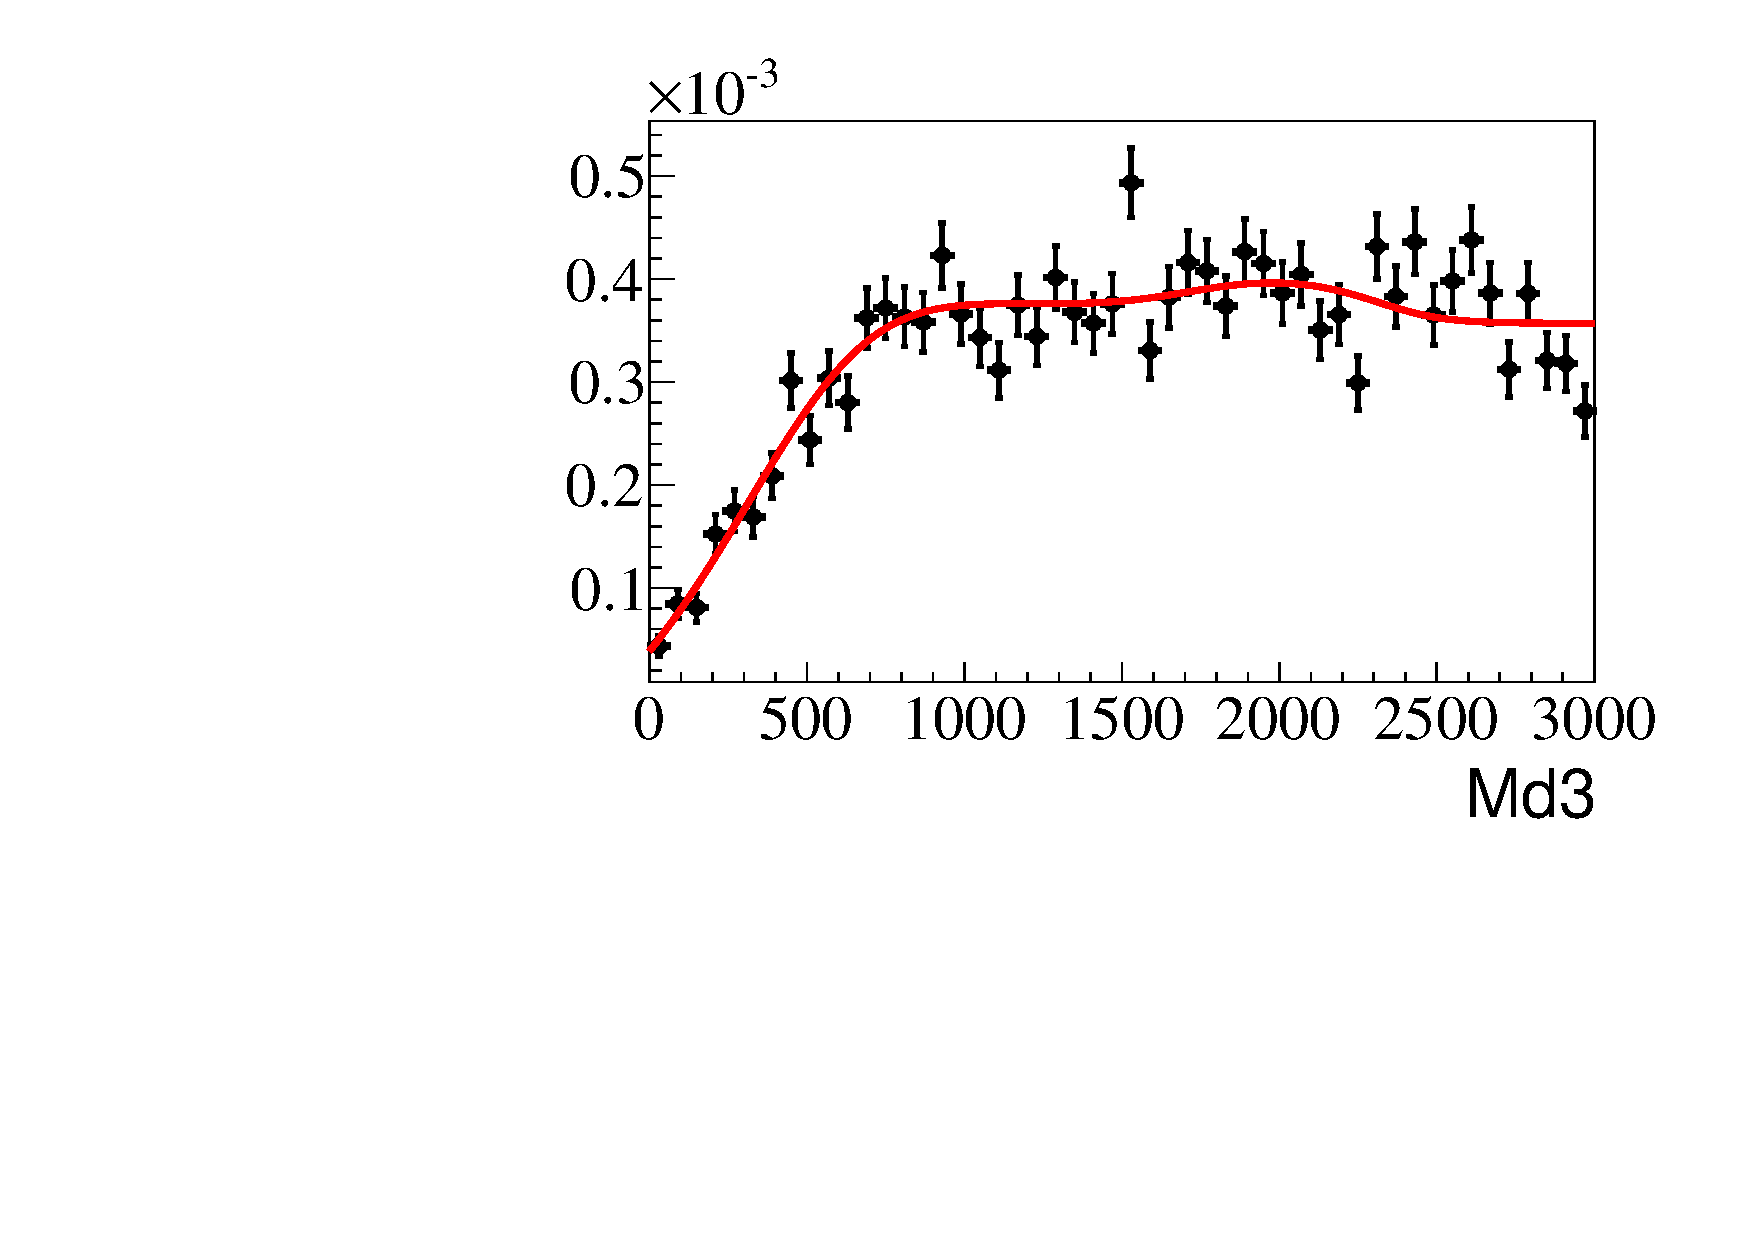
\includegraphics[width=50mm]{figures/pMSSMpaper/Prior/MLP/trainedRegression1_Md3}
}
\hspace{-8mm}
\subfloat[]{
  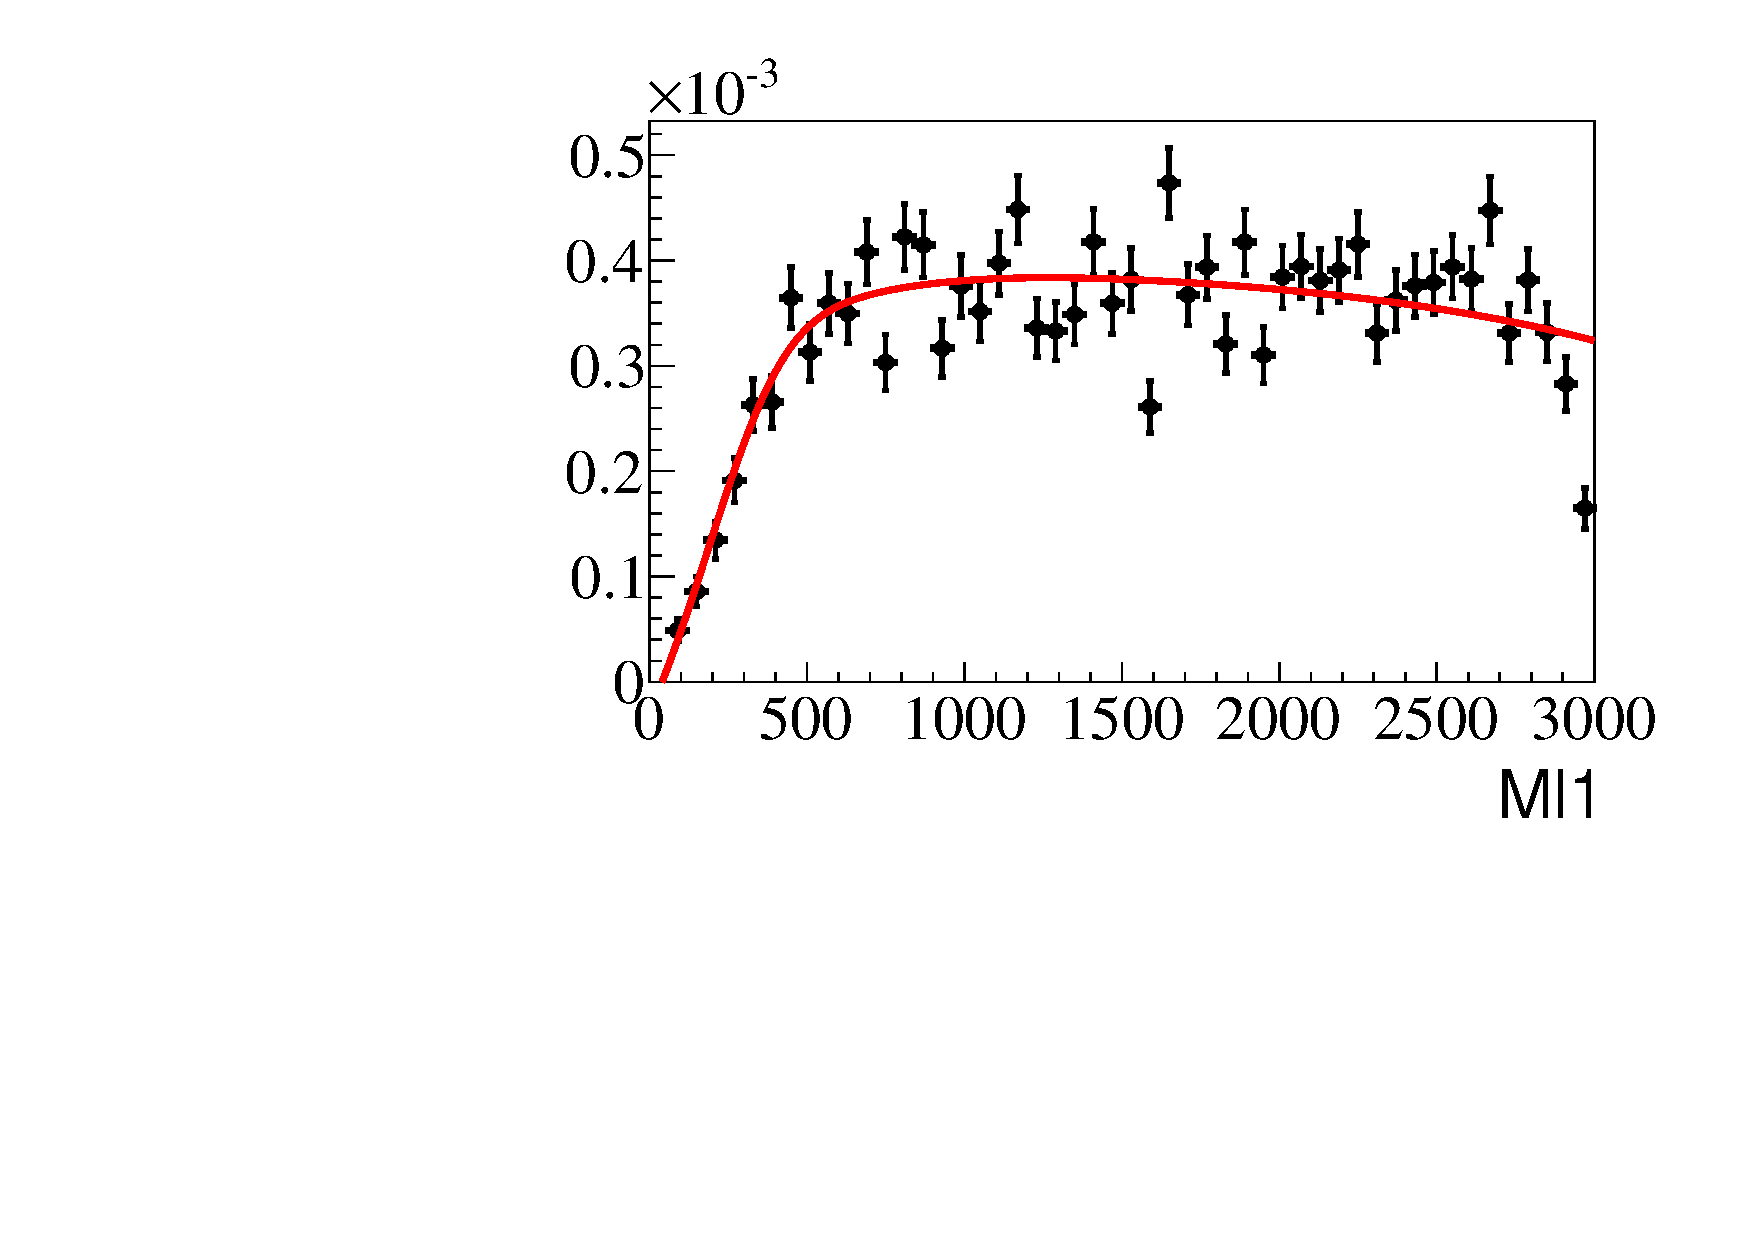
\includegraphics[width=50mm]{figures/pMSSMpaper/Prior/MLP/trainedRegression1_Ml1}
}
\hspace{-8mm}
\subfloat[]{
  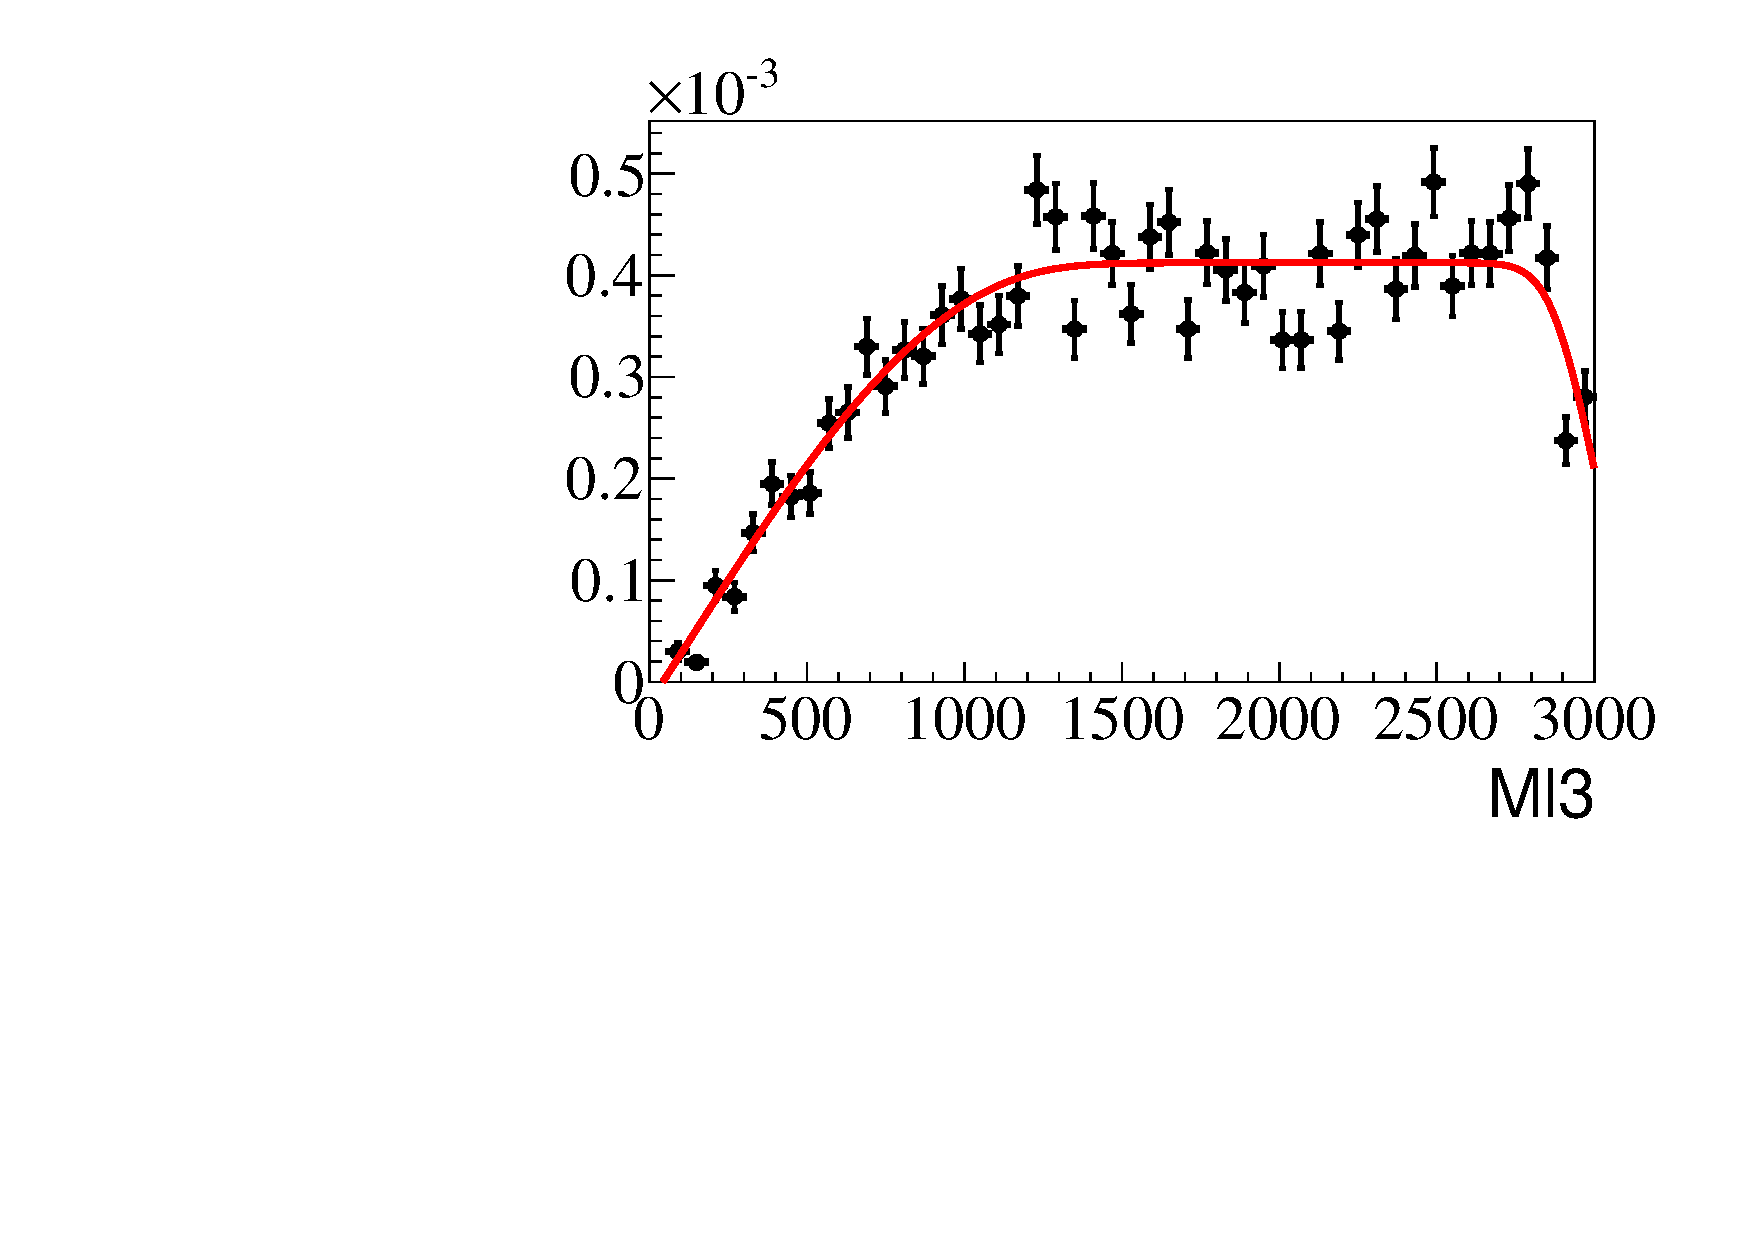
\includegraphics[width=50mm]{figures/pMSSMpaper/Prior/MLP/trainedRegression1_Ml3}
}
\hspace{-8mm}
\subfloat[]{
  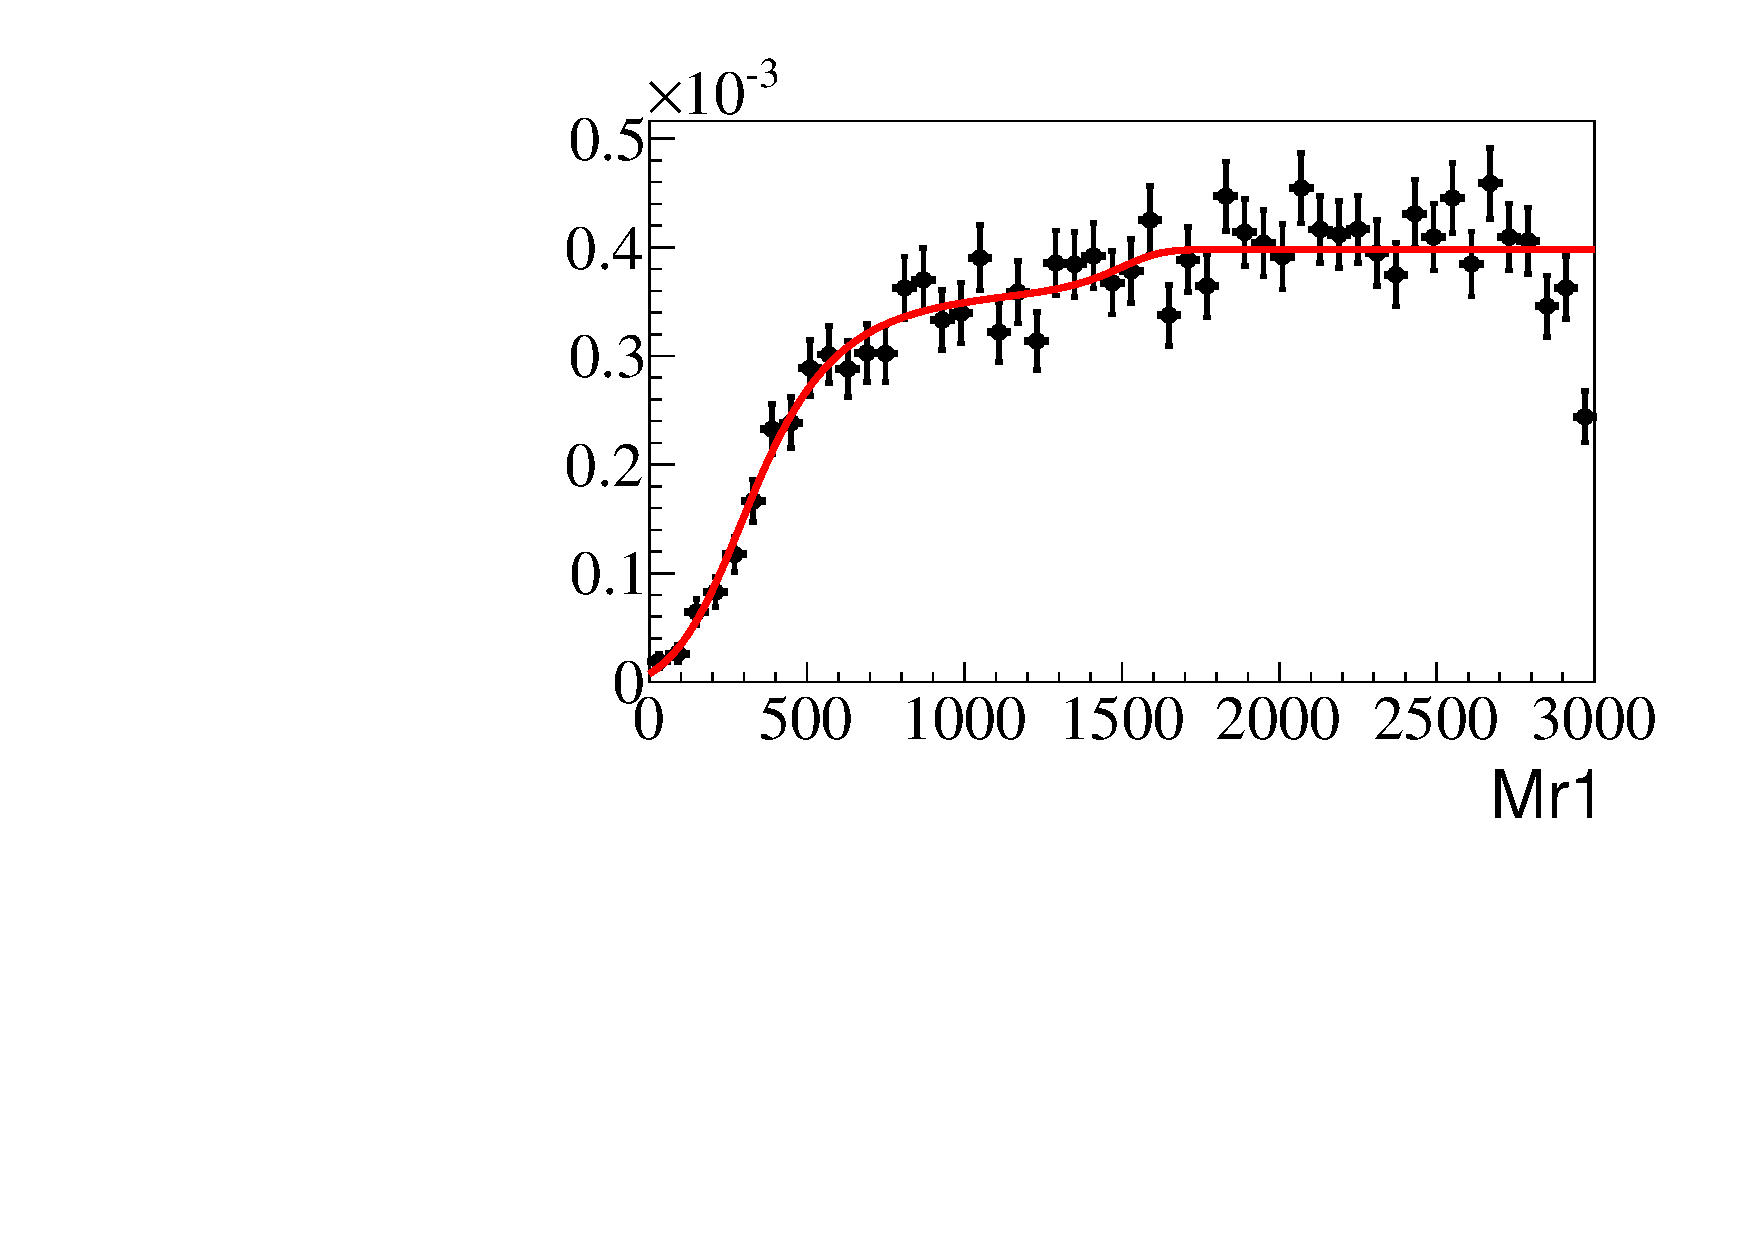
\includegraphics[width=50mm]{figures/pMSSMpaper/Prior/MLP/trainedRegression1_Mr1}
}
\hspace{-8mm}
\subfloat[]{
  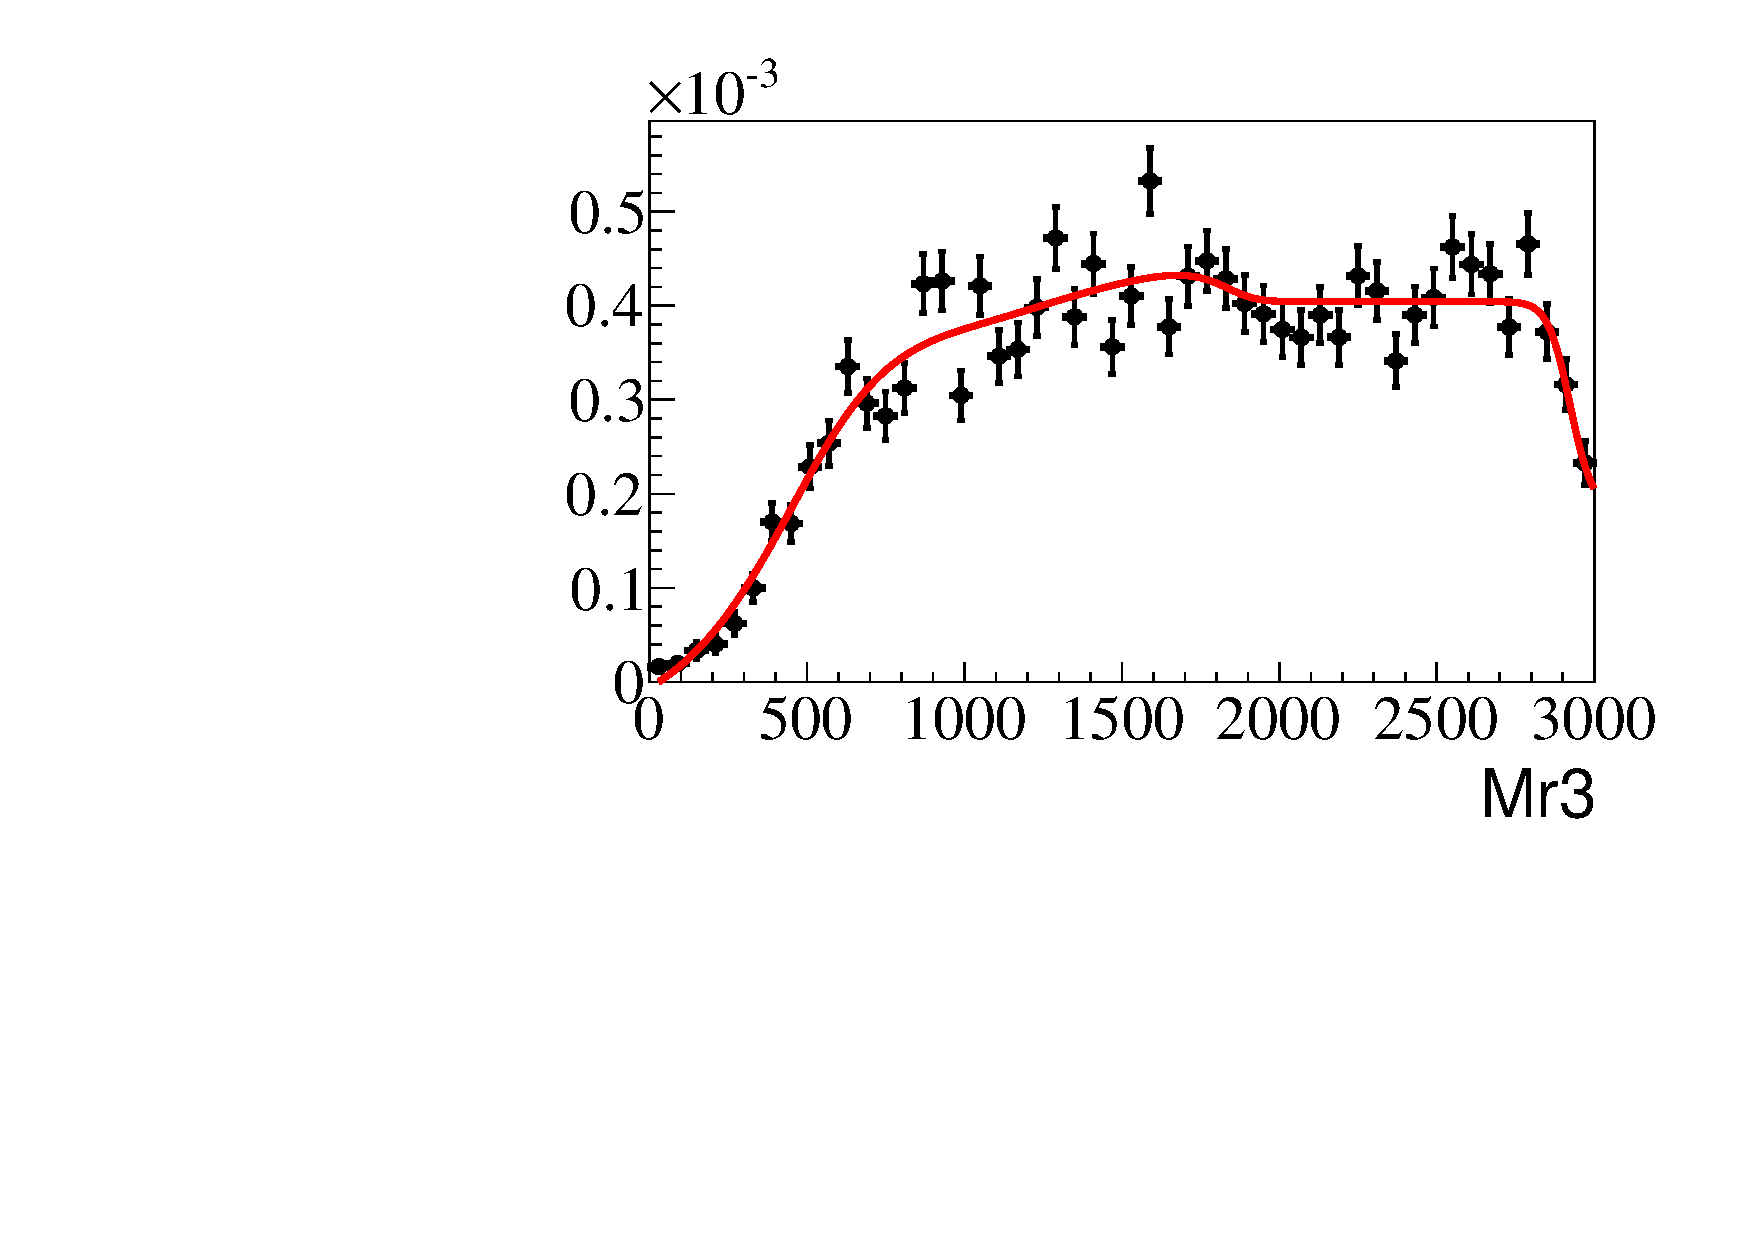
\includegraphics[width=50mm]{figures/pMSSMpaper/Prior/MLP/trainedRegression1_Mr3}
}
\hspace{-8mm}
\subfloat[]{
  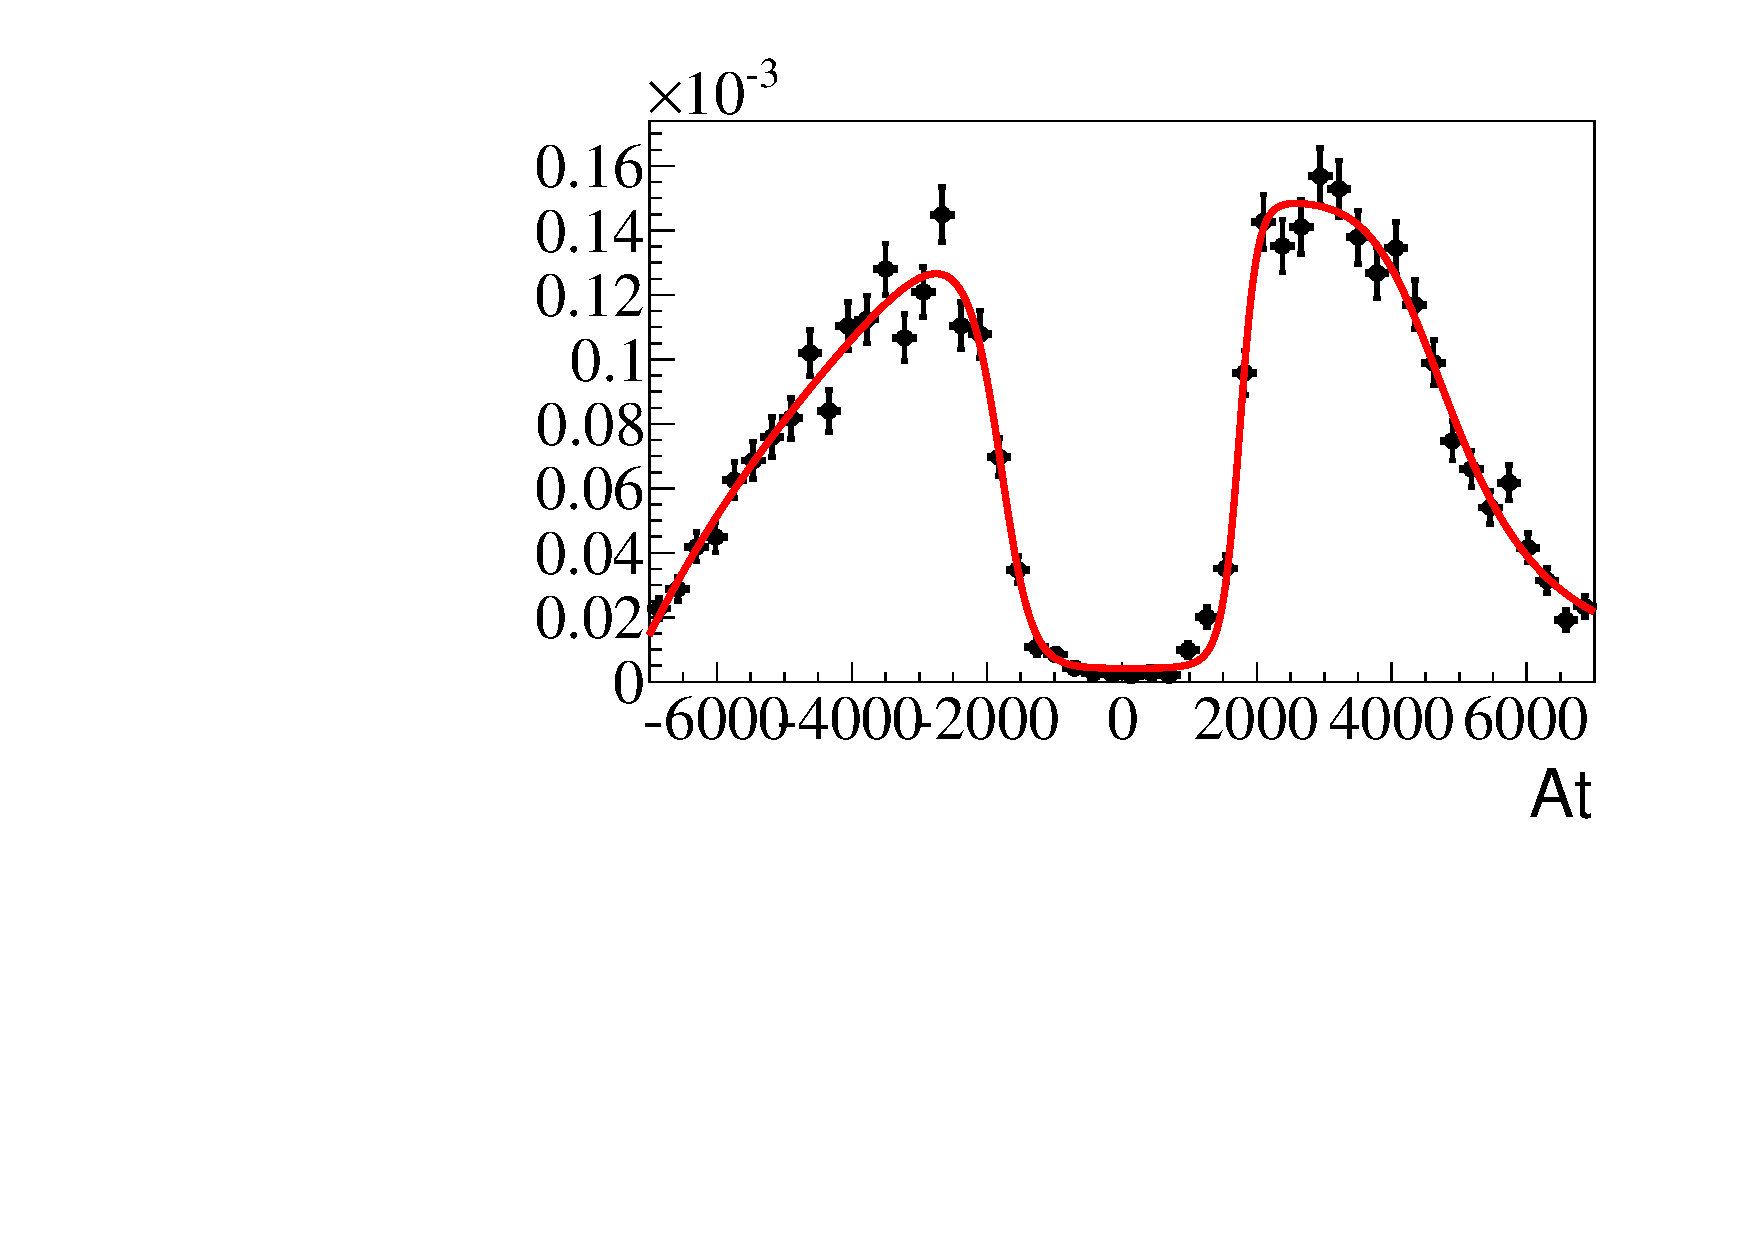
\includegraphics[width=50mm]{figures/pMSSMpaper/Prior/MLP/trainedRegression1_At}
}
\hspace{-8mm}
\subfloat[]{
  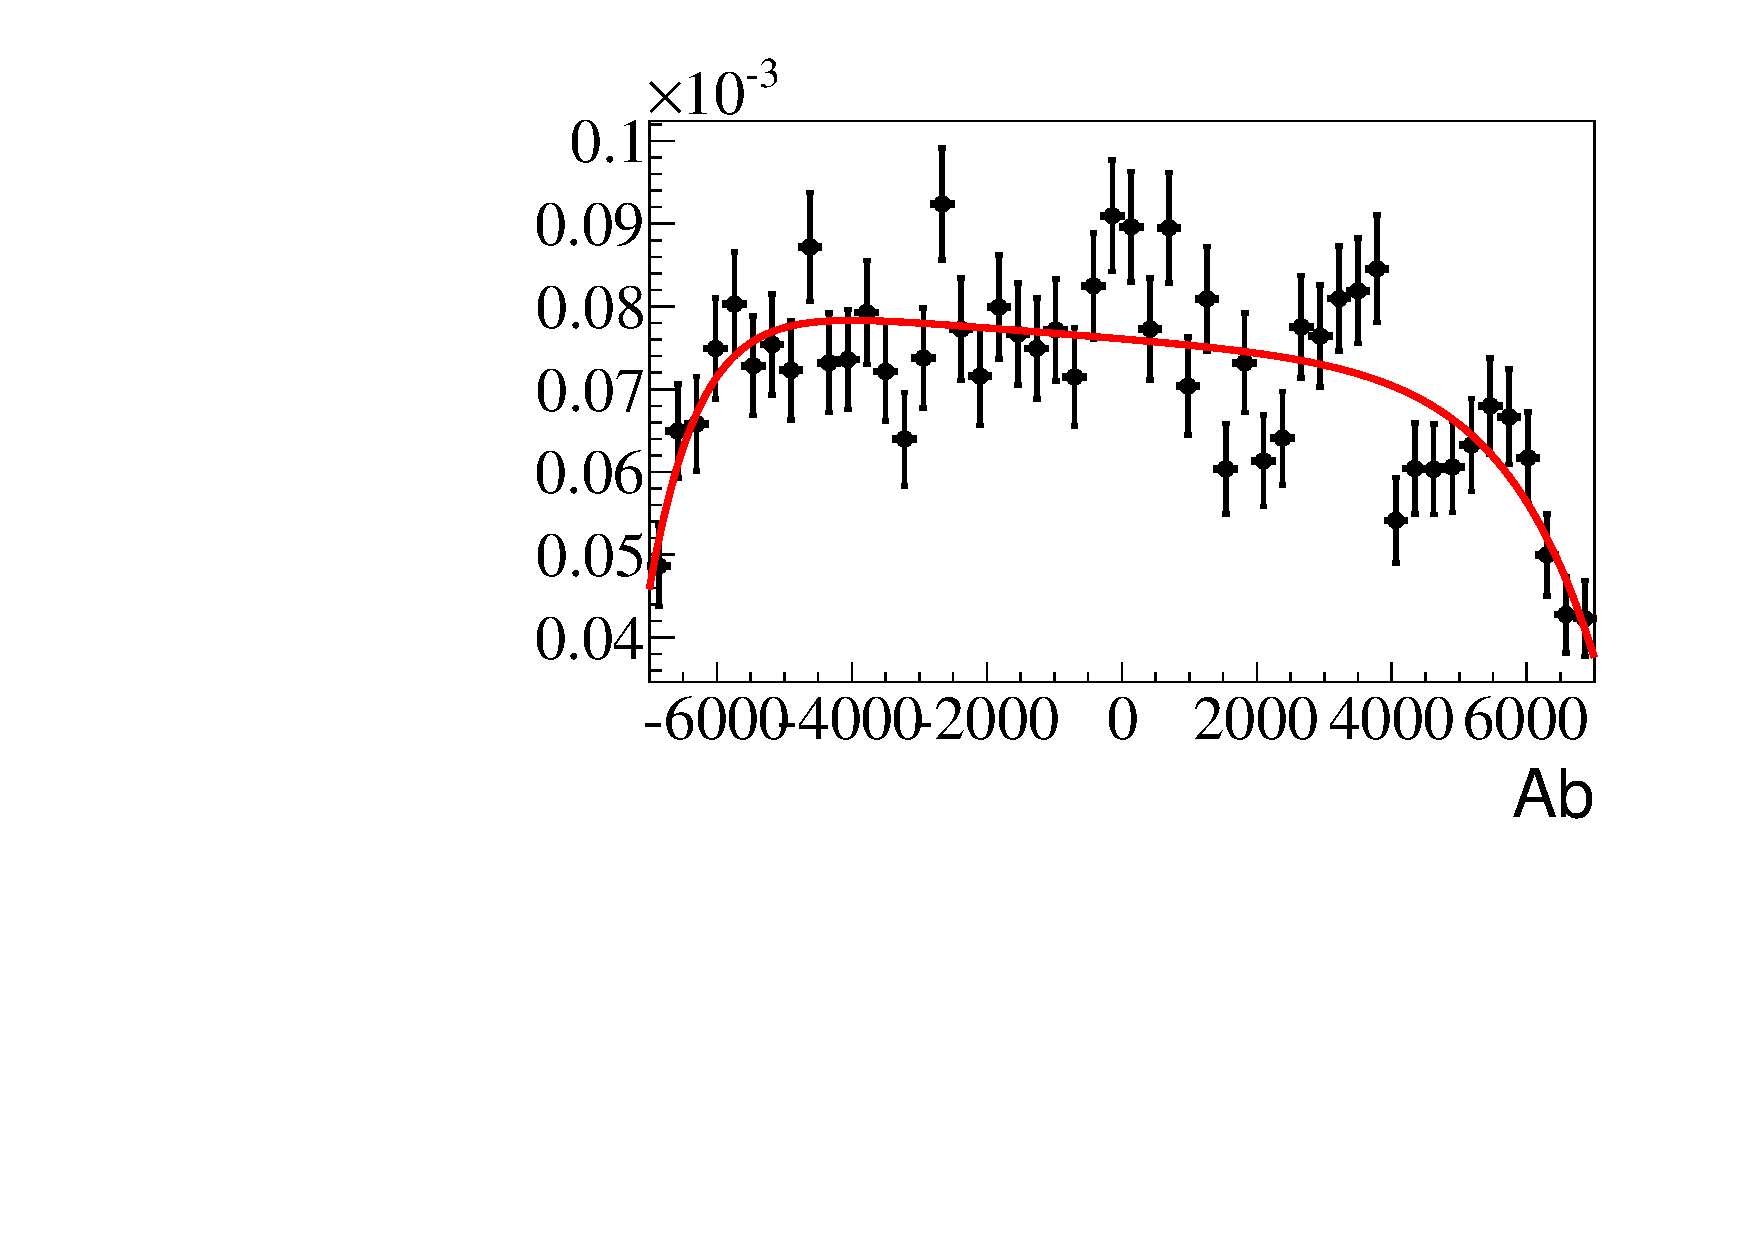
\includegraphics[width=50mm]{figures/pMSSMpaper/Prior/MLP/trainedRegression1_Ab}
}
\hspace{-8mm}
\subfloat[]{
  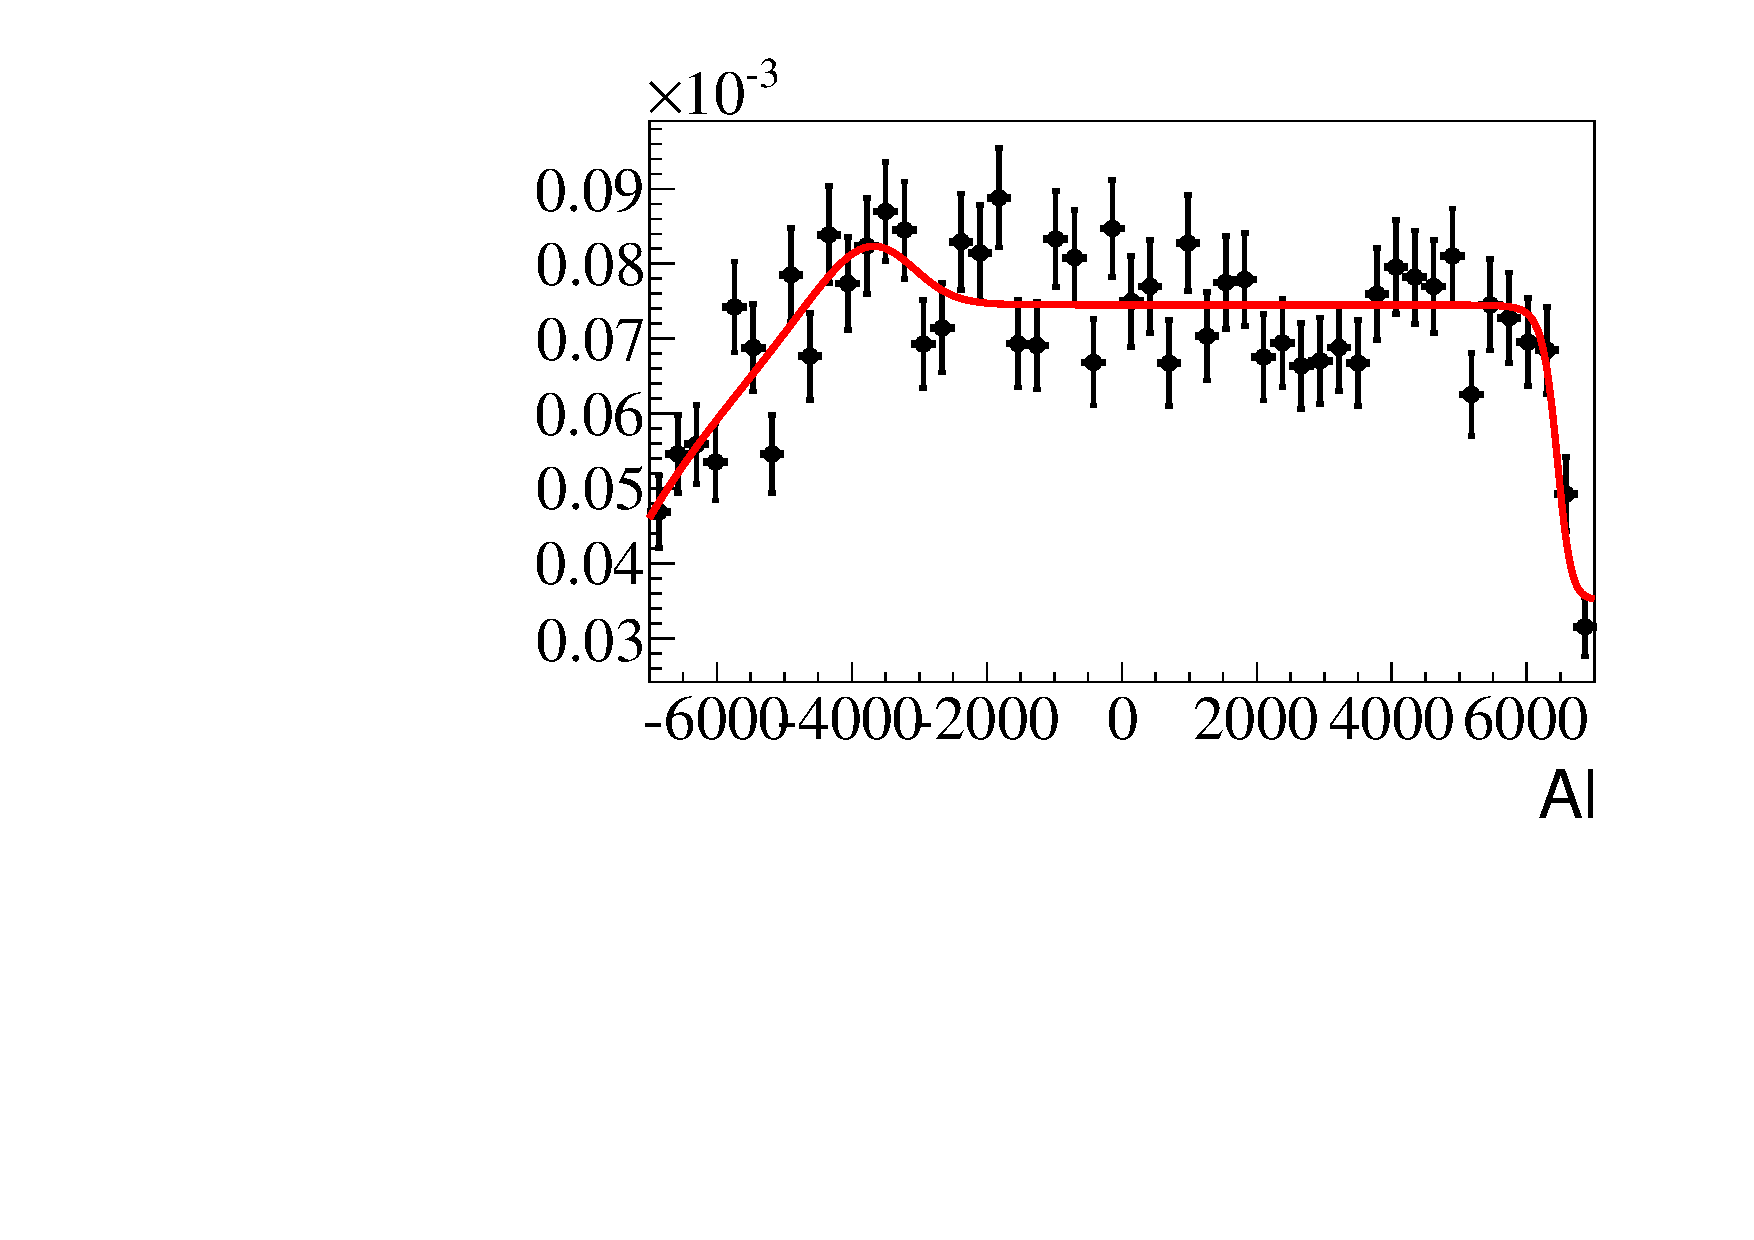
\includegraphics[width=50mm]{figures/pMSSMpaper/Prior/MLP/trainedRegression1_Al}
}
\caption{The results of the 19 MLP regressions on the pMSSM parameters. }
\label{fig:KdeMlp}
\end{figure}
\FloatBarrier

\begin{figure}[h]
\centering
  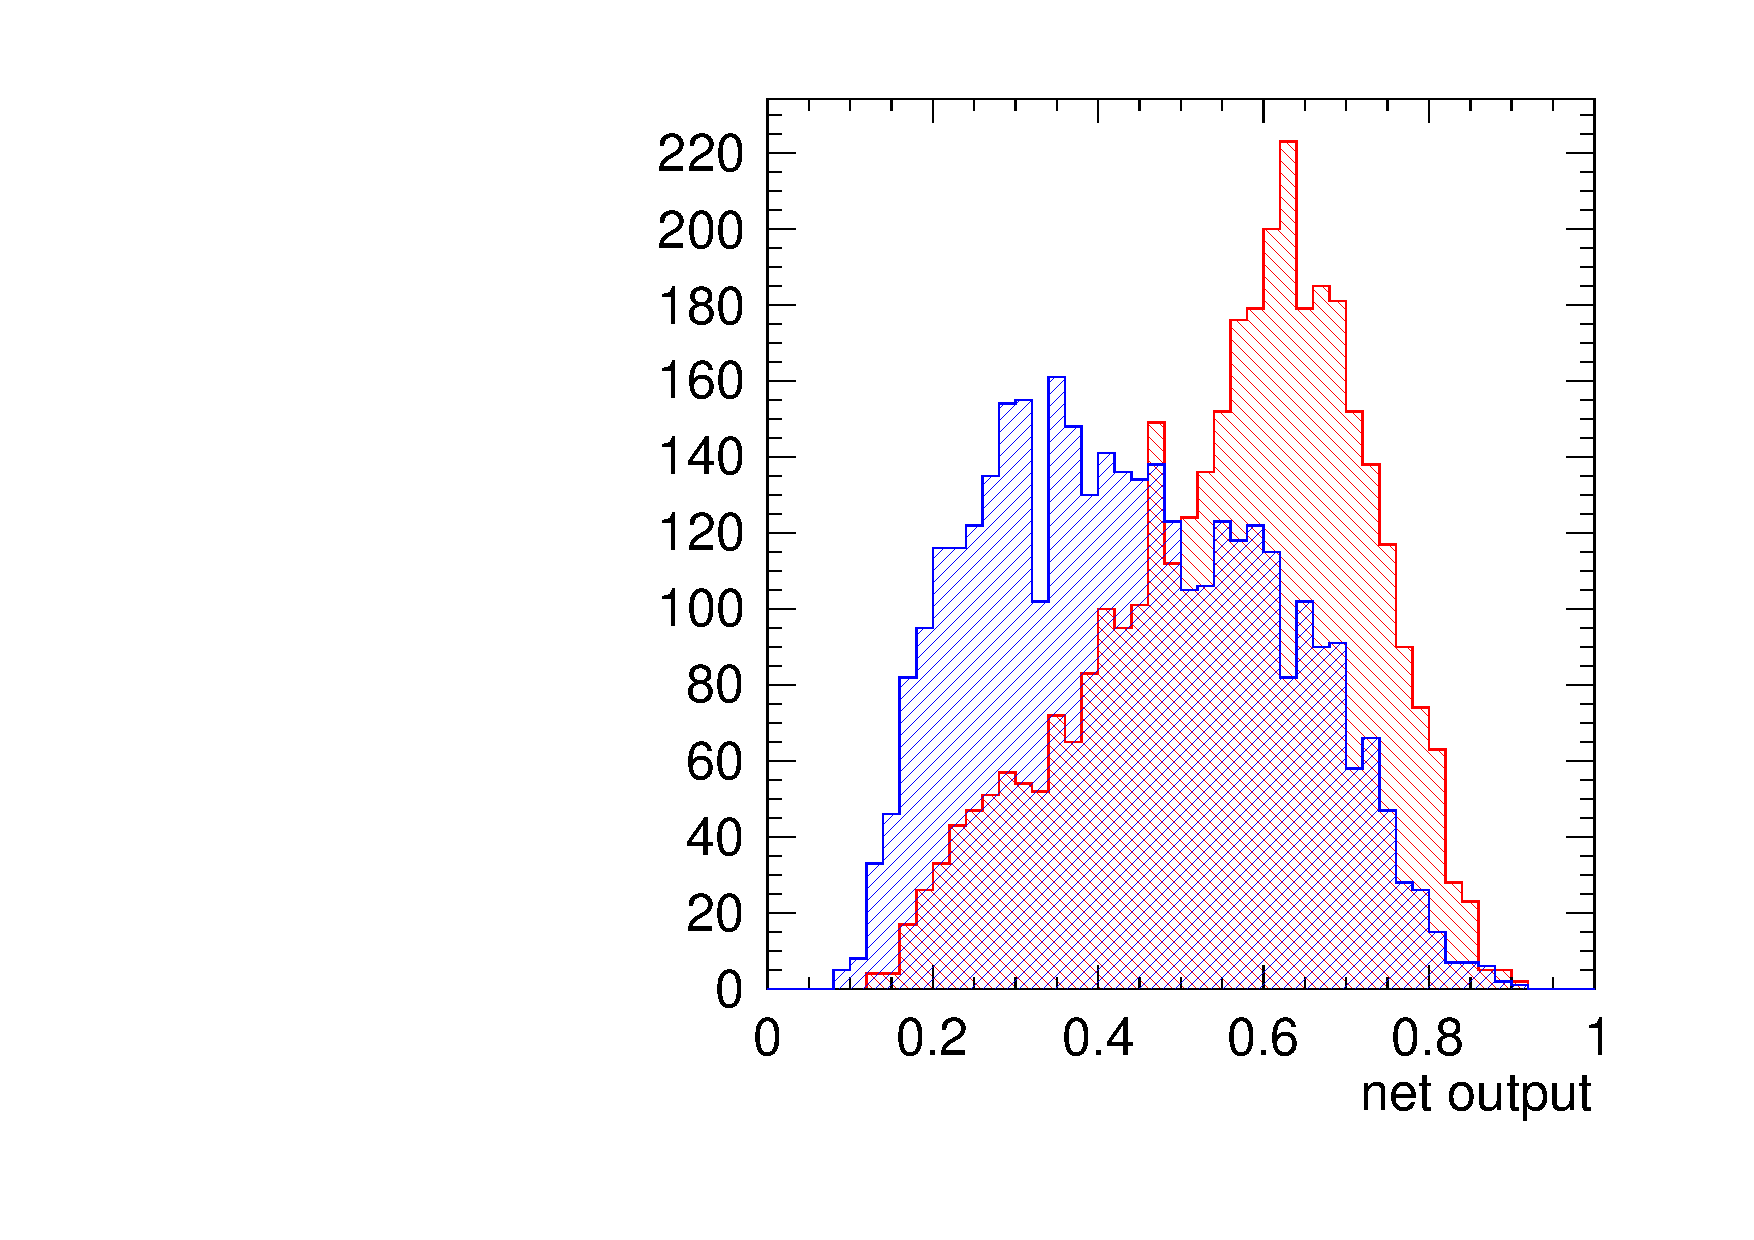
\includegraphics[width=0.6\linewidth]{figures/pMSSMpaper/Prior/CompareFrequentist/figpmssmnettrain}
\caption{The output of the MLP used to derive the correction function. The red distribution is the original set of pMSSM points and the blue distribution is the set generated by a random sampling of the separable likelihood function. }
\label{fig:Classifier}
\end{figure}

%\begin{figure}[h]
%\centering
%\subfloat[]{
%  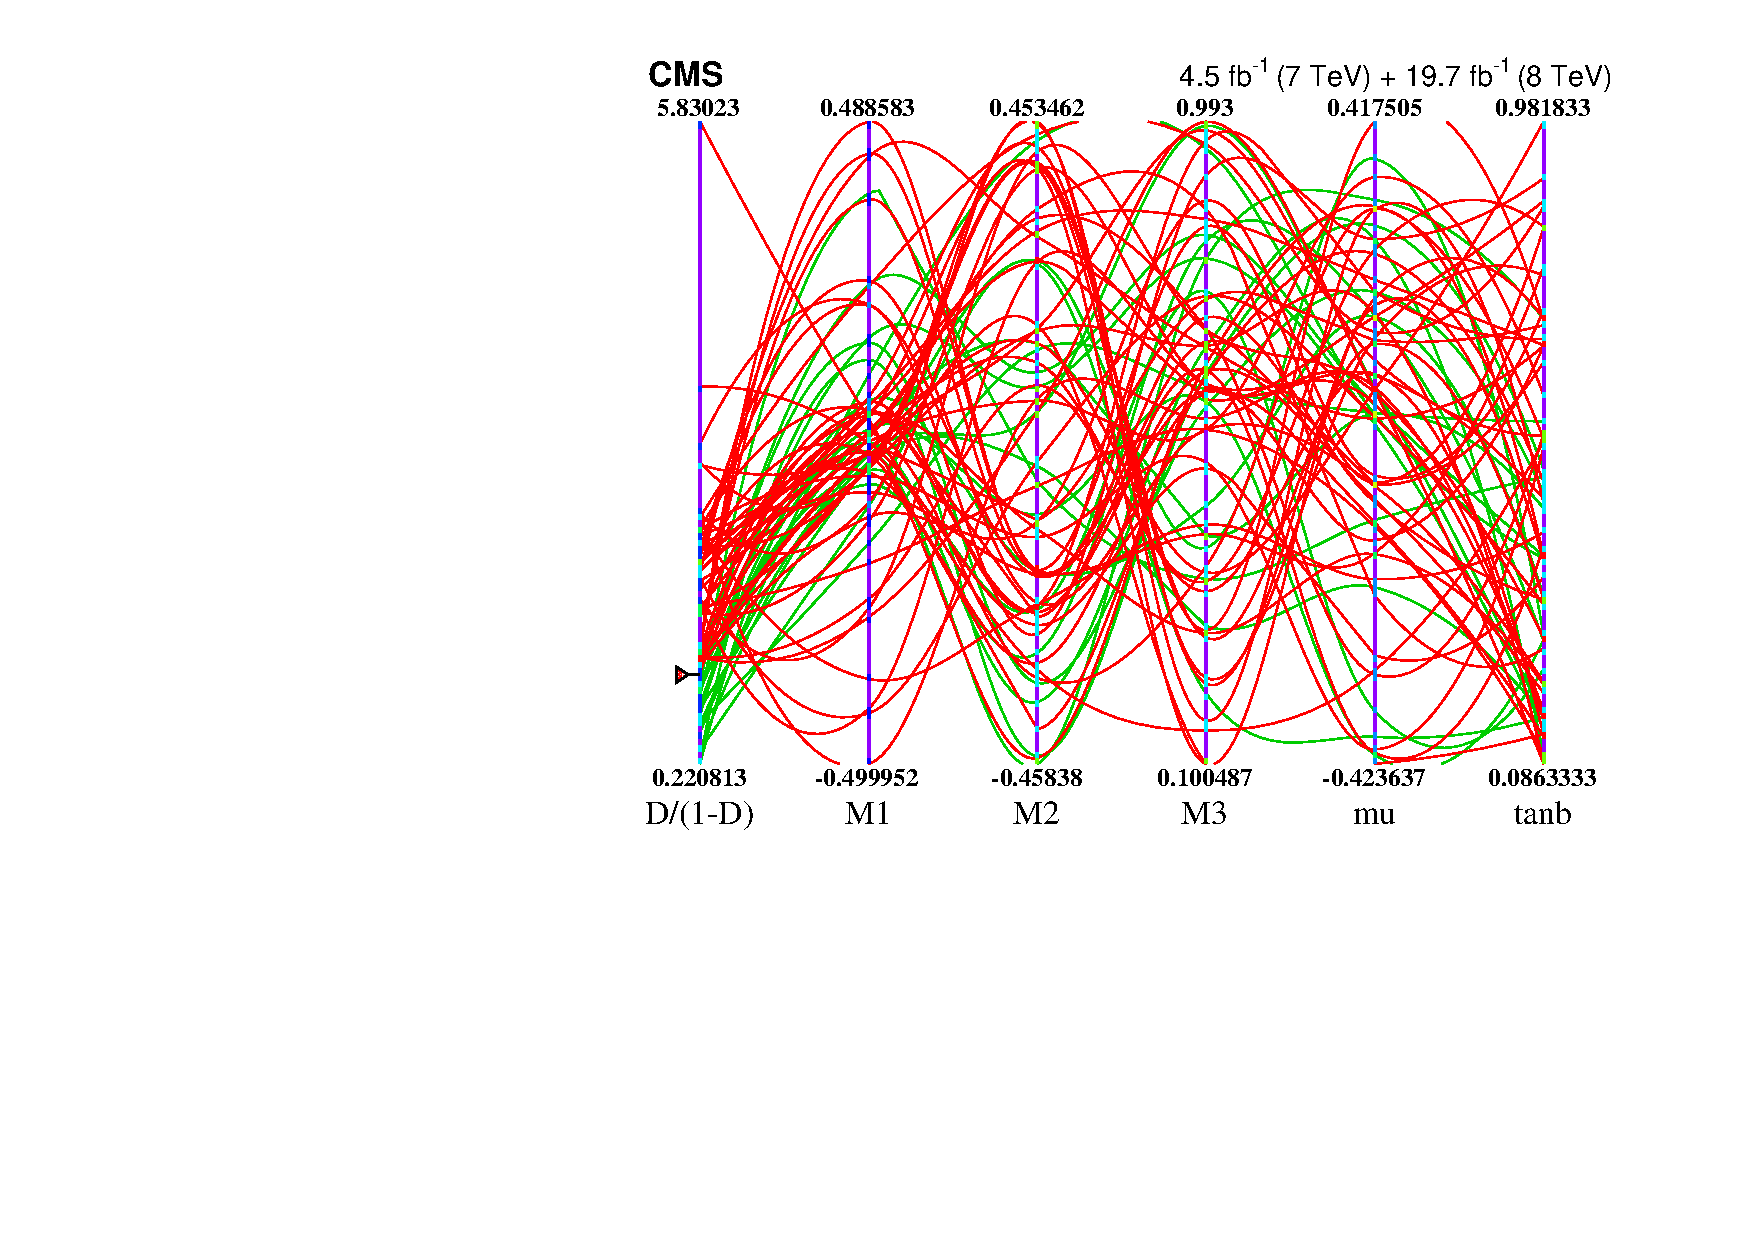
\includegraphics[width=0.9\linewidth]{figures/pMSSMpaper/Prior/CompareFrequentist/ParCorCorrFunction.pdf}
%  }
%\caption{A parallel coordinates plot of showing the correlation function D/(1-D) and its dependence on a few pMSSM parameters. The correlation function is not dominantly correlated with any one variable. The pMSSM parameters have each been normalized to a unit interval.}
%\label{fig:LlhdVs19dMva}
%\end{figure}


\renewcommand*\thesubfigure{\arabic{subfigure}}
\begin{figure}[htbp]
\centering
\hspace{2mm}
\subfloat[]{
  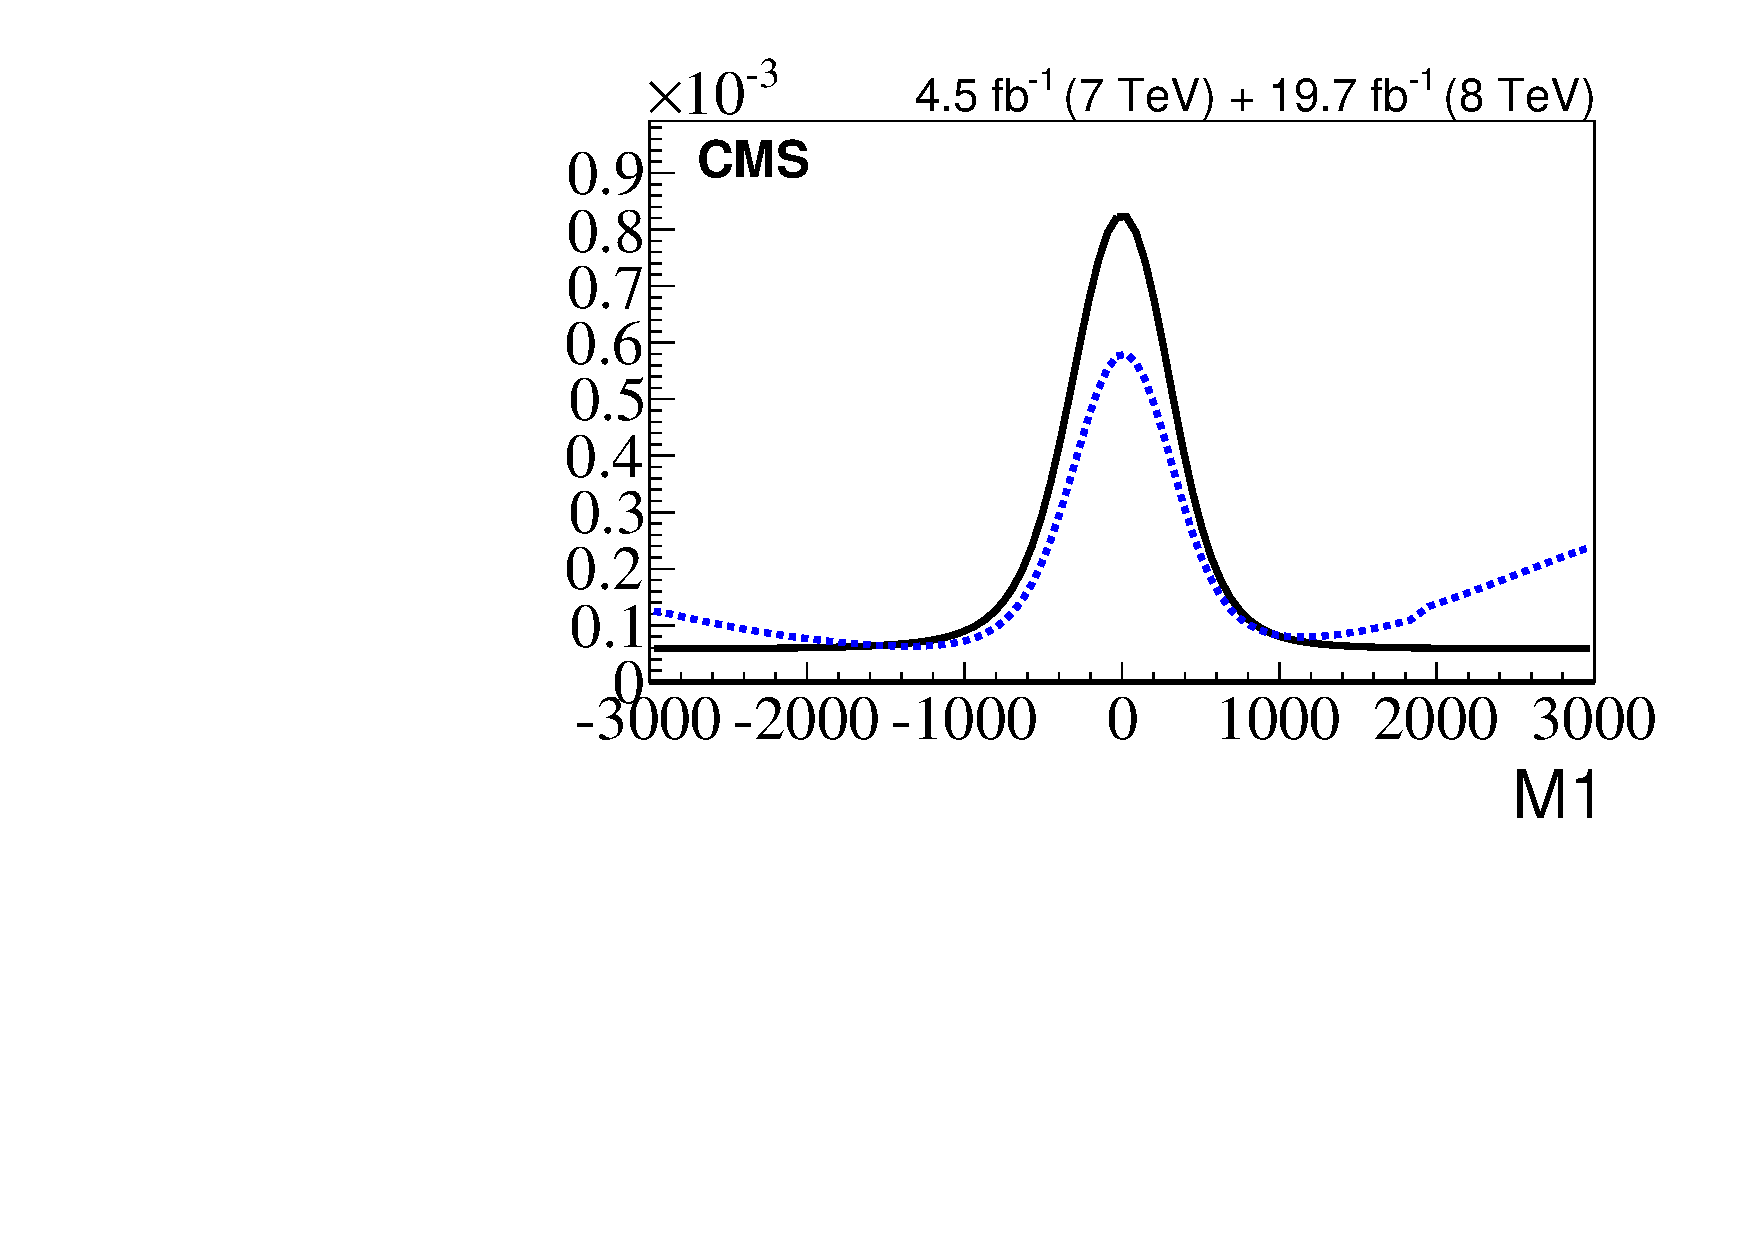
\includegraphics[width=65mm]{figures/pMSSMpaper/Prior/CompareFrequentist/CompareProfileLhdWithPriorM1}
}
\hspace{2mm}
\subfloat[]{
  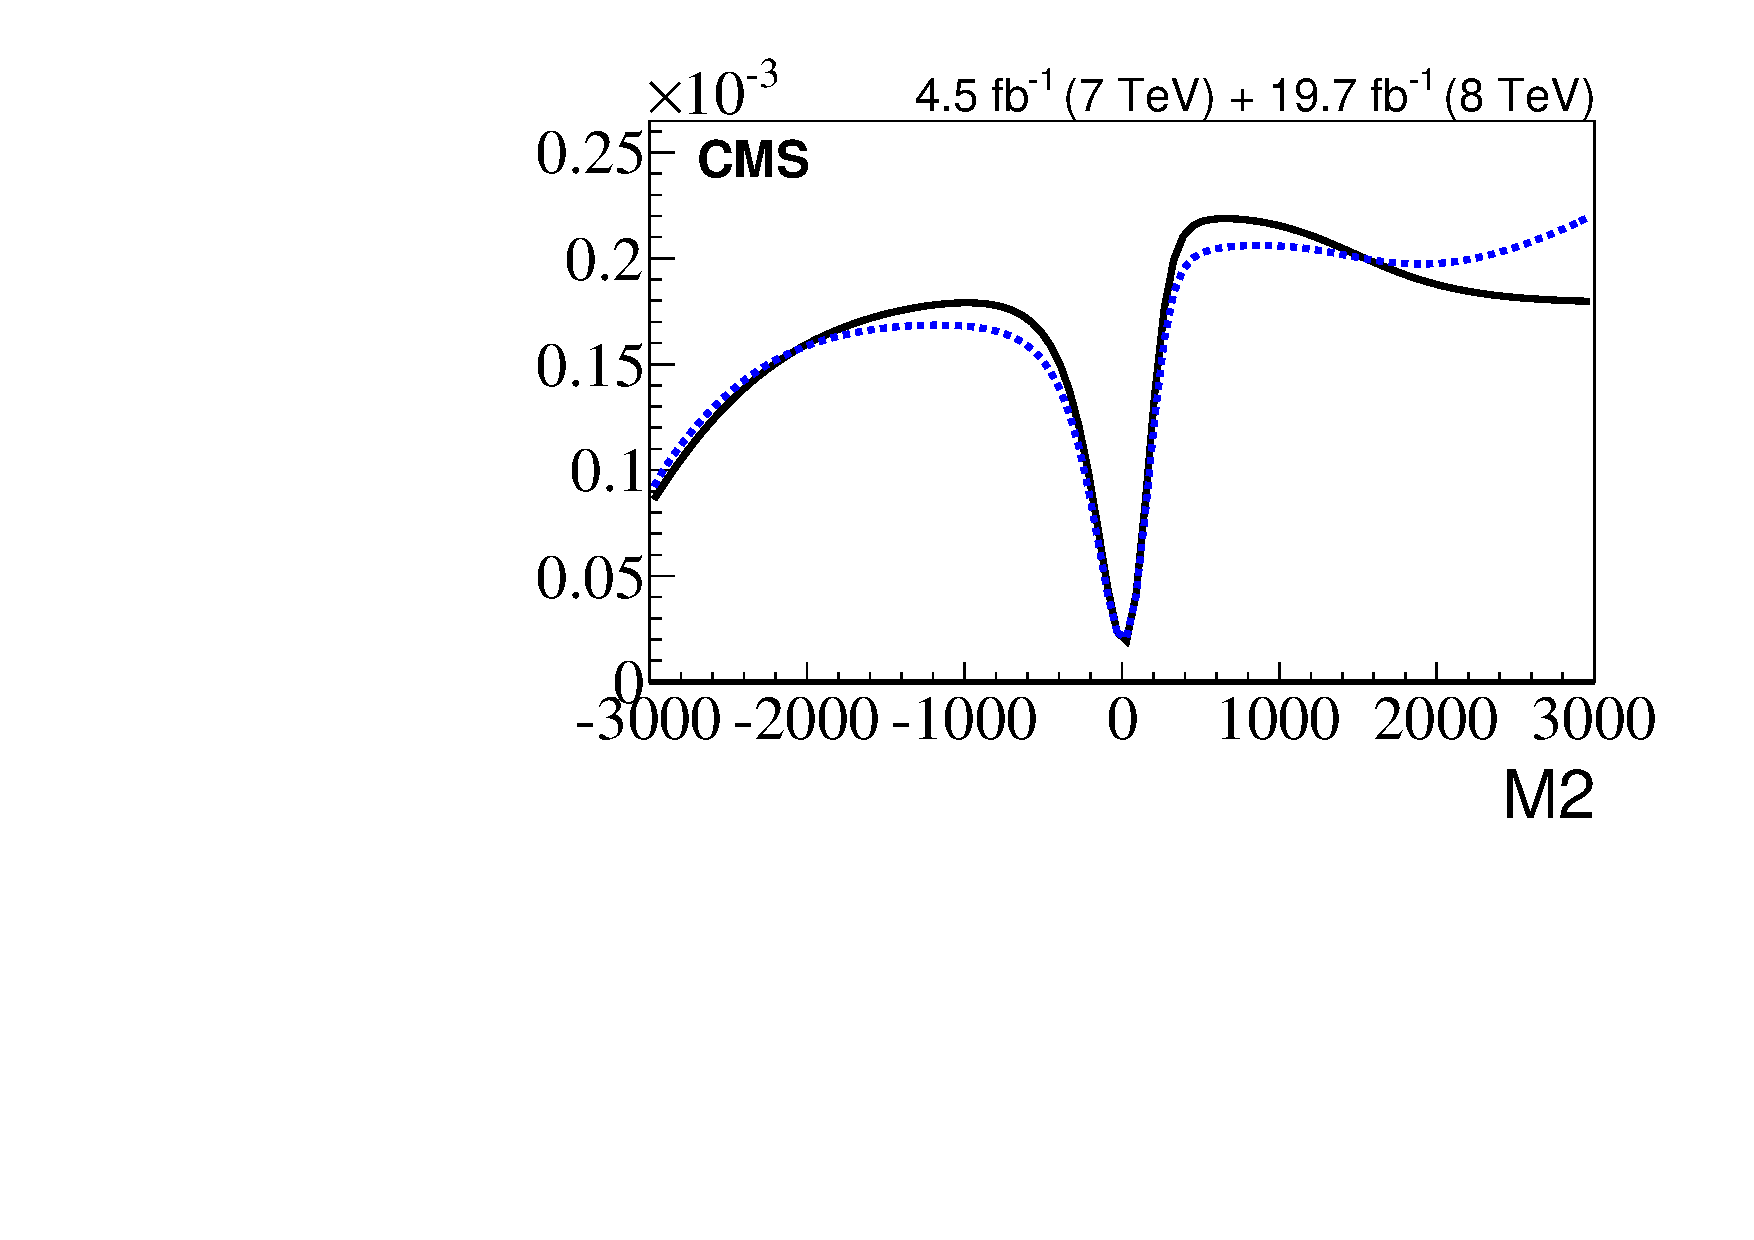
\includegraphics[width=65mm]{figures/pMSSMpaper/Prior/CompareFrequentist/CompareProfileLhdWithPriorM2}
}
\hspace{2mm}
\subfloat[]{
  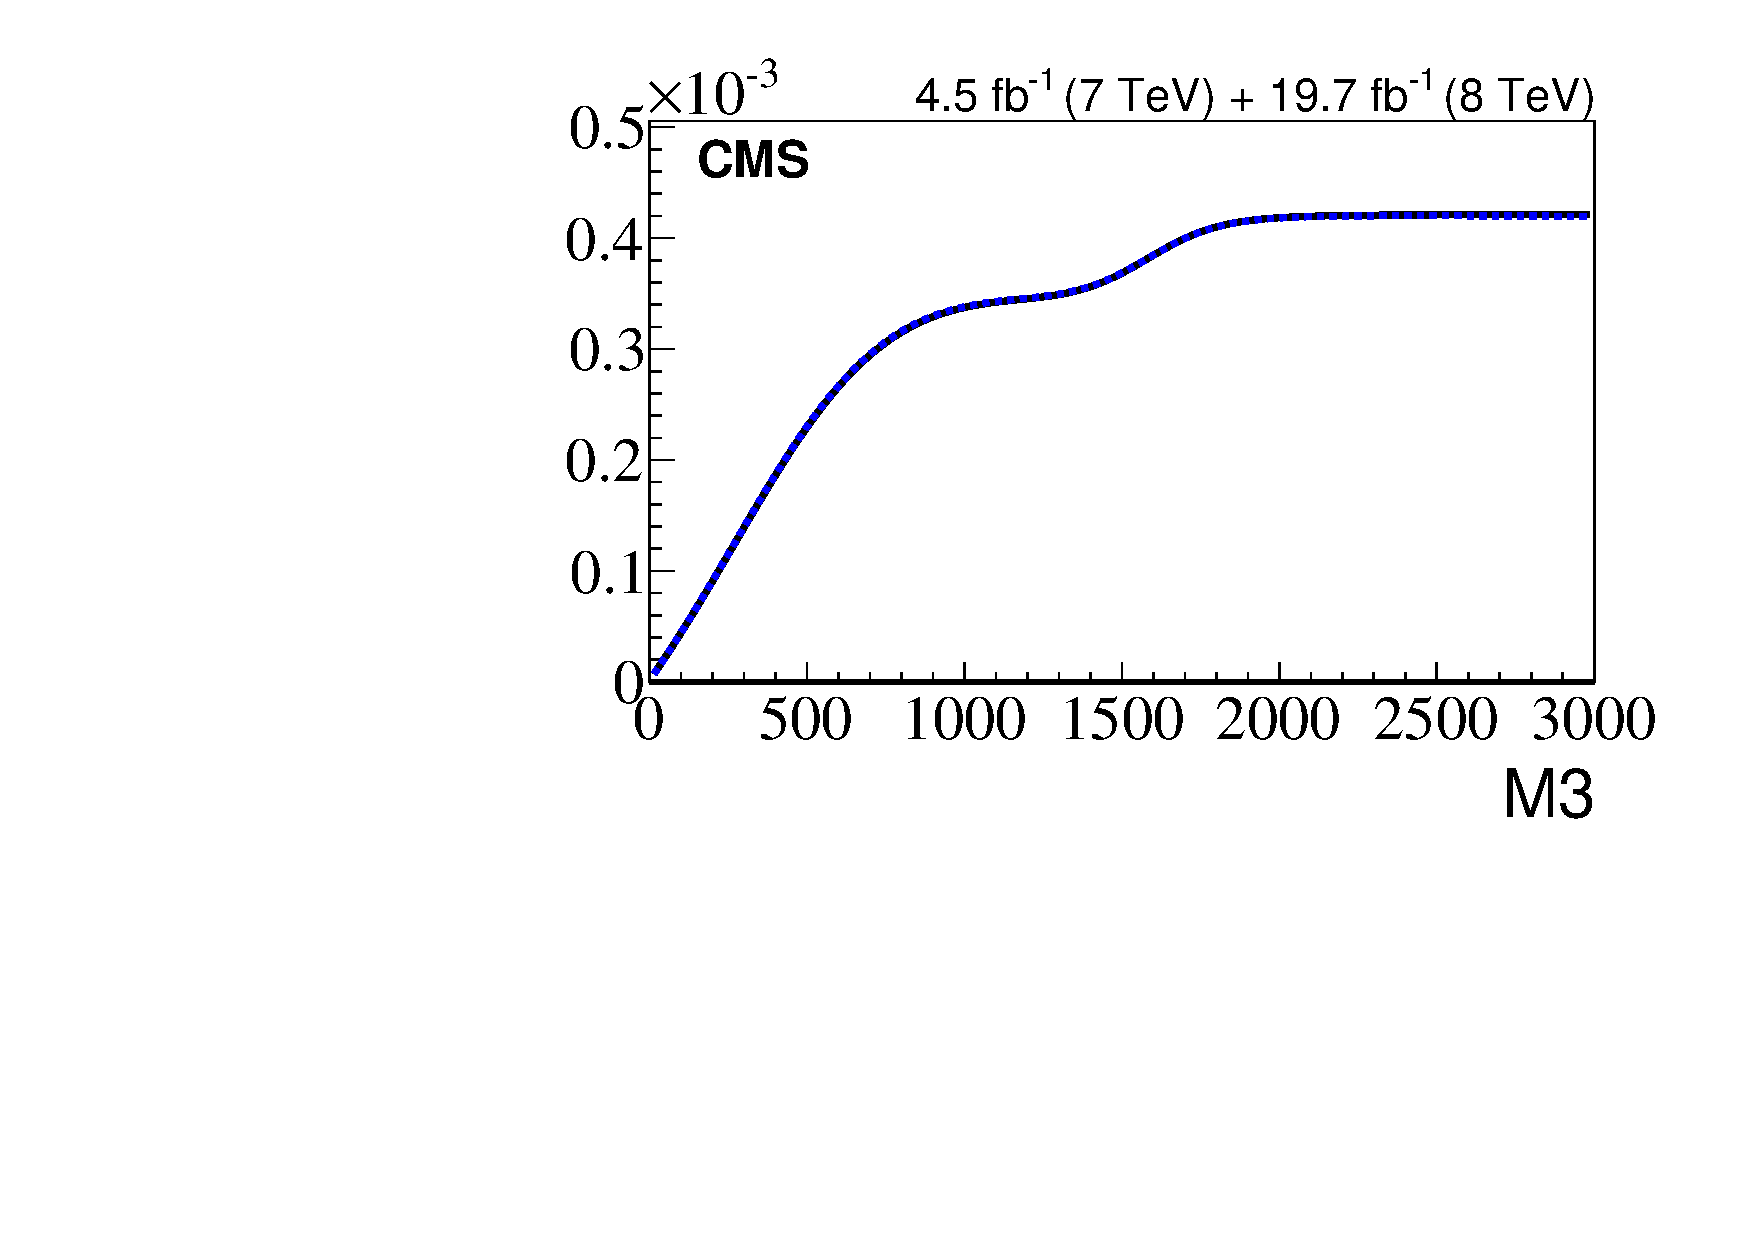
\includegraphics[width=65mm]{figures/pMSSMpaper/Prior/CompareFrequentist/CompareProfileLhdWithPriorM3}
}
\hspace{2mm}
\subfloat[]{
  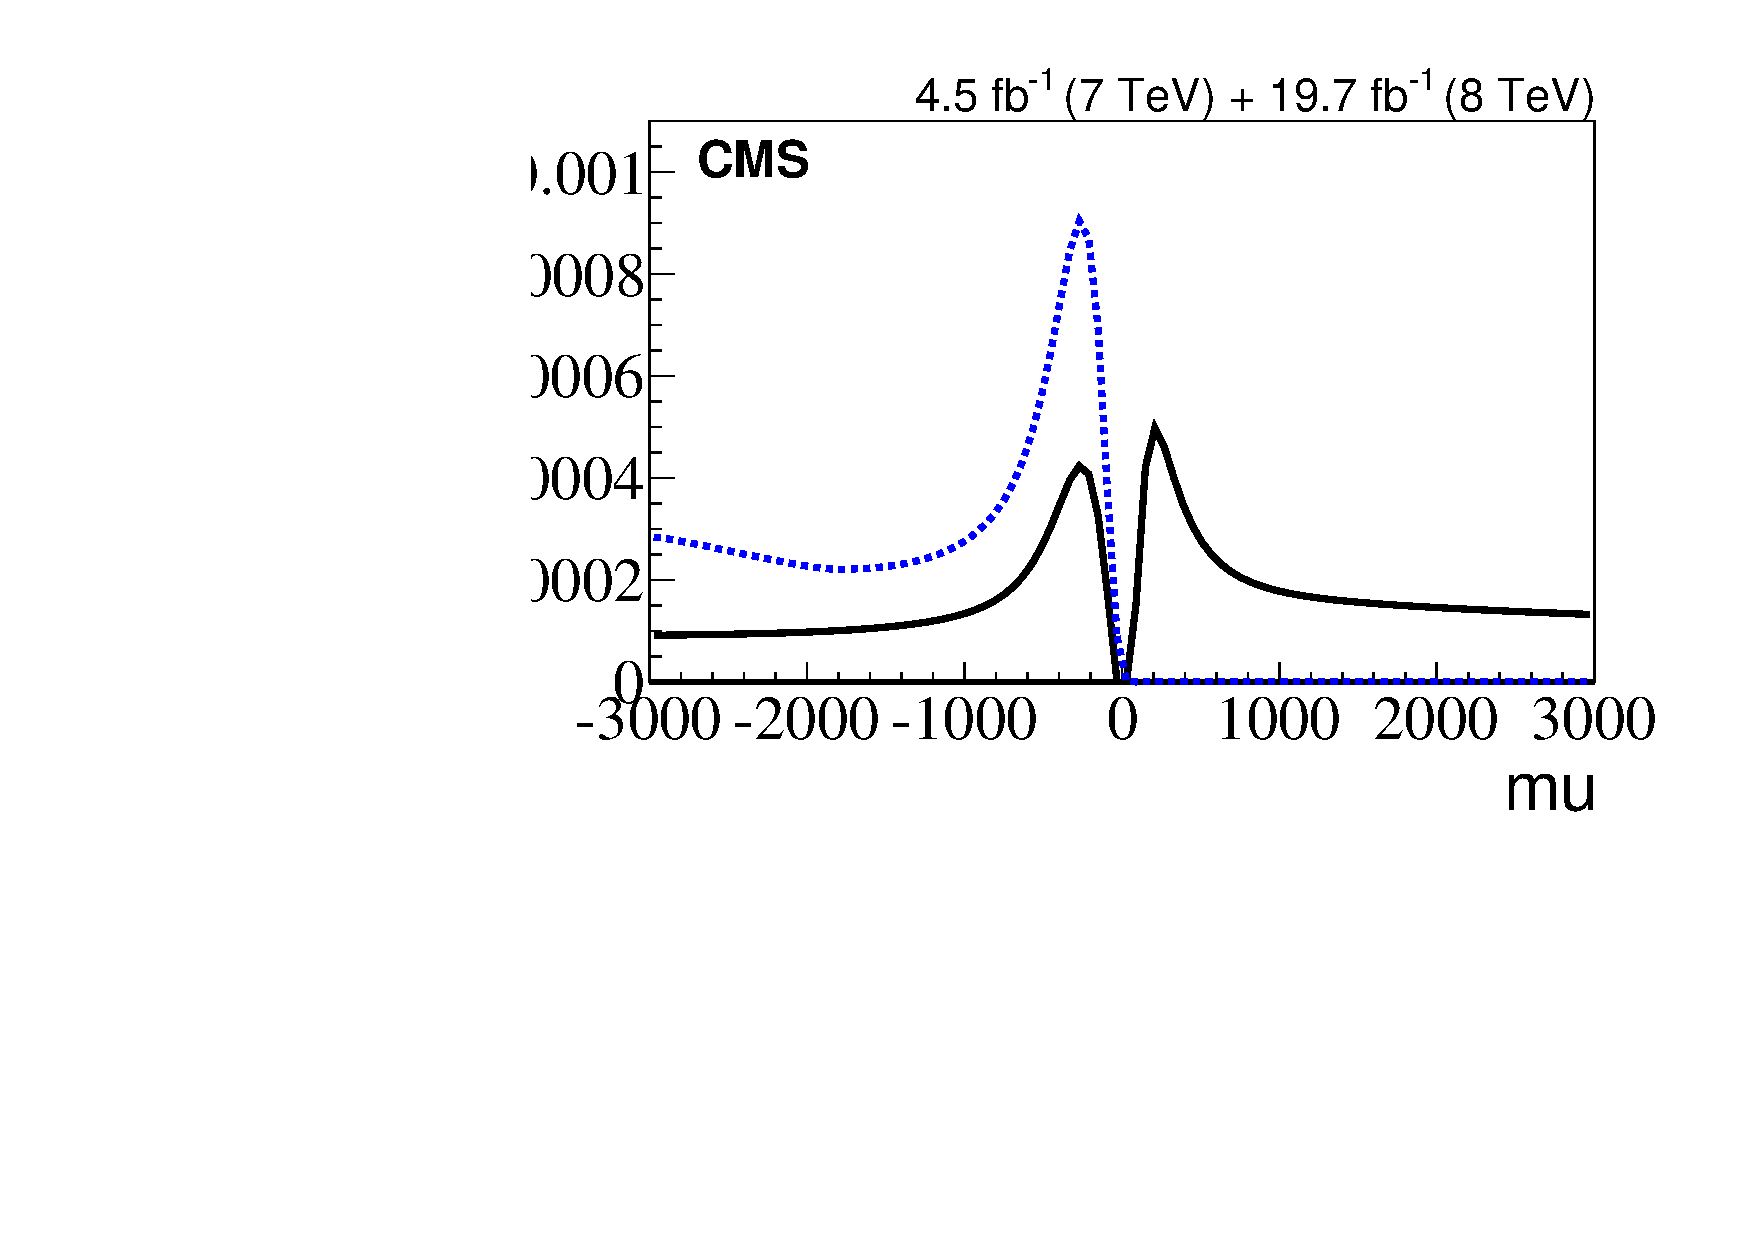
\includegraphics[width=65mm]{figures/pMSSMpaper/Prior/CompareFrequentist/CompareProfileLhdWithPriormu}
}
\hspace{2mm}
\subfloat[]{   % ???
  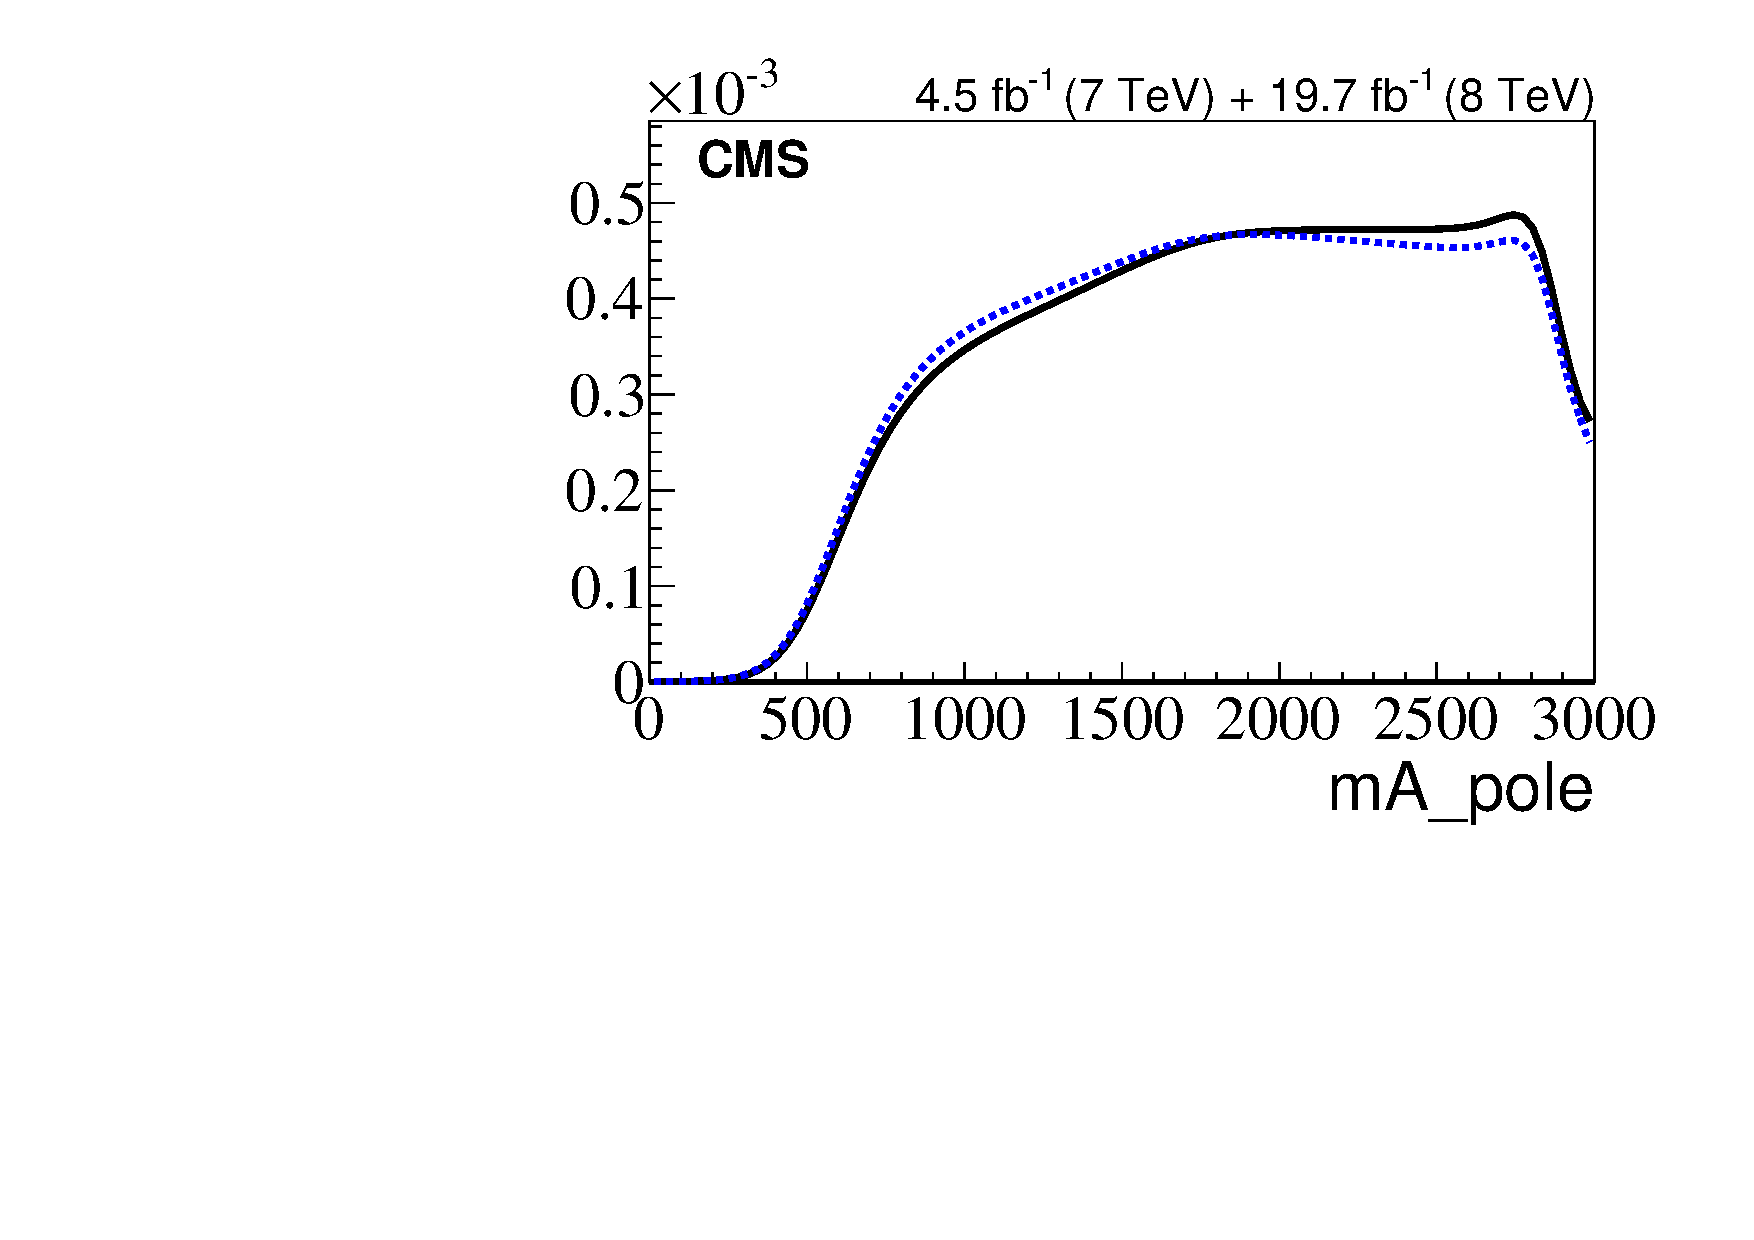
\includegraphics[width=65mm]{figures/pMSSMpaper/Prior/CompareFrequentist/CompareProfileLhdWithPriormApole}
}
\hspace{2mm}
\subfloat[]{
  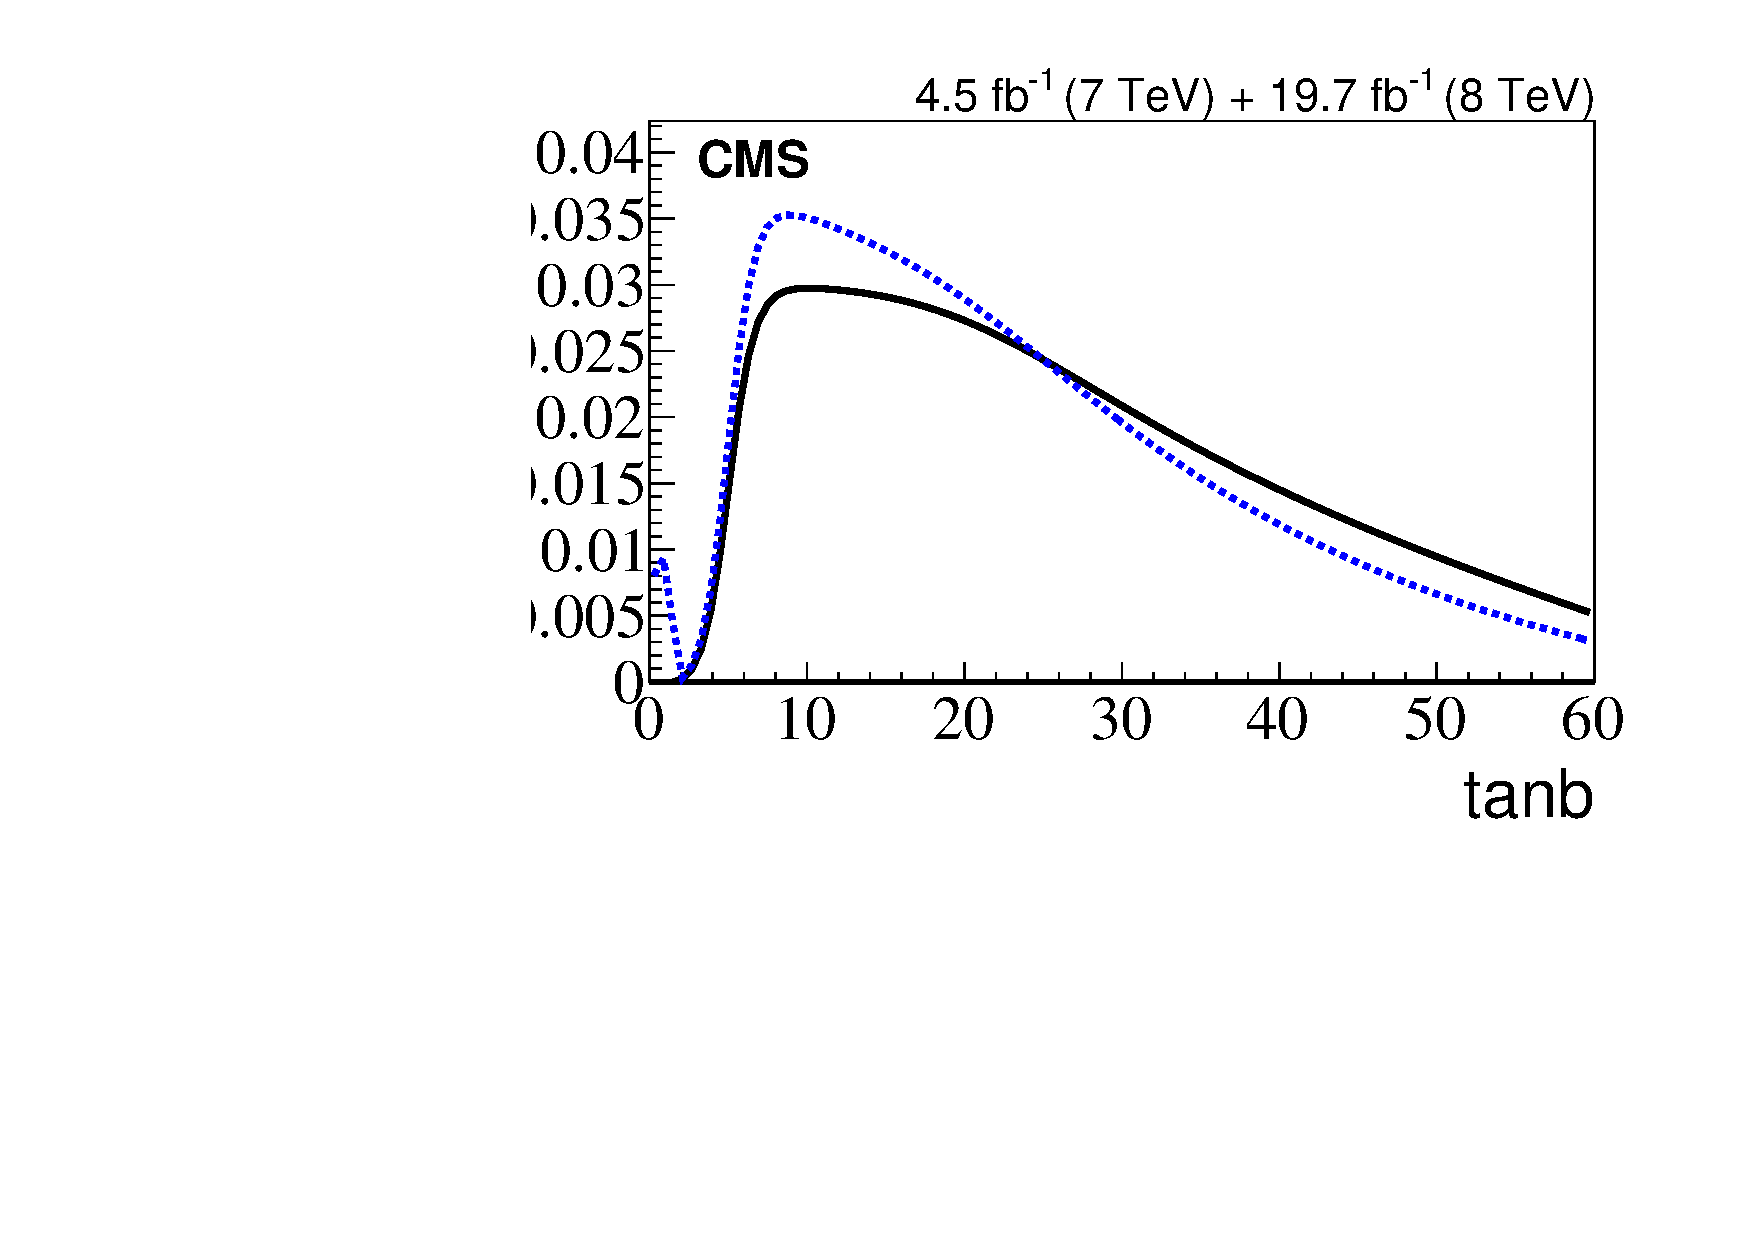
\includegraphics[width=65mm]{figures/pMSSMpaper/Prior/CompareFrequentist/CompareProfileLhdWithPriortanb}
}
\caption{Comparison of the frequentist profile likelihood (dashed blue line) to the non-DCS prior (solid black line) for 6 of the pMSSM parameters. }
\label{fig:PandP1}
\end{figure}


\FloatBarrier

\renewcommand*\thesubfigure{\arabic{subfigure}}
\begin{figure}[htbp]
\centering
\hspace{2mm}
\subfloat[]{
  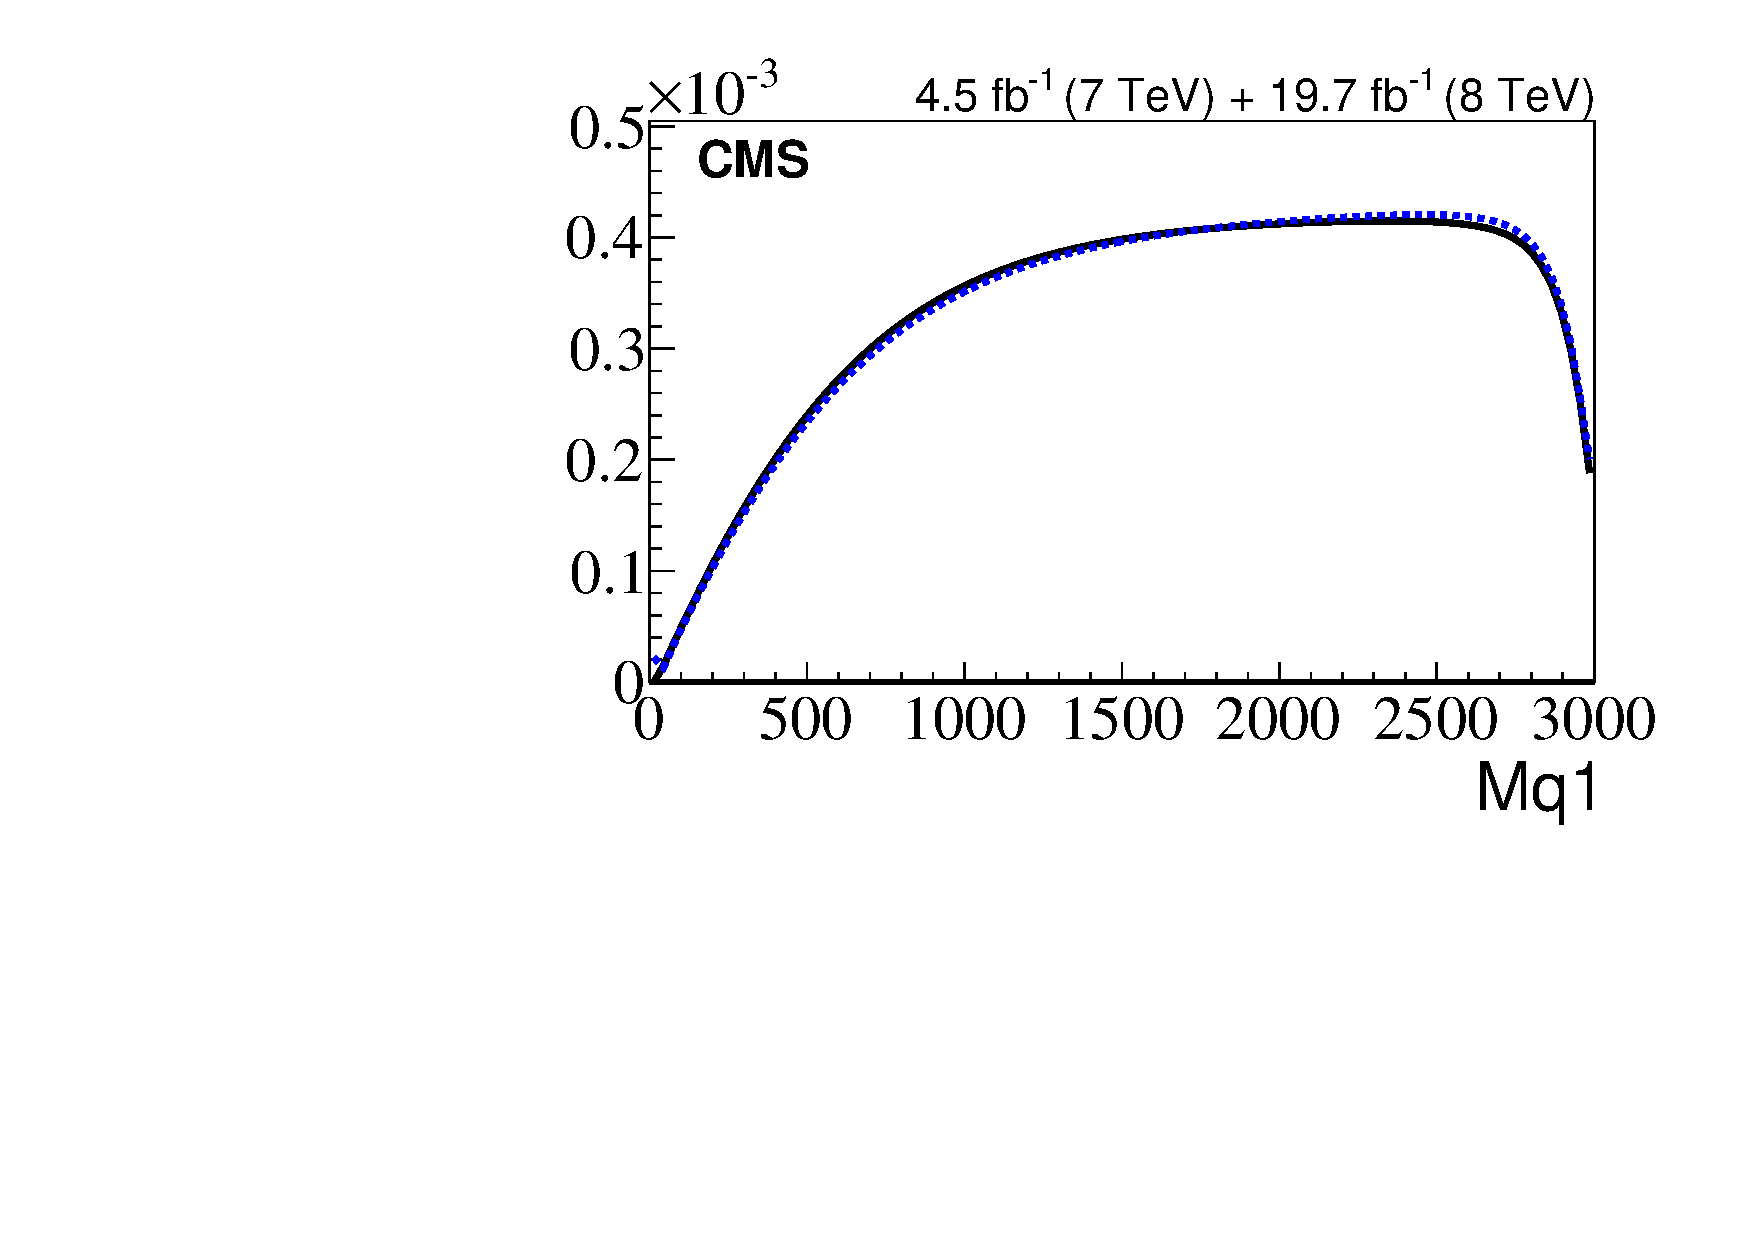
\includegraphics[width=65mm]{figures/pMSSMpaper/Prior/CompareFrequentist/CompareProfileLhdWithPriorMq1}
}
\hspace{2mm}
\subfloat[]{
  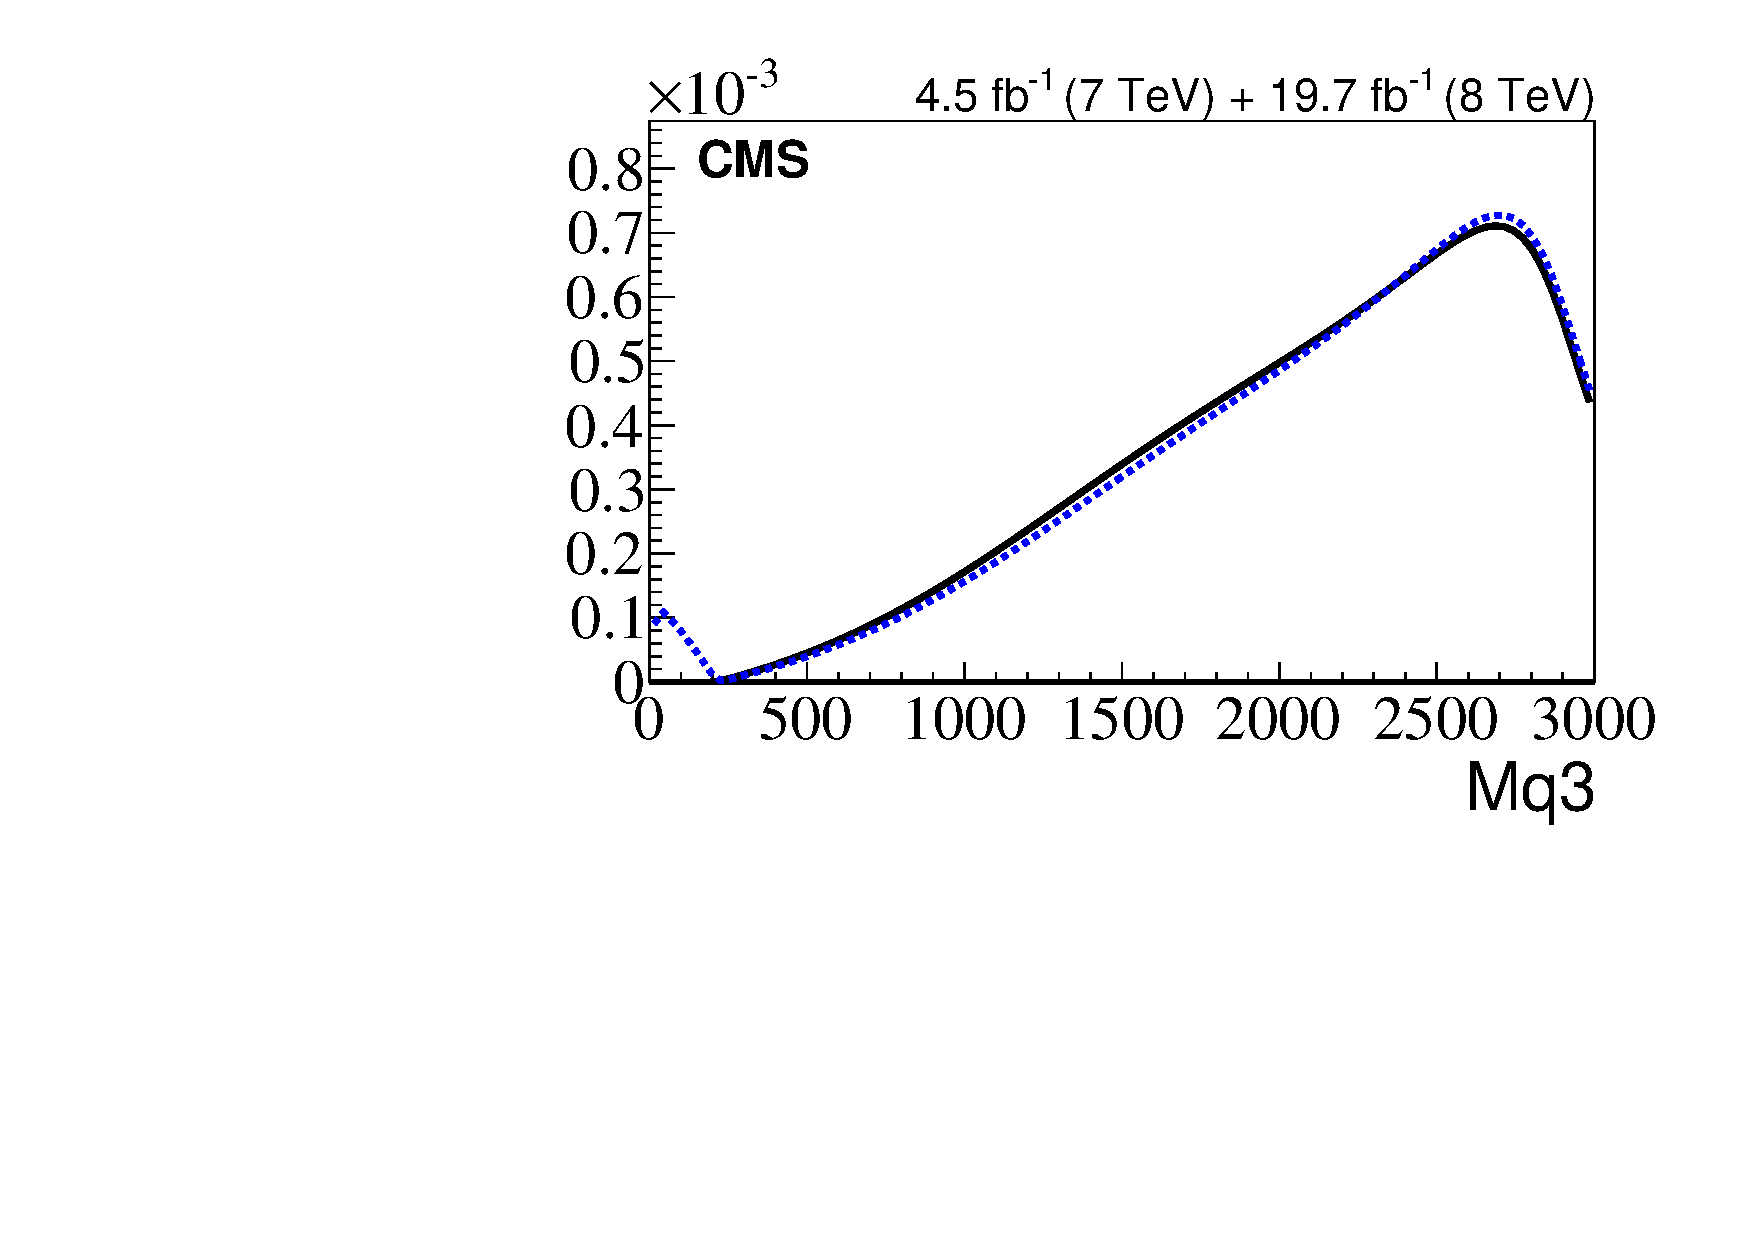
\includegraphics[width=65mm]{figures/pMSSMpaper/Prior/CompareFrequentist/CompareProfileLhdWithPriorMq3}
}
\hspace{2mm}
\subfloat[]{
  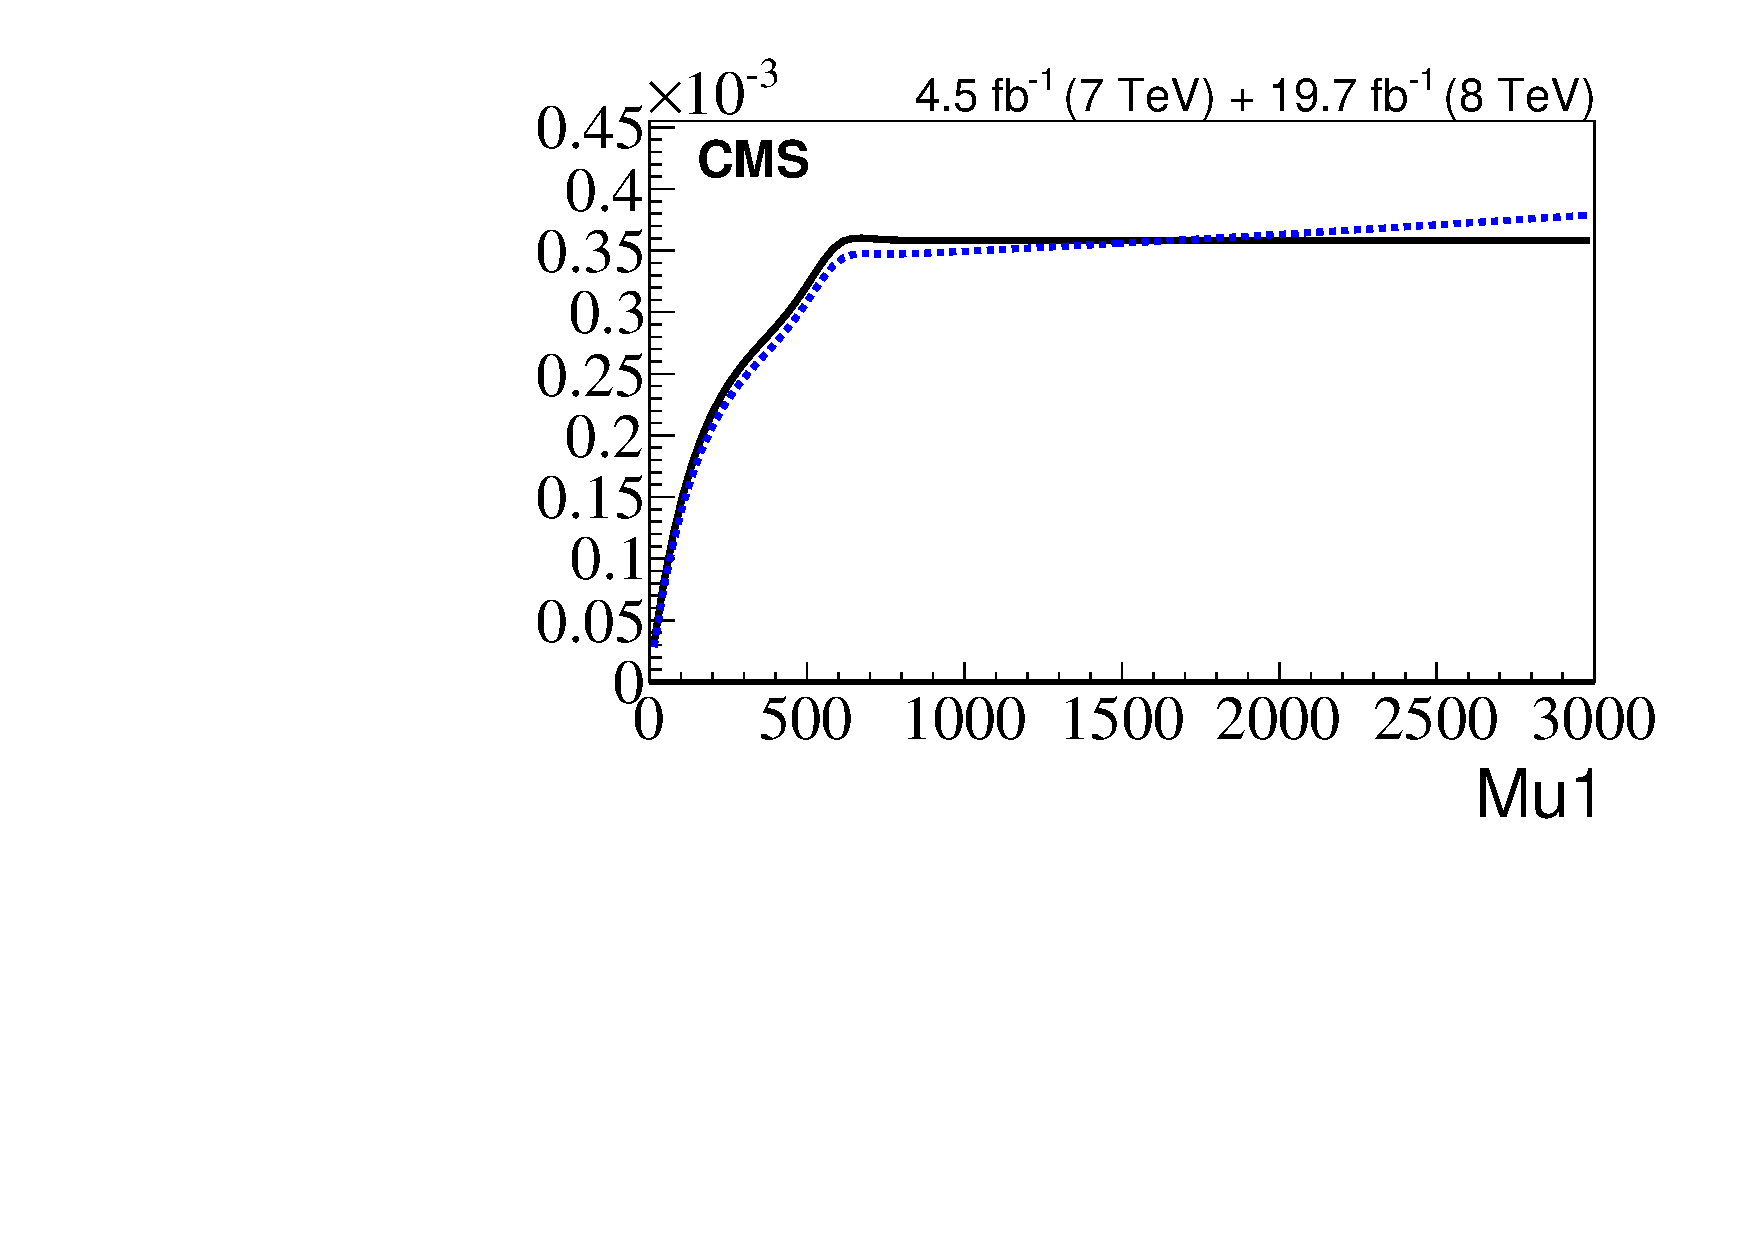
\includegraphics[width=65mm]{figures/pMSSMpaper/Prior/CompareFrequentist/CompareProfileLhdWithPriorMu1}
}
\hspace{2mm}
\subfloat[]{
  \includegraphics[width=65mm]{figures/pMSSMpaper/Prior/CompareFrequentist/CompareProfileLhdWithPriorMu3}
}
\hspace{2mm}
\subfloat[]{
  \includegraphics[width=65mm]{figures/pMSSMpaper/Prior/CompareFrequentist/CompareProfileLhdWithPriorMd1}
}
\hspace{2mm}
\subfloat[]{
  \includegraphics[width=65mm]{figures/pMSSMpaper/Prior/CompareFrequentist/CompareProfileLhdWithPriorMd3}
}
\caption{Comparison of the frequentist profile likelihood (dashed blue line) to the non-DCS prior (solid black line) for an additional 6 of the pMSSM parameters. }
\label{fig:PandP2}
\end{figure}

\FloatBarrier

\renewcommand*\thesubfigure{\arabic{subfigure}}
\begin{figure}[htbp]
\centering
\hspace{2mm}
\subfloat[]{
  \includegraphics[width=65mm]{figures/pMSSMpaper/Prior/CompareFrequentist/CompareProfileLhdWithPriorMl1}
}
\hspace{2mm}
\subfloat[]{
  \includegraphics[width=65mm]{figures/pMSSMpaper/Prior/CompareFrequentist/CompareProfileLhdWithPriorMl3}
}
\hspace{2mm}
\subfloat[]{
  \includegraphics[width=65mm]{figures/pMSSMpaper/Prior/CompareFrequentist/CompareProfileLhdWithPriorMr1}
}
\hspace{2mm}
\subfloat[]{
  \includegraphics[width=65mm]{figures/pMSSMpaper/Prior/CompareFrequentist/CompareProfileLhdWithPriorMr3}
}
\hspace{2mm}
\subfloat[]{
  \includegraphics[width=65mm]{figures/pMSSMpaper/Prior/CompareFrequentist/CompareProfileLhdWithPriorAt}
}
\hspace{2mm}
\subfloat[]{
  \includegraphics[width=65mm]{figures/pMSSMpaper/Prior/CompareFrequentist/CompareProfileLhdWithPriorAb}
}
\caption{Comparison of the frequentist profile likelihood (dashed blue line) to the non-DCS prior (solid black line) for an additional 6 of the pMSSM parameters. }
\label{fig:PandP3}
\end{figure}

\FloatBarrier

\renewcommand*\thesubfigure{\arabic{subfigure}}
\begin{figure}[htbp]
\centering
\hspace{2mm}
\subfloat[]{
  \includegraphics[width=65mm]{figures/pMSSMpaper/Prior/CompareFrequentist/CompareProfileLhdWithPriorAl}
}
\caption{Comparison of the frequentist profile likelihood (dashed blue line) to the non-DCS prior (solid black line) for a pMSSM parameter. }
\label{fig:PandP4}
\end{figure}